% .Id: $Author: kdavis $ on $Date: 2003/06/26 19:29:31 $ ($Revision: 1.2 $)

\documentclass[$Date: 2003/06/26 19:29:31 $]{glabarticle}

\ifpdf
\usepackage[pdftex,
            colorlinks=true,
            linkcolor=blue,
            citecolor=blue,
            urlcolor=blue,
            bookmarks=true,
            bookmarksnumbered=true,
            pdftitle={GAT Java API Specification},
            pdfauthor={Tom Goodale, Kelly Davis},
            pdfsubject={GAT Java API Specification},
            pdfkeywords={Java API GAT GridLab WP1}     
           ]{hyperref}
\usepackage{thumbpdf}
\else
\usepackage{hyperref}
\fi

\usepackage{ifthen}
\usepackage{calc}

\newcommand{\selfreference}[1]{\href{#1}{#1}}

%===============================================================================

\begin{document}

%===============================================================================

\glabdocauthors  {Kelly Davis, Tom Goodale}
\glabdoctitle    {GAT Java API Specification}
\glabwpname      {Grid Application Toolkit}
\glabdocfilename {Gridlab-1-GJAS-0009.JavaAPISpecification}
\glabpartners{PSNC,ZIB,MU,SZTAKI,VU,ISUFI,CARDIFF,GRIDWARE,\\COMPAQ,NTUA}
\glableadpartner{MPG}
\glabconfigid{GridLab-1-GJAS-0009-0.1DRAFT}
\glabdocclas     {Internal}
\glababstract    { 
This document describes the Java binding of the GAT API.
}

\glablastamendment{\getcvsdate~~--~~\getcvstime} 

%===============================================================================

\glabmaketitle

%===============================================================================

\tableofcontents

\newpage

%%%%%%%%%%%%%%%%%%%%%%%%%%%%%%%%%%%%%%%%%%%%%%%%%%%%%%%%%%%%%%%%%%%%%%%%%%%%%%%%
%%%%%%%%%%%%%%%%%%%%%%%%%%%%%%%%%%%%%%%%%%%%%%%%%%%%%%%%%%%%%%%%%%%%%%%%%%%%%%%%
%%%%%%%%%%%%%%%%%%%%%%%%%%%%%%%%%%%%%%%%%%%%%%%%%%%%%%%%%%%%%%%%%%%%%%%%%%%%%%%%

\section{Introduction}

The GAT API provides an abstraction layer which abstracts operations
which may need to be Grid-aware in such a way that an application may
be developed and run independently of the underlying middle-ware
actually deployed.

The GAT consists of a jar --- {\bf the GAT Engine} --- which all GAT enabled
applications have in their classpath, and a set of {\bf adaptors} which
provide the bindings between the operations called in the application and the
underlying providers, e.g. grid services.  The technical reasons for
this are outlined in the GAT Technical Specification~\cite{GridLab-D1.2}.

The APIs can be split into four parts:

\begin{itemize}
\item GAT Application API

      This is the API which provides the ``grid'' operations.

\item GAT Application Utility API

      These are GAT Engine management and interaction operations which
      an application needs to call to interact with the GAT.

\item  GAT Adaptor  API

      This is the mirror of GAT Application API and is the way in
      which adaptors provide those functions.

\item GAT Adaptor Utility API

      These are the additional functions an adaptor needs to interact
      with the GATEngine and possibly with other adaptors and utility
      libraries.

Since the GAT is an adaption layer we cannot enforce security at the
API level, however we will provide functions which allow the
application to specify credential information to the underlying
adaptors which these may then use to authenticate to services and
delegate, as determined by the underlying security model of these
services.

\end{itemize}

%%%%%%%%%%%%%%%%%%%%%%%%%%%%%%%%%%%%%%%%%%%%%%%%%%%%%%%%%%%%%%%%%%%%%%%%%%%%%%%%
%%%%%%%%%%%%%%%%%%%%%%%%%%%%%%%%%%%%%%%%%%%%%%%%%%%%%%%%%%%%%%%%%%%%%%%%%%%%%%%%

\subsection{Purpose of Document}

This document defines the Java binding of the language-independent description of the GAT
API, based upon a set of classes, their attributes, and methods.  It is the second in a sequence 
of language-dependent API documents; the first in the sequence details the C binding of the
language-independent description of the GAT API.

%%%%%%%%%%%%%%%%%%%%%%%%%%%%%%%%%%%%%%%%%%%%%%%%%%%%%%%%%%%%%%%%%%%%%%%%%%%%%%%%
%%%%%%%%%%%%%%%%%%%%%%%%%%%%%%%%%%%%%%%%%%%%%%%%%%%%%%%%%%%%%%%%%%%%%%%%%%%%%%%%

\subsection{Structure of Document}

This document consists of the follwoing sections.  Section \ref{sec:Packages} details the
various packages, Section \ref{sec:API-Olist} lists all the objects, with brief descriptions, 
section \ref{sec:GAT-App-API} details the operation of the GAT Application API, 
\ref{sec:GAT-App-Util-API} details the GAT  Application Utility API, and section 
\ref{sec:GAT-Adp} details the GAT Adaptor API.

%%%%%%%%%%%%%%%%%%%%%%%%%%%%%%%%%%%%%%%%%%%%%%%%%%%%%%%%%%%%%%%%%%%%%%%%%%%%%%%%
%%%%%%%%%%%%%%%%%%%%%%%%%%%%%%%%%%%%%%%%%%%%%%%%%%%%%%%%%%%%%%%%%%%%%%%%%%%%%%%%

\subsection{Status of this Document}

This document is still a draft.  The API functions are still being worked on and the error states 
have not been finalized.  However it should be taken as a good indication of the set of API functions 
which will be available.

%%%%%%%%%%%%%%%%%%%%%%%%%%%%%%%%%%%%%%%%%%%%%%%%%%%%%%%%%%%%%%%%%%%%%%%%%%%%%%%%
%%%%%%%%%%%%%%%%%%%%%%%%%%%%%%%%%%%%%%%%%%%%%%%%%%%%%%%%%%%%%%%%%%%%%%%%%%%%%%%%

\subsection{RFC 2119 and this Document}
The key words ``MUST'', ``MUST NOT'', ``REQUIRED'', ``SHALL'', ``SHALL
NOT'', ``SHOULD'', ``SHOULD NOT'', ``RECOMMENDED'', ``MAY'', and
``OPTIONAL'' in this document are to be interpreted as described in RFC
2119 \cite{RFC2119}.

%%%%%%%%%%%%%%%%%%%%%%%%%%%%%%%%%%%%%%%%%%%%%%%%%%%%%%%%%%%%%%%%%%%%%%%%%%%%%%%%
%%%%%%%%%%%%%%%%%%%%%%%%%%%%%%%%%%%%%%%%%%%%%%%%%%%%%%%%%%%%%%%%%%%%%%%%%%%%%%%%
%%%%%%%%%%%%%%%%%%%%%%%%%%%%%%%%%%%%%%%%%%%%%%%%%%%%%%%%%%%%%%%%%%%%%%%%%%%%%%%%

\newpage

\section{GAT Application API Package List}
\label{sec:Packages}

This section describes the various packages which are part of the GAT Application API. Each package is
identified and a short package description is given indicating the functionality of the various contained
elements. 

\subsection{org.gridlab.gat}

This package contains classes and interfaces which are used throughout the GAT application API. The
most important classes are GATContext and Preferences. An instance of the class GATCOntext is the
primary GAT state object and is used to broker resources on behalf of the user. An instance of the class
Preferences represents user preferences and is used to indicate the user's preferences in selecting
which adaptors are apropos for the user's needs. 

\subsection{org.gridlab.gat.io}

This package contains classes and interfaces which are used to provide input and output employing 
streams and the file system. The most important classes and interfaces are File, LogicalFile, Streamable,
Stream, FileStream, and the corresponding capability provider interfaces. An instance of the class File
is an abstract representation of a physical file and is used to preform operations on an entire file.
An instance of the class LogicalFile is an abstract representation of a set of identical physical files
and is used to facilitate data transfer. The Streamable interface specifies the methods that a class
representing a connection to an external entity must implement. An instance of the class Stream
represents an open connection to another process and is used to send data to other processes.
An instance of the class FileStream represents an open file and is used to read data from and write
data to an open file.The various capability provider interfaces are used by an adaptor writer to 
implement the functionality contained in this package. 

\subsection{org.gridlab.gat.monitoring}

This package contains classes and interfaces which are used to monitor resources. The most important
classes and interfaces in this package are Metric, MetricEvent, MetricListener, and Monitorable. An 
instance of the class Metric represents a measurable quantity within a monitoring system and is used to specify
a measurable quantity. An instance of the class MetricEvent represents the measured value of a
quantity measured by a monitoring system and is used to specify to interested parties that a measurement
of a quantity corresponding to a Metric has taken place. The interface MetricListener is implemented by
classes which wish to be informed of MetricEvents and is used to inform instances of such classes of
MetricEvent's. The interface Monitorable is implemented by classes which wish to be monitored for
MetricEvents and is used to inform interested parties of such events.

\subsection{org.gridlab.gat.net}

This package contains the classes and interfaces which are used for networking. Currently the only class
in this package is the Location class. An instance of the class Location represents the location of an
abstract or physical resource and is used to specify such.

\subsection{org.gridlab.gat.resources}

This package contains the classes and interfaces which are used for using resources, be they hardware
or software resources. The most important classes and interfaces in this package are ResourceBroker
and Reservation. An instance of the class ResourceBroker represents a broker for resources and is used 
to reserve and find resources. An instance of the class Reservation represents a reservation for a
resource and is used to manipulate this reservation.

\subsection{org.gridlab.gat.resources.hardware}

This package contains the classes and interfaces which are required to use and manipulate hardware
resources. The most important classes and interfaces in this package are HardwareResourceDescription
and HardwareResource. An instance of the class HardwareResourceDescription represents a description
of a hardware resource and is used to describe such. An instance of the class HardwareResource represents
a hardware resource and is used to manipulate such..

\subsection{org.gridlab.gat.resources.software}

THis package contains the classes and interfaces which are required to use and manipulate software
resources. The most important classes and interfaces in this package are SoftwareResourceDescription,
SimpleJob, and CheckpointableSimpleJob, An instance of the class SoftwareResourceDescription represents
a description of a software resource and is used to describe such. An instance of the class SimpleJob
represents a job which requires the start of a single executable which can be monitored and is used
to manipulate such. An instance of the class CheckpointableSimpleJob represents a SimpleJob
which is checkpointable and is used to manipulate such a job.

\subsection{org.gridlab.gat.security}

This package contains classes and interfaces which are required to secure software and hardware resources.
Currently the only class in this package is SecurityContext. An instance of the class SecurityContext contains
security information which can be used to secure software and hardware resources. 

\subsection{org.gridlab.gat.util}

This package contains classes and interfaces which are of general use for the GAT application API. The
most important classes and interfaces in this package are Collection, TimePeriod, and Buffer. An instance
of the class Collection represents a collection, a group of objects which are known as elements, and is used
to manipulate such. An instance of the class TimePeriod represents a time period. An instance of the
class Buffer is a container for data.

%%%%%%%%%%%%%%%%%%%%%%%%%%%%%%%%%%%%%%%%%%%%%%%%%%%%%%%%%%%%%%%%%%%%%%%%%%%%%%%%
%%%%%%%%%%%%%%%%%%%%%%%%%%%%%%%%%%%%%%%%%%%%%%%%%%%%%%%%%%%%%%%%%%%%%%%%%%%%%%%%
%%%%%%%%%%%%%%%%%%%%%%%%%%%%%%%%%%%%%%%%%%%%%%%%%%%%%%%%%%%%%%%%%%%%%%%%%%%%%%%%

\newpage

\section{API Object List}
\label{sec:API-Olist}

%%%%%%%%%%%%%%%%%%%%%%%%%%%%%%%%%%%%%%%%%%%%%%%%%%%%%%%%%%%%%%%%%%%%%%%%%%%%%%%%
%%%%%%%%%%%%%%%%%%%%%%%%%%%%%%%%%%%%%%%%%%%%%%%%%%%%%%%%%%%%%%%%%%%%%%%%%%%%%%%%

\subsection{GAT Application API Classes and Interfaces}

%%%%%%%%%%%%%%%%%%%%%%%%%%%%%%%%%%%%%%%%%%%%%%%%%%%%%%%%%%%%%%%%%%%%%%%%%%%%%%%%
% KJD: Done!
\subsubsection{org.gridlab.gat.monitoring.Monitorable}

Interface which is to be implemented by any classes which are capable of being monitored.

%%%%%%%%%%%%%%%%%%%%%%%%%%%%%%%%%%%%%%%%%%%%%%%%%%%%%%%%%%%%%%%%%%%%%%%%%%%%%%%%
% KJD: Done!
\subsubsection{org.gridlab.gat.io.File}

Class which is an abstract representation of a physical file.

%%%%%%%%%%%%%%%%%%%%%%%%%%%%%%%%%%%%%%%%%%%%%%%%%%%%%%%%%%%%%%%%%%%%%%%%%%%%%%%%
% KJD: Done!
\subsubsection{org.gridlab.gat.io.FileCpi}

Capability provider interface to the File class.

%%%%%%%%%%%%%%%%%%%%%%%%%%%%%%%%%%%%%%%%%%%%%%%%%%%%%%%%%%%%%%%%%%%%%%%%%%%%%%%%
% KJD: Done!
\subsubsection{org.gridlab.gat.io.LogicalFile}

Class which is an abstract representation of a set of identical physical files.

%%%%%%%%%%%%%%%%%%%%%%%%%%%%%%%%%%%%%%%%%%%%%%%%%%%%%%%%%%%%%%%%%%%%%%%%%%%%%%%%
% KJD: Done!
\subsubsection{org.gridlab.gat.io.LogicalFileCpi}

Capability provider interface to the LogicalFile class.

%%%%%%%%%%%%%%%%%%%%%%%%%%%%%%%%%%%%%%%%%%%%%%%%%%%%%%%%%%%%%%%%%%%%%%%%%%%%%%%%
% KJD: Done!
\subsubsection{org.gridlab.gat.resources.software.SimpleJob}

An instance of this class represents a monitorable simple job, a job
which requires the start of a single executable, which is monitorable.

%%%%%%%%%%%%%%%%%%%%%%%%%%%%%%%%%%%%%%%%%%%%%%%%%%%%%%%%%%%%%%%%%%%%%%%%%%%%%%%%
% KJD: Done!
\subsubsection{org.gridlab.gat.resources.software.SimpleJobCpi}

Capability provider interface to the SimpleJob class.

%%%%%%%%%%%%%%%%%%%%%%%%%%%%%%%%%%%%%%%%%%%%%%%%%%%%%%%%%%%%%%%%%%%%%%%%%%%%%%%%
% KJD: Done!
\subsubsection{org.gridlab.gat.resources.software.CheckpointableSimpleJob}

An instance of this class represents a checkpointable, monitorable
simple job, a job which requires the start of a single executable and
is checkpointable and monitorable.

%%%%%%%%%%%%%%%%%%%%%%%%%%%%%%%%%%%%%%%%%%%%%%%%%%%%%%%%%%%%%%%%%%%%%%%%%%%%%%%%
% KJD: Done!
\subsubsection{org.gridlab.gat.resources.software.CheckpointableSimpleJobCpi}

Capability provider interface to the CheckpointableSimpleJob class.

%%%%%%%%%%%%%%%%%%%%%%%%%%%%%%%%%%%%%%%%%%%%%%%%%%%%%%%%%%%%%%%%%%%%%%%%%%%%%%%%
% KJD: Done!
\subsubsection{org.gridlab.gat.resources.software.SoftwareResourceDescription}

An instance of this class is a description of a software resource, a
logical thing, which a may be required by a hardware or software
component.

%%%%%%%%%%%%%%%%%%%%%%%%%%%%%%%%%%%%%%%%%%%%%%%%%%%%%%%%%%%%%%%%%%%%%%%%%%%%%%%%
% KJD: Done!
\subsubsection{org.gridlab.gat.resources.hardware.HardwareResourceDescription}

An instance of this class is a description of a hardware resource, a
physical thing, which a may be required by a hardware or software
component.

%%%%%%%%%%%%%%%%%%%%%%%%%%%%%%%%%%%%%%%%%%%%%%%%%%%%%%%%%%%%%%%%%%%%%%%%%%%%%%%%
% KJD: Done!
\subsubsection{org.gridlab.gat.resources.hardware.HardwareResource}

An instance of this class is an abstract representation of a physical
hardware resource which is monitorable.

%%%%%%%%%%%%%%%%%%%%%%%%%%%%%%%%%%%%%%%%%%%%%%%%%%%%%%%%%%%%%%%%%%%%%%%%%%%%%%%%
% KJD: Done!
\subsubsection{org.gridlab.gat.io.Streamable}

A class implementing the Streamable interface represents a connection to an external entity 
such as a file or another process. 

%%%%%%%%%%%%%%%%%%%%%%%%%%%%%%%%%%%%%%%%%%%%%%%%%%%%%%%%%%%%%%%%%%%%%%%%%%%%%%%%
% KJD: Done
\subsubsection{org.gridlab.gat.io.Stream}

A Stream class represents an open connection to another process. This class implements the Streamable interface.

%%%%%%%%%%%%%%%%%%%%%%%%%%%%%%%%%%%%%%%%%%%%%%%%%%%%%%%%%%%%%%%%%%%%%%%%%%%%%%%%
% KJD: Done!
\subsubsection{org.gridlab.gat.io.StreamCpi}

Capability provider interface to the Stream class.

%%%%%%%%%%%%%%%%%%%%%%%%%%%%%%%%%%%%%%%%%%%%%%%%%%%%%%%%%%%%%%%%%%%%%%%%%%%%%%%%
% KJD: Done!
\subsubsection{org.gridlab.gat.io.FileStream}

A FileStream class represents an open file.  This class implements the Streamable interface.

%%%%%%%%%%%%%%%%%%%%%%%%%%%%%%%%%%%%%%%%%%%%%%%%%%%%%%%%%%%%%%%%%%%%%%%%%%%%%%%%
% KJD: Done!
\subsubsection{org.gridlab.gat.io.FileStreamCpi}

Capability provider interface to the FileStream class.

%%%%%%%%%%%%%%%%%%%%%%%%%%%%%%%%%%%%%%%%%%%%%%%%%%%%%%%%%%%%%%%%%%%%%%%%%%%%%%%%
% KJD: Done!
\subsubsection{org.gridlab.gat.resources.ResourceBroker}

An instance of this class is used to reserve resources

%%%%%%%%%%%%%%%%%%%%%%%%%%%%%%%%%%%%%%%%%%%%%%%%%%%%%%%%%%%%%%%%%%%%%%%%%%%%%%%%
% KJD: Done!
\subsubsection{org.gridlab.gat.resources.ResourceBrokerCpi}

Capability provider interface to the ResourceBroker class.

%%%%%%%%%%%%%%%%%%%%%%%%%%%%%%%%%%%%%%%%%%%%%%%%%%%%%%%%%%%%%%%%%%%%%%%%%%%%%%%%
% KJD: Done!
\subsubsection{org.gridlab.gat.resources.Reservation}

An instance of this class represents a reservation for resources

%%%%%%%%%%%%%%%%%%%%%%%%%%%%%%%%%%%%%%%%%%%%%%%%%%%%%%%%%%%%%%%%%%%%%%%%%%%%%%%%
% KJD: Done!
\subsubsection{org.gridlab.gat.util.Collection}

An instance of this class represents a collection, a group of objects which are known as elements.

%%%%%%%%%%%%%%%%%%%%%%%%%%%%%%%%%%%%%%%%%%%%%%%%%%%%%%%%%%%%%%%%%%%%%%%%%%%%%%%%
% KJD: Done!
\subsubsection{org.gridlab.gat.util.CollectionCpi}

Capability provider interface to the Collection class.

%%%%%%%%%%%%%%%%%%%%%%%%%%%%%%%%%%%%%%%%%%%%%%%%%%%%%%%%%%%%%%%%%%%%%%%%%%%%%%%%
% KJD: Done!
\subsubsection{org.gridlab.gat.monitoring.Metric}

An instance of this class represents a measurable quantity within a monitoring system.

%%%%%%%%%%%%%%%%%%%%%%%%%%%%%%%%%%%%%%%%%%%%%%%%%%%%%%%%%%%%%%%%%%%%%%%%%%%%%%%%
% KJD: Done!
\subsubsection{org.gridlab.gat.monitoring.MetricEvent}

An instance of this class represents an metric event.

%%%%%%%%%%%%%%%%%%%%%%%%%%%%%%%%%%%%%%%%%%%%%%%%%%%%%%%%%%%%%%%%%%%%%%%%%%%%%%%%
% KJD: Done!
\subsubsection{org.gridlab.gat.monitoring.MetricListener}

An instance of a class implementing this interface can receive MetricEvents.

%%%%%%%%%%%%%%%%%%%%%%%%%%%%%%%%%%%%%%%%%%%%%%%%%%%%%%%%%%%%%%%%%%%%%%%%%%%%%%%%
% KJD: Done!
\subsubsection{org.gridlab.gat.Preferences}

An instance of this class represents user preferences. 

%%%%%%%%%%%%%%%%%%%%%%%%%%%%%%%%%%%%%%%%%%%%%%%%%%%%%%%%%%%%%%%%%%%%%%%%%%%%%%%%
%%%%%%%%%%%%%%%%%%%%%%%%%%%%%%%%%%%%%%%%%%%%%%%%%%%%%%%%%%%%%%%%%%%%%%%%%%%%%%%%

\subsection{GAT Application Utility API Objects}

Not only must the API provide a set of calls for abstract grid operations, but an implementation must provide 
calls to initialise the library and do management tasks.

%%%%%%%%%%%%%%%%%%%%%%%%%%%%%%%%%%%%%%%%%%%%%%%%%%%%%%%%%%%%%%%%%%%%%%%%%%%%%%%%
% KJD: Done!
\subsubsection{org.gridlab.gat.GATContext}

An instance of this class is the primary GAT state object.

%%%%%%%%%%%%%%%%%%%%%%%%%%%%%%%%%%%%%%%%%%%%%%%%%%%%%%%%%%%%%%%%%%%%%%%%%%%%%%%%
% KJD: Done!
\subsubsection{org.gridlab.gat.security.SecurityContext}

An instance of this class contains security information which can be associated with a GAT context.

%%%%%%%%%%%%%%%%%%%%%%%%%%%%%%%%%%%%%%%%%%%%%%%%%%%%%%%%%%%%%%%%%%%%%%%%%%%%%%%%
% KJD: Done!
\subsubsection{org.gridlab.gat.net.Location} 

An instance of this class represents the location of an abstract or physical resource.

%%%%%%%%%%%%%%%%%%%%%%%%%%%%%%%%%%%%%%%%%%%%%%%%%%%%%%%%%%%%%%%%%%%%%%%%%%%%%%%%
% KJD: Done!
\subsubsection{org.gridlab.gat.util.TimePeriod}

An instance of this class represents a time period

%%%%%%%%%%%%%%%%%%%%%%%%%%%%%%%%%%%%%%%%%%%%%%%%%%%%%%%%%%%%%%%%%%%%%%%%%%%%%%%%
% KJD: Done!
\subsubsection{org.gridlab.gat.util.Buffer}

A container for data.

%%%%%%%%%%%%%%%%%%%%%%%%%%%%%%%%%%%%%%%%%%%%%%%%%%%%%%%%%%%%%%%%%%%%%%%%%%%%%%%%
%%%%%%%%%%%%%%%%%%%%%%%%%%%%%%%%%%%%%%%%%%%%%%%%%%%%%%%%%%%%%%%%%%%%%%%%%%%%%%%%

\subsection{GAT Adaptor API}

This section covers the means by which adaptors register and provide functionality.

%%%%%%%%%%%%%%%%%%%%%%%%%%%%%%%%%%%%%%%%%%%%%%%%%%%%%%%%%%%%%%%%%%%%%%%%%%%%%%%%
%%%%%%%%%%%%%%%%%%%%%%%%%%%%%%%%%%%%%%%%%%%%%%%%%%%%%%%%%%%%%%%%%%%%%%%%%%%%%%%%

\subsection{GAT Adaptor Utility API}

The Adaptor Utility API is not covered in this document.

%%%%%%%%%%%%%%%%%%%%%%%%%%%%%%%%%%%%%%%%%%%%%%%%%%%%%%%%%%%%%%%%%%%%%%%%%%%%%%%%
%%%%%%%%%%%%%%%%%%%%%%%%%%%%%%%%%%%%%%%%%%%%%%%%%%%%%%%%%%%%%%%%%%%%%%%%%%%%%%%%
%%%%%%%%%%%%%%%%%%%%%%%%%%%%%%%%%%%%%%%%%%%%%%%%%%%%%%%%%%%%%%%%%%%%%%%%%%%%%%%%

\newpage

\section{GAT Application API Object Descriptions}
\label{sec:GAT-App-API}

This section defines the publicly accessible methods and attributes
associated with each object.  Note that private data is an
implementation and language-specific detail and is thus not part of
the API.  The words ``Constructor'' and ``Destructor'' have been used
to denote the methods used for creation and destruction of each
object, however the actual names of these methods, and whether they
must be explicitly called by the application, are language dependent.

Also some objects may ``inherit'' methods from other objects, but this too
is language dependent --- e.g. in Java this may be done via interfaces.

%%%%%%%%%%%%%%%%%%%%%%%%%%%%%%%%%%%%%%%%%%%%%%%%%%%%%%%%%%%%%%%%%%%%%%%%%%%%%%%%
%%%%%%%%%%%%%%%%%%%%%%%%%%%%%%%%%%%%%%%%%%%%%%%%%%%%%%%%%%%%%%%%%%%%%%%%%%%%%%%%

\newpage

\subsection{public interface Monitorable}

%%%%%%%%%%%%%%%%%%%%%%%%%%%%%%%%%%%%%%%%%%%%%%%%%%%%%%%%%%%%%%%%%%%%%%%%%%%%%%%%

\subsubsection{Description}

Interface which is to be implemented by any classes which are capable of being monitored.

%%%%%%%%%%%%%%%%%%%%%%%%%%%%%%%%%%%%%%%%%%%%%%%%%%%%%%%%%%%%%%%%%%%%%%%%%%%%%%%%

\subsubsection{Methods}

 \paragraph{public void AddMetricListener}
 
 This method adds the passed instance of a MetricListener to the java.util.List
 of MetricListeners which are notified of MetricEvents by an
 instance of this class. The passed MetricListener is only notified of
 MetricEvents which correspond to Metric instance passed to this
 method. \\
 
 \textit{Parameters}:
 \begin{itemize}
 \item[] MetricListener --- The MetricListener to notify of MetricEvents
 \item[] Metric --- The Metric corresponding to the MetricEvents for which the passed MetricListener will be 
 notified
 \end{itemize}
 
 \textit{Throws}:
 \begin{itemize}
 \item[] java.rmi.RemoteException --- Thrown upon problems accessing the remote instance 
 \end{itemize}
 
 \paragraph{public void RemoveMetricListener}
 
 Removes the passed MetricListener from the java.util.List of MetricListeners
 which are notified of MetricEvents corresponding to the passed
 Metric instance. \\
 
 \textit{Parameters}:
 \begin{itemize}
 \item[] MetricListener --- The MetricListener to notify of MetricEvents
 \item[] metric --- The Metric corresponding to the MetricEvents for which the passed MetricListener has been
 notified
 \end{itemize}
 
 \textit{Throws}:
 \begin{itemize}
 \item[] java.rmi.RemoteException --- Thrown upon problems accessing the remote instance 
 \end{itemize}
  
 \paragraph{public java.util.List GetMetrics}
 
 This method returns a java.util.List of Metric instances. Each Metric instance
 in this java.util.List is a Metric which can be monitored on this instance. \\
 
  \textit{Returns}:
 \begin{itemize}
 \item[] An java.util.List of Metric instances. Each Metric instance in this java.util.List is a Metric which can be
 monitored on this instance.
 \end{itemize} 
 
 \textit{Throws}:
 \begin{itemize}
 \item[] java.rmi.RemoteException --- Thrown upon problems accessing the remote instance 
 \end{itemize}
 
%%%%%%%%%%%%%%%%%%%%%%%%%%%%%%%%%%%%%%%%%%%%%%%%%%%%%%%%%%%%%%%%%%%%%%%%%%%%%%%%

\subsubsection{Attributes}

Monitorable has no publicly available member variables. 

%%%%%%%%%%%%%%%%%%%%%%%%%%%%%%%%%%%%%%%%%%%%%%%%%%%%%%%%%%%%%%%%%%%%%%%%%%%%%%%%
%%%%%%%%%%%%%%%%%%%%%%%%%%%%%%%%%%%%%%%%%%%%%%%%%%%%%%%%%%%%%%%%%%%%%%%%%%%%%%%%

\newpage

\subsection{public class File implements Monitorable}

%%%%%%%%%%%%%%%%%%%%%%%%%%%%%%%%%%%%%%%%%%%%%%%%%%%%%%%%%%%%%%%%%%%%%%%%%%%%%%%%

\subsubsection{Description}

An abstract representation of a physical file.

An instance of this class presents an abstract, system-independent
view of a physical file. User interfaces and operating systems use
system-dependent pathname strings to identify physical files. GAT,
however, uses an operating system independent pathname string to
identify a physical file. A physical file in GAT is identified by a
URI.

An instance of this File class allows for various high-level
operations to be preformed on a physical file. For example, one can,
with a single API call, copy a physical file from one location to a
second location, move a physical file from one location to a second
location, delete a physical file, and preform various other operations
on a physical file. The utility of this high-level view of a physical
file is multi-fold. The client of an instance of this class does not
have to concern themselves with the details of reading every single
byte of a physical file when all they wish to do is copy the physical
file to a new location. Similarly, a client does not have to deal with
all the various error states that can occur when moving a physical
file ( Have all the various bytes been read correctly? Have all the
various bytes been saved correctly? Did the deletion of the original
file proceed correctly? ); the client simply has to call a single API
call and the physical file is moved.

%%%%%%%%%%%%%%%%%%%%%%%%%%%%%%%%%%%%%%%%%%%%%%%%%%%%%%%%%%%%%%%%%%%%%%%%%%%%%%%%

\subsubsection{Methods}

\paragraph{Constructor}

Constructs a File instance which corresponds to the physical file
identified by the passed Location and whose access rights are
determined by the passed GATContext. \\

\textit{Parameters}:
\begin{itemize}
\item[] Location --- A Location which represents the URI corresponding to the physical file.
\item[] GATContext --- A GATContext which is used to determine the access rights for this File.
\end{itemize}

 \textit{Throws}:
 \begin{itemize}
 \item[] java.lang.Exception --- Thrown upon creation problems 
 \end{itemize}

\paragraph{Constructor}

Constructs a File instance which corresponds to the physical file
identified by the passed Location and whose access rights are
determined by the passed GATContext. \\

\textit{Parameters}:
\begin{itemize}
\item[] Location --- A Location which represents the URI corresponding to the physical file.
\item[] GATContext --- A GATContext which is used to determine the access rights for this File.
\item[] Preferences --- A Preferences which is used to determine the user's preferences for this File.
\end{itemize}

\textit{Throws}:
\begin{itemize}
\item[] java.lang.Exception --- Thrown upon creation problems 
\end{itemize}

\paragraph{public boolean Equals}

Tests this File for equality with the passed Object.

 If the given object is not a File, then this method immediately
 returns false.
 
 If the given object is a File, then it is deemed equal to this
 instance if a Location object constructed from this File's location
 and a Location object constructed from the passed File's Location are
 equal as determined by the Equals method of Location. \\

 \textit{Parameters}:
 \begin{itemize}
 \item[] Object --- The Object to test for equality 
 \end{itemize}
 
 \textit{Returns}:
\begin{itemize}
\item[] A boolean indicating equality
\end{itemize}

\paragraph{public void getLocation}

 This method returns the Location of this File. \\

 \textit{Returns}:
 \begin{itemize}
 \item[] The Location of this file
 \end{itemize}
 
 \textit{Throws}:
 \begin{itemize}
 \item[] java.rmi.RemoteException --- Thrown upon problems accessing the remote instance 
 \end{itemize}
 
\paragraph{public void Copy}

This method copies the physical file represented by this File instance
to a physical file identified by the passed Location. \\

 \textit{Parameters}:
 \begin{itemize}
 \item[] Location --- The Location to which to copy the physical file corresponding to this File instance
 \end{itemize}
 
 \textit{Throws}:
 \begin{itemize}
 \item[] java.rmi.RemoteException --- Thrown upon problems accessing the remote instance 
 \end{itemize}
 
\textit{Throws}:
\begin{itemize}
\item[] java.io.IOException --- Upon non-remote IO problem 
\end{itemize}

\paragraph{public void Move}

This method moves the physical file represented by this File instance
to a physical file identified by the passed Location. \\

 \textit{Parameters}:
 \begin{itemize}
 \item[] Location --- The Location to which to move the physical file corresponding to this File instance
 \end{itemize}
 
 \textit{Throws}:
 \begin{itemize}
 \item[] java.rmi.RemoteException --- Thrown upon problems accessing the remote instance 
 \end{itemize}
 
\textit{Throws}:
\begin{itemize}
\item[] java.io.IOException --- Upon non-remote IO problem 
\end{itemize}
 
\paragraph{public static void Move}

This class method moves the physical file represented by the first specified Location to the second specified 
Location. \\

 \textit{Parameters}:
 \begin{itemize}
 \item[] Source --- The source Location from which to move the physical file
 \item[] Destination --- The destination Location to which to move the physical file at Source
 \end{itemize}
 
 \textit{Throws}:
 \begin{itemize}
 \item[] java.rmi.RemoteException --- Thrown upon problems accessing the remote instance 
 \end{itemize}
 
\textit{Throws}:
\begin{itemize}
\item[] java.io.IOException --- Upon non-remote IO problem 
\end{itemize}
 
\paragraph{public void Delete}

This method deletes the physical file represented by this File instance.

 \textit{Throws}:
 \begin{itemize}
 \item[] java.rmi.RemoteException --- Thrown upon problems accessing the remote instance 
 \end{itemize}
 
\paragraph{public boolean IsReadable}

Returns a boolean indicating if the physical file corresponding to
this instance is readable.\\

\textit{Returns}:
\begin{itemize}
\item[] A boolean indicating readability
\end{itemize}

 \textit{Throws}:
 \begin{itemize}
 \item[] java.rmi.RemoteException --- Thrown upon problems accessing the remote instance 
 \end{itemize}
 
\paragraph{public boolean IsWritable}

Returns a boolean indicating if the physical file corresponding to
this instance is writable.\\

\textit{Returns}:
\begin{itemize}
\item[] A boolean indicating writability
\end{itemize}

 \textit{Throws}:
 \begin{itemize}
 \item[] java.rmi.RemoteException --- Thrown upon problems accessing the remote instance 
 \end{itemize}
 
\paragraph{public long GetLength}

Returns a long indicating the length in bytes of the physical file
corresponding to this instance.\\

\textit{Returns}:
\begin{itemize}
\item[] A long indicating the length in bytes of the physical file corresponding to this instance. 
\end{itemize}

 \textit{Throws}:
 \begin{itemize}
 \item[] java.rmi.RemoteException --- Thrown upon problems accessing the remote instance 
 \end{itemize}
 
\paragraph{public long LastModified}

Returns the number of milliseconds after January 1, 1970, 00:00:00 GMT
at which this file was last modified.\\

\textit{Returns}:
\begin{itemize}
\item[] A long indicating the number of milliseconds after January 1, 1970, 00:00:00 GMT at which this file 
was last modified.
\end{itemize}

 \textit{Throws}:
 \begin{itemize}
 \item[] java.rmi.RemoteException --- Thrown upon problems accessing the remote instance 
 \end{itemize}
 
%%%%%%%%%%%%%%%%%%%%%%%%%%%%%%%%%%%%%%%%%%%%%%%%%%%%%%%%%%%%%%%%%%%%%%%%%%%%%%%%

\subsubsection{Attributes}

File has no publicly available member variables. 

%%%%%%%%%%%%%%%%%%%%%%%%%%%%%%%%%%%%%%%%%%%%%%%%%%%%%%%%%%%%%%%%%%%%%%%%%%%%%%%%
%%%%%%%%%%%%%%%%%%%%%%%%%%%%%%%%%%%%%%%%%%%%%%%%%%%%%%%%%%%%%%%%%%%%%%%%%%%%%%%%

\newpage

\subsection{public abstract class FileCpi implements Monitorable}

%%%%%%%%%%%%%%%%%%%%%%%%%%%%%%%%%%%%%%%%%%%%%%%%%%%%%%%%%%%%%%%%%%%%%%%%%%%%%%%%

\subsubsection{Description}

Capability provider interface to the File class.

Capability provider wishing to provide the functionality of the File class must extend this class and
implement all of the abstract methods in this class. Each abstract method in this class mirrors the
corresponding method in this File class and will be used to implement the corresponding method in
the File class at runtime. 

%%%%%%%%%%%%%%%%%%%%%%%%%%%%%%%%%%%%%%%%%%%%%%%%%%%%%%%%%%%%%%%%%%%%%%%%%%%%%%%%

\subsubsection{Methods}

\paragraph{Constructor}

Constructs a FileCpi instance which corresponds to the physical file
identified by the passed Location and whose access rights are
determined by the passed GATContext. \\

\textit{Parameters}:
\begin{itemize}
\item[] Location --- A Location which represents the URI corresponding to the physical file.
\item[] GATContext --- A GATContext which is used to determine the access rights for this FileCpi.
\end{itemize}

\paragraph{public abstract boolean Equals}

Tests this File for equality with the passed Object.

 If the given object is not a File, then this method immediately
 returns false.
 
 If the given object is a File, then it is deemed equal to this
 instance if a Location object constructed from this File's location
 and a Location object constructed from the passed File's Location are
 equal as determined by the Equals method of Location. \\

 \textit{Parameters}:
 \begin{itemize}
 \item[] Object --- The Object to test for equality 
 \end{itemize}
 
 \textit{Returns}:
\begin{itemize}
\item[] A boolean indicating equality
\end{itemize}

\paragraph{public void getLocation}

 This method returns the Location of this File. \\

 \textit{Returns}:
 \begin{itemize}
 \item[] The Location of this file
 \end{itemize}
 
 \textit{Throws}:
 \begin{itemize}
 \item[] java.rmi.RemoteException --- Thrown upon problems accessing the remote instance 
 \end{itemize}
 
\paragraph{public abstract void Copy}

This method copies the physical file represented by this FileCpi instance
to a physical file identified by the passed Location. \\

 \textit{Parameters}:
 \begin{itemize}
 \item[] Location --- The Location to which to copy the physical file corresponding to this FileCpi instance
 \end{itemize}
 
 \textit{Throws}:
 \begin{itemize}
 \item[] java.rmi.RemoteException --- Thrown upon problems accessing the remote instance 
 \end{itemize}
 
\textit{Throws}:
\begin{itemize}
\item[] java.io.IOException --- Upon non-remote IO problem 
\end{itemize}

\paragraph{public abstract void Move}

This method moves the physical file represented by this FileCpi instance
to a physical file identified by the passed Location. \\

 \textit{Parameters}:
 \begin{itemize}
 \item[] Location --- The Location to which to move the physical file corresponding to this FileCpi instance
 \end{itemize}
 
 \textit{Throws}:
 \begin{itemize}
 \item[] java.rmi.RemoteException --- Thrown upon problems accessing the remote instance 
 \end{itemize}
 
\textit{Throws}:
\begin{itemize}
\item[] java.io.IOException --- Upon non-remote IO problem 
\end{itemize}
 
\paragraph{public abstract void Move}

This class method moves the physical file represented by the first specified Location to the second specified 
Location. \\

 \textit{Parameters}:
 \begin{itemize}
 \item[] Source --- The source Location from which to move the physical file
 \item[] Destination --- The destination Location to which to move the physical file at Source
 \end{itemize}
 
 \textit{Throws}:
 \begin{itemize}
 \item[] java.rmi.RemoteException --- Thrown upon problems accessing the remote instance 
 \end{itemize}
 
\textit{Throws}:
\begin{itemize}
\item[] java.io.IOException --- Upon non-remote IO problem 
\end{itemize}
 
\paragraph{public abstract void Delete}

This method deletes the physical file represented by this FileCpi instance.

 \textit{Throws}:
 \begin{itemize}
 \item[] java.rmi.RemoteException --- Thrown upon problems accessing the remote instance 
 \end{itemize}
 
\paragraph{public abstract boolean IsReadable}

Returns a boolean indicating if the physical file corresponding to
this instance is readable.\\

\textit{Returns}:
\begin{itemize}
\item[] A boolean indicating readability
\end{itemize}

 \textit{Throws}:
 \begin{itemize}
 \item[] java.rmi.RemoteException --- Thrown upon problems accessing the remote instance 
 \end{itemize}
 
\paragraph{public abstract boolean IsWritable}

Returns a boolean indicating if the physical file corresponding to
this instance is writable.\\

\textit{Returns}:
\begin{itemize}
\item[] A boolean indicating writability
\end{itemize}

 \textit{Throws}:
 \begin{itemize}
 \item[] java.rmi.RemoteException --- Thrown upon problems accessing the remote instance 
 \end{itemize}
 
\paragraph{public abstract long GetLength}

Returns a long indicating the length in bytes of the physical file
corresponding to this instance.\\

\textit{Returns}:
\begin{itemize}
\item[] A long indicating the length in bytes of the physical file corresponding to this instance. 
\end{itemize}

 \textit{Throws}:
 \begin{itemize}
 \item[] java.rmi.RemoteException --- Thrown upon problems accessing the remote instance 
 \end{itemize}
 
\paragraph{public abstract long LastModified}

Returns the number of milliseconds after January 1, 1970, 00:00:00 GMT
at which this file was last modified.\\

\textit{Returns}:
\begin{itemize}
\item[] A long indicating the number of milliseconds after January 1, 1970, 00:00:00 GMT at which this file 
was last modified.
\end{itemize}

 \textit{Throws}:
 \begin{itemize}
 \item[] java.rmi.RemoteException --- Thrown upon problems accessing the remote instance 
 \end{itemize}
 
%%%%%%%%%%%%%%%%%%%%%%%%%%%%%%%%%%%%%%%%%%%%%%%%%%%%%%%%%%%%%%%%%%%%%%%%%%%%%%%%

\subsubsection{Attributes}

FileCpi has no publicly available member variables. 

%%%%%%%%%%%%%%%%%%%%%%%%%%%%%%%%%%%%%%%%%%%%%%%%%%%%%%%%%%%%%%%%%%%%%%%%%%%%%%%%
%%%%%%%%%%%%%%%%%%%%%%%%%%%%%%%%%%%%%%%%%%%%%%%%%%%%%%%%%%%%%%%%%%%%%%%%%%%%%%%%

\newpage

\subsection{public class LogicalFile implements Monitorable}

%%%%%%%%%%%%%%%%%%%%%%%%%%%%%%%%%%%%%%%%%%%%%%%%%%%%%%%%%%%%%%%%%%%%%%%%%%%%%%%%

\subsubsection{Description}

An abstract representation of a set of identical physical files. \\

A LogicalFile is an abstract representation of a set of identical
physical files. This abstraction is useful for a number of
reasons. For example, if one wishes to replicate a physical file which
is at one Location to a second Location. Normally, one takes all the
data at the first Location and replicates it to the second Location
even though the ``network distance,'' between the first and second
Location may be great. A better solution to this problem is to have a
set of identical physical files distributed at different locations in
``network space.'' If one then wishes to replicate a physical file
from one Location to a second Location, GAT can then first determine
which physical file is closest in ``network space'' to the second
Location, chose that physical file as the source file, and copy it to
the destination Location. Similarly, the construct of a LogicalFile
allows for migrating programs to, while at a given point in ``network
space,'' use the closest physical file in ``network space' to its
physical location.

%%%%%%%%%%%%%%%%%%%%%%%%%%%%%%%%%%%%%%%%%%%%%%%%%%%%%%%%%%%%%%%%%%%%%%%%%%%%%%%%

\subsubsection{Methods}

\paragraph{Constructor}

This constructor creates a LogicalFile corresponding to the passed
Location instance and uses the passed GATContext to broker
resources. \\

\textit{Parameters}:
\begin{itemize}
\item[] Location --- The Location of one physical file in this LogicalFile
\item[] GATContext --- The GATContext used to broker resources
\end{itemize}

 \textit{Throws}:
 \begin{itemize}
 \item[] java.lang.Exception --- Thrown upon creation problems 
 \end{itemize}
 
\paragraph{Constructor}

This constructor creates a LogicalFile corresponding to the passed
Location instance and uses the passed GATContext to broker
resources. \\

\textit{Parameters}:
\begin{itemize}
\item[] Location --- The Location of one physical file in this LogicalFile
\item[] GATContext --- The GATContext used to broker resources
\item[] Preferences --- The Preferences for this instance
\end{itemize}

 \textit{Throws}:
 \begin{itemize}
 \item[] java.lang.Exception --- Thrown upon creation problems 
 \end{itemize}

\paragraph{public void AddFile}

Adds the passed File instance to the set of physical files represented
by this LogicalFile instance.\\

\textit{Parameters}:
\begin{itemize}
\item[] A File instance to add to the set of physical files represented by this LogicalFile instance.
\end{itemize}

 \textit{Throws}:
 \begin{itemize}
 \item[] java.rmi.RemoteException --- Thrown upon problems accessing the remote instance 
 \end{itemize}

\paragraph{public void AddLocation}

Adds the physical file at the passed Location to the set of physical
files represented by this LogicalFile instance.\\

\textit{Parameters}:
\begin{itemize}
\item[] The Location of a physical file to add to the set of physical files represented by this LogicalFile instance.
\end{itemize}

 \textit{Throws}:
 \begin{itemize}
 \item[] java.rmi.RemoteException --- Thrown upon problems accessing the remote instance 
 \end{itemize}

\paragraph{public void RemoveFile}

Removes the passed File instance from the set of physical files
represented by this LogicalFile instance.\\

\textit{Parameters}:
\begin{itemize}
\item[] A File instance to remove from the set of physical files represented by this LogicalFile instance.
\end{itemize}

 \textit{Throws}:
 \begin{itemize}
 \item[] java.rmi.RemoteException --- Thrown upon problems accessing the remote instance 
 \end{itemize}

\paragraph{public void RemoveLocation}

Removes the physical file at the passed Location from the set of
physical files represented by this LogicalFile instance.\\

\textit{Parameters}:
\begin{itemize}
\item[] The Location of a physical file to remove from the set of physical files represented by this LogicalFile 
instance.
\end{itemize}

 \textit{Throws}:
 \begin{itemize}
 \item[] java.rmi.RemoteException --- Thrown upon problems accessing the remote instance 
 \end{itemize}

\paragraph{public void Replicate}

Replicates the logical file represented by this instance to the
physical file specified by the passed Location. \\

\textit{Parameters}:
\begin{itemize}
\item[] The Location of the new physical file
\end{itemize}

 \textit{Throws}:
 \begin{itemize}
 \item[] java.rmi.RemoteException --- Thrown upon problems accessing the remote instance
 \end{itemize}
 
\textit{Throws}:
\begin{itemize}
\item[] java.io.IOException --- Upon non-remote IO problem 
\end{itemize}

\paragraph{public java.util.List GetLocations}

Returns a java.util.List of Location instances each of which is the Location of
a physical file represented by this instance. \\

\textit{Parameters}:
\begin{itemize}
\item[] The java.util.List of Locations
\end{itemize}

 \textit{Throws}:
 \begin{itemize}
 \item[] java.rmi.RemoteException --- Thrown upon problems accessing the remote instance 
 \end{itemize}

\paragraph{public java.util.List GetFiles}

Returns a java.util.List of File instances each of which is a File corresponding
to a physical file represented by this instance.  \\

\textit{Parameters}:
\begin{itemize}
\item[] The java.util.List of Files
\end{itemize}

 \textit{Throws}:
 \begin{itemize}
 \item[] java.rmi.RemoteException --- Thrown upon problems accessing the remote instance 
 \end{itemize}


%%%%%%%%%%%%%%%%%%%%%%%%%%%%%%%%%%%%%%%%%%%%%%%%%%%%%%%%%%%%%%%%%%%%%%%%%%%%%%%%

\subsubsection{Attributes}

LogicalFile has no publicly available member variables. 

%%%%%%%%%%%%%%%%%%%%%%%%%%%%%%%%%%%%%%%%%%%%%%%%%%%%%%%%%%%%%%%%%%%%%%%%%%%%%%%%
%%%%%%%%%%%%%%%%%%%%%%%%%%%%%%%%%%%%%%%%%%%%%%%%%%%%%%%%%%%%%%%%%%%%%%%%%%%%%%%%

\newpage

\subsection{public abstract class LogicalFileCpi implements Monitorable}

%%%%%%%%%%%%%%%%%%%%%%%%%%%%%%%%%%%%%%%%%%%%%%%%%%%%%%%%%%%%%%%%%%%%%%%%%%%%%%%%

\subsubsection{Description}

Capability provider interface to the LogicalFile class.

Capability provider wishing to provide the functionality of the LogicalFile class must extend this class and
implement all of the abstract methods in this class. Each abstract method in this class mirrors the
corresponding method in this LogicalFile class and will be used to implement the corresponding method in
the LogicalFile class at runtime. 

%%%%%%%%%%%%%%%%%%%%%%%%%%%%%%%%%%%%%%%%%%%%%%%%%%%%%%%%%%%%%%%%%%%%%%%%%%%%%%%%

\subsubsection{Methods}

\paragraph{Constructor}

This constructor creates a LogicalFileCpi corresponding to the passed
Location instance and uses the passed GATContext to broker
resources. \\

\textit{Parameters}:
\begin{itemize}
\item[] Location --- The Location of one physical file in this LogicalFile
\item[] GATContext --- The GATContext used to broker resources
\end{itemize}

\paragraph{public void AddFile}

Adds the passed File instance to the set of physical files represented
by this LogicalFileCpi instance.\\

\textit{Parameters}:
\begin{itemize}
\item[] A File instance to add to the set of physical files represented by this LogicalFileCpi instance.
\end{itemize}

 \textit{Throws}:
 \begin{itemize}
 \item[] java.rmi.RemoteException --- Thrown upon problems accessing the remote instance 
 \end{itemize}

\paragraph{public void AddLocation}

Adds the physical file at the passed Location to the set of physical
files represented by this LogicalFileCpi instance.\\

\textit{Parameters}:
\begin{itemize}
\item[] The Location of a physical file to add to the set of physical files represented by this LogicalFileCpi
 instance.
\end{itemize}

 \textit{Throws}:
 \begin{itemize}
 \item[] java.rmi.RemoteException --- Thrown upon problems accessing the remote instance 
 \end{itemize}

\paragraph{public void RemoveFile}

Removes the passed File instance from the set of physical files
represented by this LogicalFileCpi instance.\\

\textit{Parameters}:
\begin{itemize}
\item[] A File instance to remove from the set of physical files represented by this LogicalFileCpi instance.
\end{itemize}

 \textit{Throws}:
 \begin{itemize}
 \item[] java.rmi.RemoteException --- Thrown upon problems accessing the remote instance 
 \end{itemize}

\paragraph{public void RemoveLocation}

Removes the physical file at the passed Location from the set of
physical files represented by this LogicalFileCpi instance.\\

\textit{Parameters}:
\begin{itemize}
\item[] The Location of a physical file to remove from the set of physical files represented by this LogicalFileCpi 
instance.
\end{itemize}

 \textit{Throws}:
 \begin{itemize}
 \item[] java.rmi.RemoteException --- Thrown upon problems accessing the remote instance 
 \end{itemize}

\paragraph{public void Replicate}

Replicates the logical file represented by this instance to the
physical file specified by the passed Location. \\

\textit{Parameters}:
\begin{itemize}
\item[] The Location of the new physical file
\end{itemize}

 \textit{Throws}:
 \begin{itemize}
 \item[] java.rmi.RemoteException --- Thrown upon problems accessing the remote instance 
 \end{itemize}
 
\textit{Throws}:
\begin{itemize}
\item[] java.io.IOException --- Upon non-remote IO problem 
\end{itemize} 

\paragraph{public java.util.List GetLocations}

Returns a java.util.List of Location instances each of which is the Location of
a physical file represented by this instance. \\

\textit{Parameters}:
\begin{itemize}
\item[] The java.util.List of Locations
\end{itemize}

 \textit{Throws}:
 \begin{itemize}
 \item[] java.rmi.RemoteException --- Thrown upon problems accessing the remote instance 
 \end{itemize}

\paragraph{public java.util.List GetFiles}

Returns a java.util.List of File instances each of which is a File corresponding
to a physical file represented by this instance.  \\

\textit{Parameters}:
\begin{itemize}
\item[] The java.util.List of Files
\end{itemize}

 \textit{Throws}:
 \begin{itemize}
 \item[] java.rmi.RemoteException --- Thrown upon problems accessing the remote instance 
 \end{itemize}


%%%%%%%%%%%%%%%%%%%%%%%%%%%%%%%%%%%%%%%%%%%%%%%%%%%%%%%%%%%%%%%%%%%%%%%%%%%%%%%%

\subsubsection{Attributes}

LogicalFileCpi has no publicly available member variables. 

%%%%%%%%%%%%%%%%%%%%%%%%%%%%%%%%%%%%%%%%%%%%%%%%%%%%%%%%%%%%%%%%%%%%%%%%%%%%%%%%
%%%%%%%%%%%%%%%%%%%%%%%%%%%%%%%%%%%%%%%%%%%%%%%%%%%%%%%%%%%%%%%%%%%%%%%%%%%%%%%%

\newpage

\subsection{public class SimpleJob implements Monitorable}

%%%%%%%%%%%%%%%%%%%%%%%%%%%%%%%%%%%%%%%%%%%%%%%%%%%%%%%%%%%%%%%%%%%%%%%%%%%%%%%%

\subsubsection{Description}

An instance of this class represents a monitorable simple job, a job
which requires the start of a single executable and is monitorable. \\

A simple job is what one normally considers when referring to a
starting a program. Thus, a simple job is primarily described by the
software which is to execute during this simple job. The description
of the software which is to execute during this simple job is given by
an instance of the class SoftwareResourceDescription. As detailed in
the description section of the documentation for the class
SoftwareResourceDescription, an instance of the class
SoftwareResourceDescription describes a software component. SimpleJob
uses this description to describe the software which is to execute
during this simple job. \\

Upon creating an instance of the class SimpleJob the associated
physical job is not immediately running.  An instance of the class
SimpleJob has various states which it can be in, only one of which
maps to a running physical job. In particular the various state are as
follows

\begin{itemize}
  \item \textbf{Constructed}
  \item \textbf{Submitted}
  \item \textbf{Running}
  \item \textbf{Stopped}
\end{itemize}
A description of the various states diagrammed in figure \ref{Fig:SimpleJobStateDiagram} is as follows:

\paragraph{Constructed} An instance of the class SimpleJob has been constructed, but the method Submit
has not yet been successfully called on this instance.

\paragraph{Submitted} The method Submit has been successfully called on an instance of SimpleJob while
the instance was in the Constructed state.

\paragraph{Running} The physical job corresponding to an instance of a SimpleJob is running.

\paragraph{Stopped} The physical job corresponding to an instance of a SimpleJob was running but is 
not currently running due to a successful call to the method Stop, or the physical job corresponding to 
an instance of a SimpleJob was running but is not currently running due to the physical job completing. \\

\begin{figure}[h]    
\begin{center}
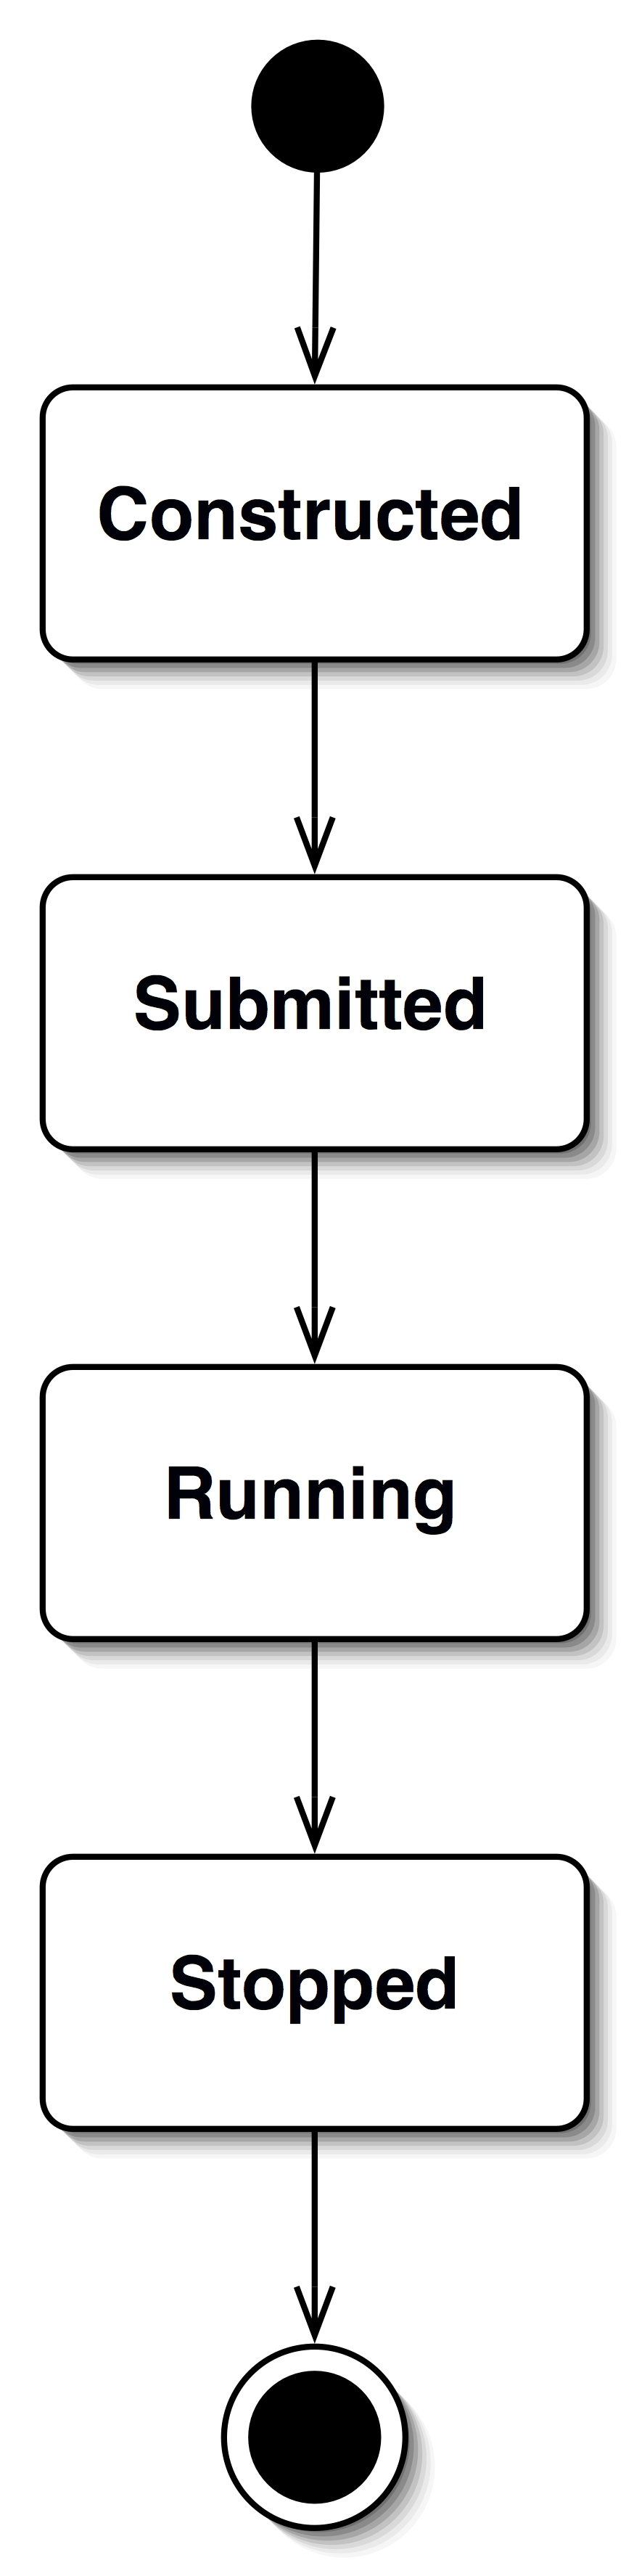
\includegraphics{SimpleJob}
\end{center}      
\caption{A state diagram for an instance of the class SimpleJob.}
\label{Fig:SimpleJobStateDiagram}
\end{figure}

In addition a SimpleJob allows one or more Metrics to be monitored.

%%%%%%%%%%%%%%%%%%%%%%%%%%%%%%%%%%%%%%%%%%%%%%%%%%%%%%%%%%%%%%%%%%%%%%%%%%%%%%%%

\subsubsection{Methods}

\paragraph{Constructor}

Constructs a SimpleJob instance corresponding to the passed
SoftwareResourceDescription and GATContext\\

\textit{Parameters}:
\begin{itemize}
\item[] GATContext --- A GATContext used to broker resources
\item[] SoftwareResourceDescription --- A SoftwareResourceDescription describing the simple job's executable
\end{itemize}

 \textit{Throws}:
 \begin{itemize}
 \item[] java.lang.Exception --- Thrown upon creation problems 
 \end{itemize}

\paragraph{Constructor}

Constructs a SimpleJob instance corresponding to the passed
SoftwareResourceDescription and GATContext\\

\textit{Parameters}:
\begin{itemize}
\item[] GATContext --- A GATContext used to broker resources
\item[] SoftwareResourceDescription --- An SoftwareResourceDescription describing the simple job's executable
\item[] Preferences --- A Preferences the preferences for this instance
\end{itemize}

\paragraph{public boolean Equals}

 Tests this SimpleJob for equality with the passed Object. \\

 If the given object is not a SimpleJob, then this method immediately  returns false. \\
 
 If the given object is a SimpleJob then it is deemed equal if it refers to the same instance in memory. \\

 \textit{Parameters}:
 \begin{itemize}
 \item[] Object --- The Object to test for equality 
 \end{itemize}
 
 \textit{Returns}:
\begin{itemize}
\item[] A boolean indicating equality
\end{itemize}

\paragraph{public void Submit}

Submits the associated physical job to a job queue, an ordered list of
jobs which will eventually be run. Eventually the associated physical
job will be taken off of the job queue and begin running. This method
can only be called on a SimpleJob in the Constructed or Stopped state or 
an error will occur. \\

 \textit{Throws}:
 \begin{itemize}
 \item[] java.rmi.RemoteException --- Thrown upon problems accessing the remote instance
 \end{itemize}
 
\textit{Throws}:
\begin{itemize}
\item[] java.io.IOException --- Upon non-remote IO problem 
\end{itemize}

\paragraph{public void Stop}

Stops the associated physical job. Upon a successful call to this
method the associated physical job is forcibly terminated. This method
can only be called on a SimpleJob in the Running state. \\

 \textit{Throws}:
 \begin{itemize}
 \item[] java.rmi.RemoteException --- Thrown upon problems accessing the remote instance 
 \end{itemize}
 
\textit{Throws}:
\begin{itemize}
\item[] java.io.IOException --- Upon non-remote IO problem 
\end{itemize}

\paragraph{public int GetState}

This method returns the state of the associated SimpleJob. This is one
of the associated public member member variables Constructed,
Submitted, Running, or Stopped. \\

 \textit{Returns}:
 \begin{itemize}
 \item[] This method returns the state of the associated SimpleJob, one of the associated member variables
 \end{itemize} 

 \textit{Throws}:
 \begin{itemize}
 \item[] java.rmi.RemoteException --- Thrown upon problems accessing the remote instance 
 \end{itemize}
 
\textit{Throws}:
\begin{itemize}
\item[] java.io.IOException --- Upon non-remote IO problem 
\end{itemize}

\paragraph{public java.util.Map GetInfo}

This method returns an instance of the class java.util.Map which contains
information about the associated SimpleJob. This java.util.Map contains a
set of key/value pairs the key, a java.lang.String, being the name of the
information and the value being the value of the associated named
information.  The minimum set of keys which the returned java.util.Map
contains is as follows:

\begin{itemize}
  \item \textbf{hostname}
  \item \textbf{submissiontime}
  \item \textbf{starttime}
  \item \textbf{stoptime}
\end{itemize}
\paragraph{hostname} 

The key hostname corresponds to a java.lang.String value which is the
name of the host on which the physical job is running, if SimpleJob is
in the Running state, or will be running on, if SimpleJob is in the
Submitted state. If the associated SimpleJob is not in the Running or
Submitted state, then the value is null.

\paragraph{submissiontime} 

The key submissiontime corresponds to a long value which is
the number of milliseconds after January 1, 1970, 00:00:00 GMT when
the associated physical job was submitted. This value is null for a
SimpleJob in the Constructed state otherwise it is not null.

\paragraph{starttime} 

The key starttime corresponds to a long value which is the
number of milliseconds after January 1, 1970, 00:00:00 GMT when the
associated physical job was started. This value is null for a
SimpleJob in the Submitted or Constructed states otherwise it is not
null.

\paragraph{stoptime} 

The key stoptime corresponds to a long value which is the
number of milliseconds after January 1, 1970, 00:00:00 GMT when the
associated physical job stopped. This value is not null for a
SimpleJob in the Stopped state otherwise it is null. \\

Other key/value pairs will be in future added to the list of key/value
pairs returned in this java.util.Map as the need develops. \\

 \textit{Returns}:
 \begin{itemize}
 \item[] An instance of the class java.util.Map which presents information about the associated SimpleJob.
 \end{itemize} 

 \textit{Throws}:
 \begin{itemize}
 \item[] java.rmi.RemoteException --- Thrown upon problems accessing the remote instance 
 \end{itemize}
 
 \textit{Throws}:
\begin{itemize}
\item[] java.io.IOException --- Upon non-remote IO problem 
\end{itemize}
 
  \paragraph{GetJobID}
 
 This method returns the job id, a globally unique identifier for the physical
 job corresponding to this instance. This method should be called on an instance
 of this class only when the instance is in a Running or Submitted state or an
 error will be returned. 
 
  \textit{Returns}:
 \begin{itemize}
 \item[] An instance of the class java.lang.String which represents the job ID
 \end{itemize}
 
  \textit{Throws}:
 \begin{itemize}
 \item[] java.rmi.RemoteException --- Thrown upon problems accessing the remote instance 
 \end{itemize}
 
\textit{Throws}:
\begin{itemize}
\item[] java.io.IOException --- Upon non-remote IO problem 
\end{itemize}

%%%%%%%%%%%%%%%%%%%%%%%%%%%%%%%%%%%%%%%%%%%%%%%%%%%%%%%%%%%%%%%%%%%%%%%%%%%%%%%%

\subsubsection{Attributes}

\paragraph{Constructed} --- Constant used to determine the state of an instance of this class. \\

\paragraph{Submitted} --- Constant used to determine the state of an instance of this class. \\

\paragraph{Running} --- Constant used to determine the state of an instance of this class. \\

\paragraph{Stopped} --- Constant used to determine the state of an instance of this class. \\

%%%%%%%%%%%%%%%%%%%%%%%%%%%%%%%%%%%%%%%%%%%%%%%%%%%%%%%%%%%%%%%%%%%%%%%%%%%%%%%%
%%%%%%%%%%%%%%%%%%%%%%%%%%%%%%%%%%%%%%%%%%%%%%%%%%%%%%%%%%%%%%%%%%%%%%%%%%%%%%%%

\newpage

\subsection{public abstract class SimpleJobCpi implements Monitorable}

%%%%%%%%%%%%%%%%%%%%%%%%%%%%%%%%%%%%%%%%%%%%%%%%%%%%%%%%%%%%%%%%%%%%%%%%%%%%%%%%

\subsubsection{Description}

Capability provider interface to the SimpleJob class.

Capability provider wishing to provide the functionality of the SimpleJob class must extend this class and
implement all of the abstract methods in this class. Each abstract method in this class mirrors the
corresponding method in this SimpleJob class and will be used to implement the corresponding method in
the SimpleJob class at runtime. 

%%%%%%%%%%%%%%%%%%%%%%%%%%%%%%%%%%%%%%%%%%%%%%%%%%%%%%%%%%%%%%%%%%%%%%%%%%%%%%%%

\subsubsection{Methods}

\paragraph{Constructor}

Constructs a SimpleJobCpi instance corresponding to the passed
SoftwareResourceDescription and GATContext\\

\textit{Parameters}:
\begin{itemize}
\item[] GATContext --- A GATContext used to broker resources
\item[] SoftwareResourceDescription --- An SoftwareResourceDescription describing the simple job's executable
\end{itemize}

\paragraph{public void Submit}

Submits the associated physical job to a job queue, an ordered list of
jobs which will eventually be run. Eventually the associated physical
job will be taken off of the job queue and begin running. This method
can only be called on a SimpleJobCpi in the Constructed or Stopped state or 
an error will occur. \\

 \textit{Throws}:
 \begin{itemize}
 \item[] java.rmi.RemoteException --- Thrown upon problems accessing the remote instance 
 \end{itemize}
 
\textit{Throws}:
\begin{itemize}
\item[] java.io.IOException --- Upon non-remote IO problem 
\end{itemize}

\paragraph{public void Stop}

Stops the associated physical job. Upon a successful call to this
method the associated physical job is forcibly terminated. This method
can only be called on a SimpleJobCpi in the Running state. \\

 \textit{Throws}:
 \begin{itemize}
 \item[] java.rmi.RemoteException --- Thrown upon problems accessing the remote instance 
 \end{itemize}
 
\textit{Throws}:
\begin{itemize}
\item[] java.io.IOException --- Upon non-remote IO problem 
\end{itemize}

\paragraph{public int GetState}

This method returns the state of the associated SimpleJobCpi. This is one
of the associated public member member variables Constructed,
Submitted, Running, or Stopped. \\

 \textit{Returns}:
 \begin{itemize}
 \item[] This method returns the state of the associated SimpleJobCpi, one of the associated member variables
 \end{itemize} 

 \textit{Throws}:
 \begin{itemize}
 \item[] java.rmi.RemoteException --- Thrown upon problems accessing the remote instance 
 \end{itemize}
 
\textit{Throws}:
\begin{itemize}
\item[] java.io.IOException --- Upon non-remote IO problem 
\end{itemize} 

\paragraph{public java.util.Map GetInfo}

This method returns an instance of the class java.util.Map which contains
information about the associated SimpleJobCpi. This java.util.Map contains a
set of key/value pairs the key, a java.lang.String, being the name of the
information and the value being the value of the associated named
information.  The minimum set of keys which the returned java.util.Map
contains is as follows:

\begin{itemize}
  \item \textbf{hostname}
  \item \textbf{submissiontime}
  \item \textbf{starttime}
  \item \textbf{stoptime}
\end{itemize}
\paragraph{hostname} 

The key hostname corresponds to a java.lang.String value which is the
name of the host on which the physical job is running, if SimpleJobCpi is
in the Running state, or will be running on, if SimpleJobCpi is in the
Submitted state. If the associated SimpleJobCpi is not in the Running or
Submitted state, then the value is null.

\paragraph{submissiontime} 

The key submissiontime corresponds to a long value which is
the number of milliseconds after January 1, 1970, 00:00:00 GMT when
the associated physical job was submitted. This value is null for a
SimpleJobCpi in the Constructed state otherwise it is not null.

\paragraph{starttime} 

The key starttime corresponds to a long value which is the
number of milliseconds after January 1, 1970, 00:00:00 GMT when the
associated physical job was started. This value is null for a
SimpleJobCpi in the Submitted or Constructed states otherwise it is not
null.

\paragraph{stoptime} 

The key stoptime corresponds to a long value which is the
number of milliseconds after January 1, 1970, 00:00:00 GMT when the
associated physical job stopped. This value is not null for a
SimpleJobCpi in the Stopped state otherwise it is null. \\

Other key/value pairs will be in future added to the list of key/value
pairs returned in this java.util.Map as the need develops. \\

 \textit{Returns}:
 \begin{itemize}
 \item[] An instance of the class java.util.Map which presents information about the associated SimpleJobCpi.
 \end{itemize} 

 \textit{Throws}:
 \begin{itemize}
 \item[] java.rmi.RemoteException --- Thrown upon problems accessing the remote instance 
 \end{itemize}

\textit{Throws}:
\begin{itemize}
\item[] java.io.IOException --- Upon non-remote IO problem 
\end{itemize}

%%%%%%%%%%%%%%%%%%%%%%%%%%%%%%%%%%%%%%%%%%%%%%%%%%%%%%%%%%%%%%%%%%%%%%%%%%%%%%%%

\subsubsection{Attributes}

SimpleJobCpi has no publicly available member variables. Use the SimpleJob member variables for state
information. 


%%%%%%%%%%%%%%%%%%%%%%%%%%%%%%%%%%%%%%%%%%%%%%%%%%%%%%%%%%%%%%%%%%%%%%%%%%%%%%%%
%%%%%%%%%%%%%%%%%%%%%%%%%%%%%%%%%%%%%%%%%%%%%%%%%%%%%%%%%%%%%%%%%%%%%%%%%%%%%%%%

\newpage

\subsection{public class CheckpointableSimpleJob extends SimpleJob}

%%%%%%%%%%%%%%%%%%%%%%%%%%%%%%%%%%%%%%%%%%%%%%%%%%%%%%%%%%%%%%%%%%%%%%%%%%%%%%%%

\subsubsection{Description}

An instance of this class represents a checkpointable, monitorable
simple job, a job which requires the start of a single executable and
is checkpointable and monitorable.\\

A checkpointable simple job is what one normally considers when
referring to a starting a program that is checkpointable. Thus, a
simple job is primarily described by the checkpointable software which
is to execute during this checkpointable simple job. The description
of the checkpointable software which is to execute during this simple
job is given by an instance of the class
SoftwareResourceDescription. As detailed in the description section of
the documentation for the class SoftwareResourceDescription, an
instance of the class SoftwareResourceDescription describes a software
component. SimpleJob uses this description to describe the
checkpointable software which is to execute during this checkpointable
simple job. \\

Upon creating an instance of the class CheckpointableSimpleJob the
associated physical job is not immediately running. An instance of the
class CheckpointableSimpleJob has various states which it can be in,
only one of which maps to a running physical job. In particular the
various state are as follows

\begin{itemize}
  \item \textbf{Constructed}
  \item \textbf{Submitted}
  \item \textbf{Running}
  \item \textbf{Checkpointing}
  \item \textbf{Stopped}
\end{itemize}
A description of the various states diagrammed in figure \ref{Fig:CheckpointableSimpleJobStateDiagram} 
is as follows:

\paragraph{Constructed} 

An instance of the class CheckpointableSimpleJob has been constructed,
but the method Submit has not yet been successfully called on this
instance.

\paragraph{Submitted} 

The method Submit has been successfully called on an instance of
CheckpointableSimpleJob while the instance was in the Constructed or
Stopped state.

\paragraph{Running} 

The physical job corresponding to an instance of a
CheckpointableSimpleJob is running.

\paragraph{Checkpointing} 

The physical job corresponding to an instance of a
CheckpointableSimpleJob is running and checkpointing due to a
successful call to the method Checkpoint.

\paragraph{Stopped} 

The physical job corresponding to an instance of a
CheckpointableSimpleJob was running but is not currently running due
to a successful call to the method Stop, or the physical job
corresponding to an instance of a CheckpointableSimpleJob was running
but is not currently running due to the physical job completing. \\

\begin{figure}[h]  
\begin{center}
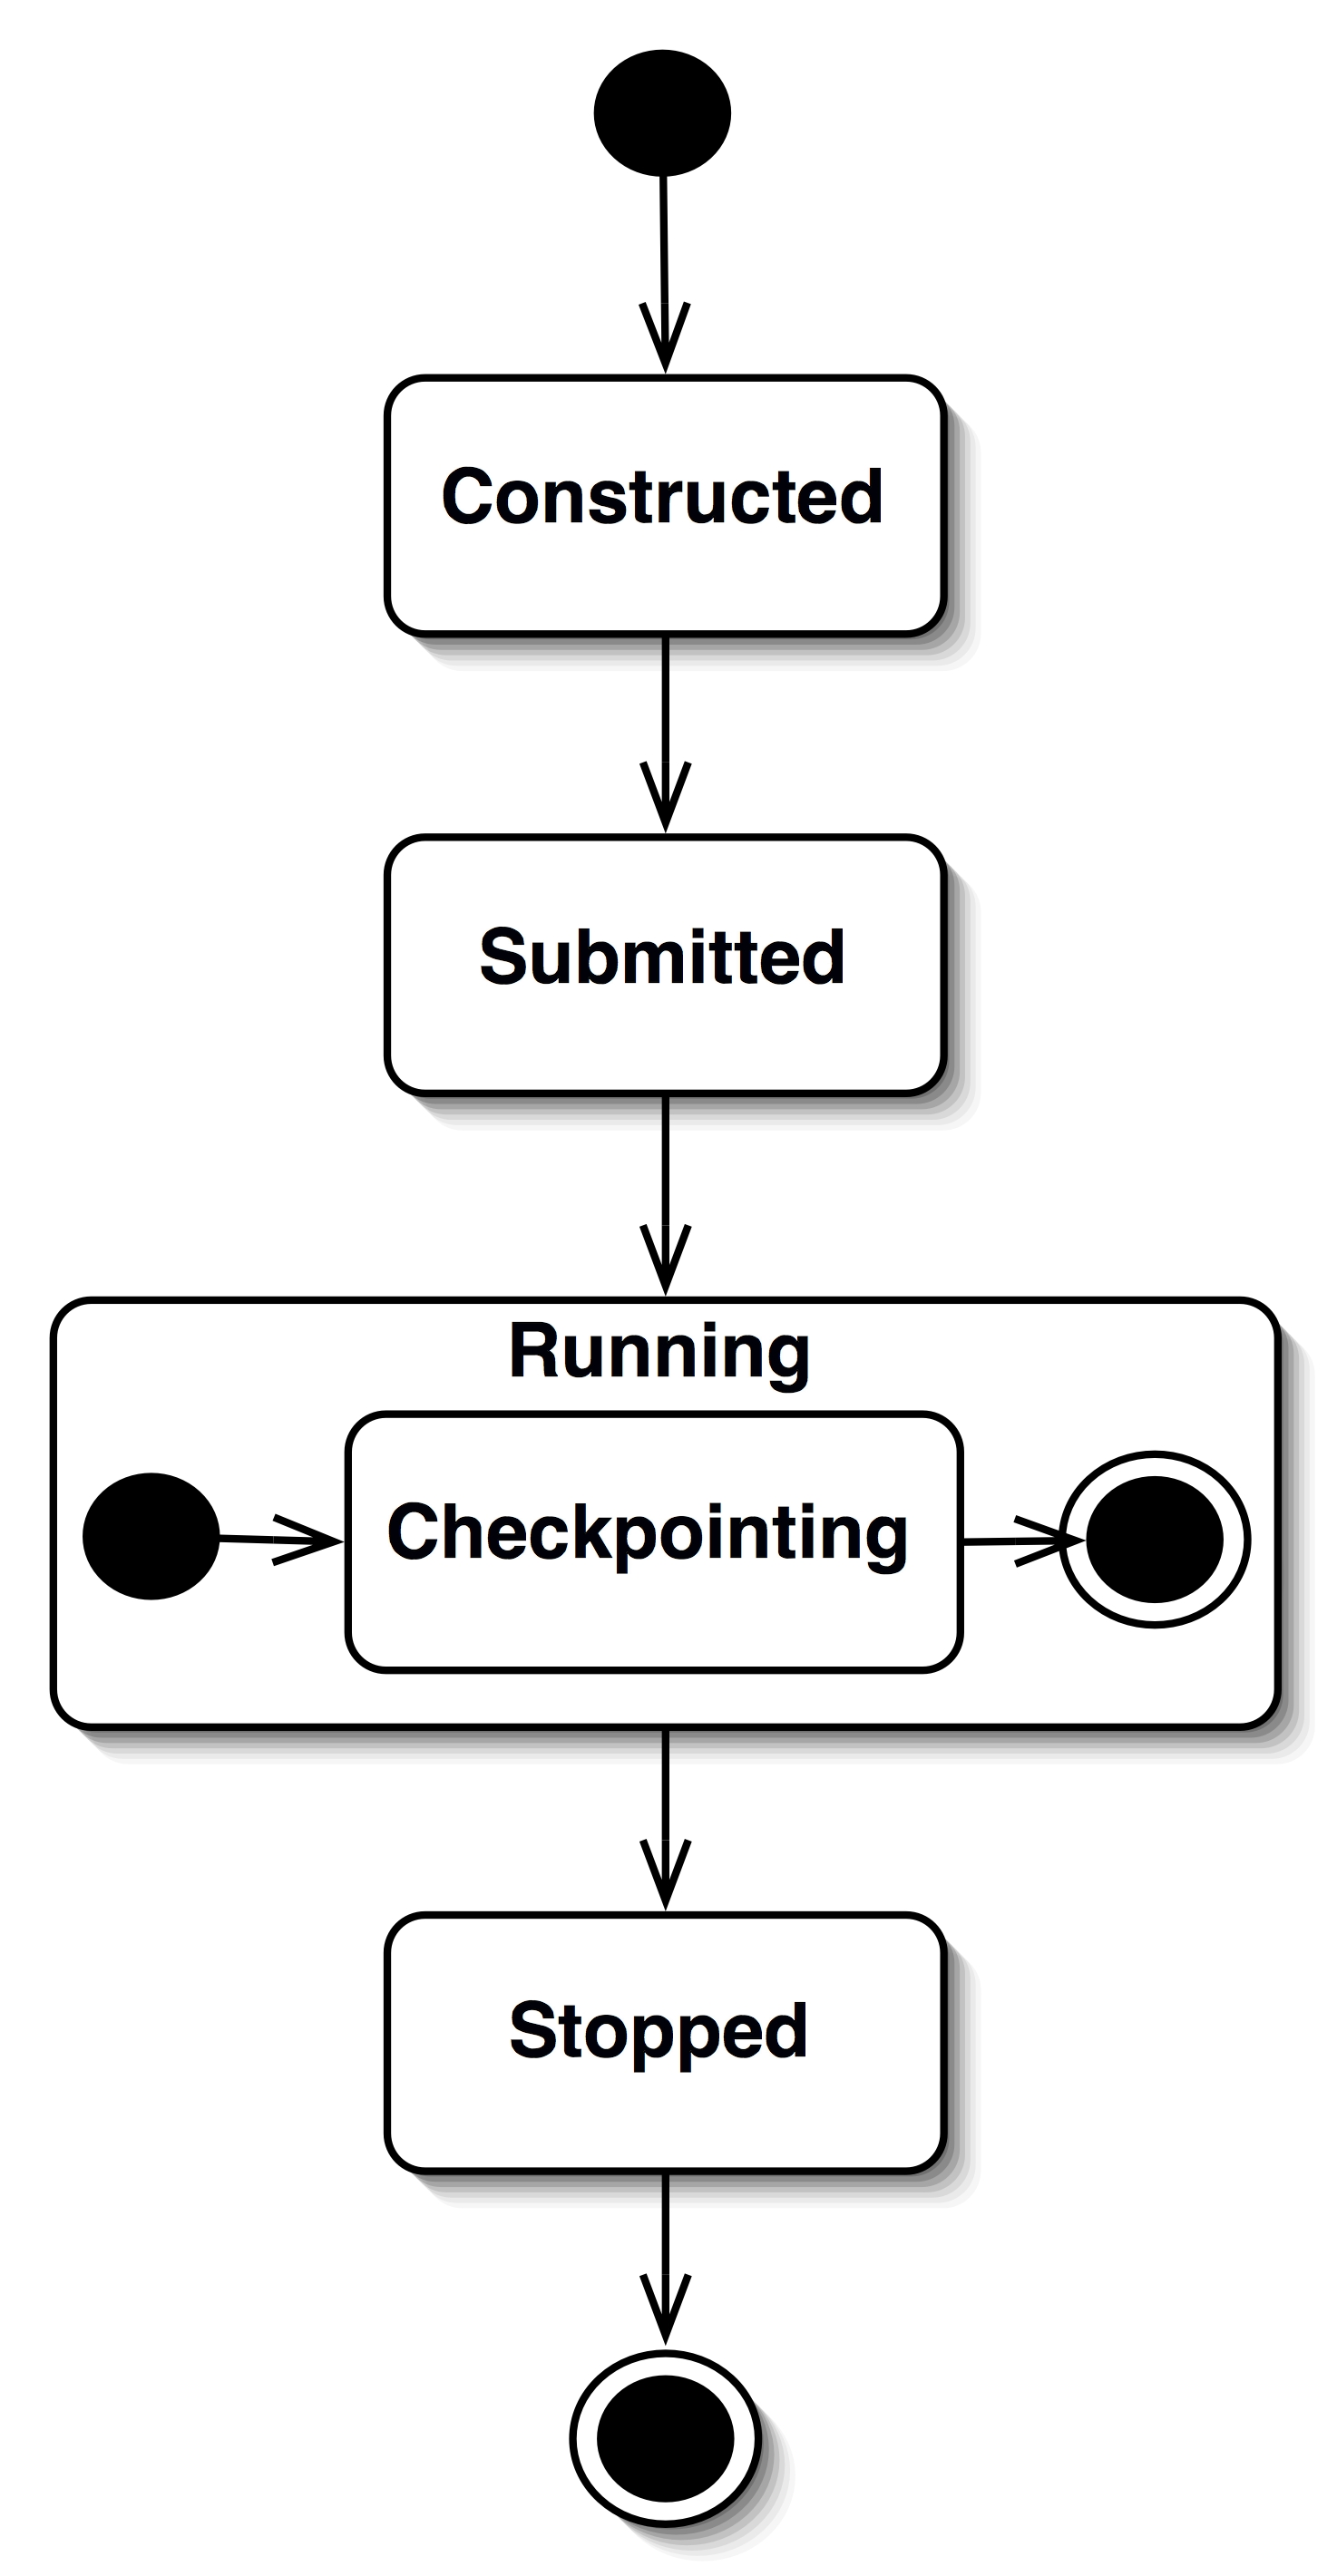
\includegraphics{CheckpointableSimpleJob}
\end{center}      
\caption{A state diagram for an instance of the class CheckpointableSimpleJob.}
\label{Fig:CheckpointableSimpleJobStateDiagram}
\end{figure}

In addition a CheckpointableSimpleJob allows one or more Metrics to be monitored.

%%%%%%%%%%%%%%%%%%%%%%%%%%%%%%%%%%%%%%%%%%%%%%%%%%%%%%%%%%%%%%%%%%%%%%%%%%%%%%%%

\subsubsection{Methods}

\paragraph{Constructor}

Constructs a CheckpointableSimpleJob instance corresponding to the
passed SoftwareResourceDescription and GATContext. \\

\textit{Parameters}:
\begin{itemize}
\item[] SoftwareResourceDescription --- An SoftwareResourceDescription describing the checkpointable 
simple job's executable
\item[] GATContext --- An GATContext used to broker resources
\end{itemize}

\paragraph{Constructor}

Constructs a CheckpointableSimpleJob instance corresponding to the
passed SoftwareResourceDescription and GATContext. \\

\textit{Parameters}:
\begin{itemize}
\item[] SoftwareResourceDescription --- An SoftwareResourceDescription describing the checkpointable 
simple job's executable
\item[] GATContext --- An GATContext used to broker resources
\item[] Preferences --- A Preferences instance used to specify user preferences
\end{itemize}

\paragraph{public boolean Equals}

Tests this CheckpointableSimpleJob for equality with the passed Object. \\

 If the given object is not a CheckpointableSimpleJob, then this
 method immediately returns false. \\
 
 If the given object is a CheckpointableSimpleJob then it is deemed
 equal if it represents the same instance in memory. \\

 \textit{Parameters}:
 \begin{itemize}
 \item[] Object --- The Object to test for equality 
 \end{itemize}
 
 \textit{Returns}:
\begin{itemize}
\item[] A boolean indicating equality
\end{itemize}

\paragraph{public void Checkpoint}

Checkpoints the associated physical job. A physical job is said to be
checkpointed when it writes its current state information to a long
term storage medium. A physical job when checkpointing must write its
current state information to a long term storage medium in such a
manner so that it can, at a later date, by using the state information
stored in the long term storage medium continue running ``from the
same point'' it was at before checkpointing. This is useful for
physical jobs which involve significant data processing and can not,
for any number of reasons, process all of this data in a single run;
also, it is useful for physical jobs which involve significant data
processing and are, for any number of reasons unstable. In both of
these cases checkpointing allows the physical job to process some data
now, then, at a later date, continue running. This method can only be
called on a CheckpointableSimpleJob in the Running state or an error
will occur. \\

 \textit{Throws}:
 \begin{itemize}
 \item[] java.rmi.RemoteException --- Thrown upon problems accessing the remote instance
 \end{itemize}

\textit{Throws}:
\begin{itemize}
\item[] java.io.IOException --- Upon non-remote IO problem 
\end{itemize} 

\paragraph{public void Migrate}

This method is equivalent to calling Checkpoint, Stop, then Submit on
this instance of CheckpointableSimpleJob. \\

 \textit{Throws}:
 \begin{itemize}
 \item[] java.rmi.RemoteException --- Thrown upon problems accessing the remote instance 
 \end{itemize}
 
\textit{Throws}:
\begin{itemize}
\item[] java.io.IOException --- Upon non-remote IO problem 
\end{itemize} 

\paragraph{public void Migrate}

This method is equivalent to calling Checkpoint then Stop on this
instance of CheckpointableSimpleJob, then calling Submit on an
instance of CheckpointableSimpleJob identical to this instance except
that

\begin{itemize}
 \item The CheckpointableSimpleJob when it first enters the Running state will be in the state specified by the 
 state information  stored during the previous call to the Checkpoint method.
 \item The CheckpointableSimpleJob when it first enters the Running state will be running on a hardware 
 resource described in the passed HardwareResourceDescription.
\end{itemize}

 \textit{Parameters}:
 \begin{itemize}
 \item[] HardwareResourceDescription --- A description of the hardware resource to which the physical job
 corresponding to this CheckpointableSimpleJob should be migrated, a HardwareResourceDescription
 \end{itemize}

 \textit{Throws}:
 \begin{itemize}
 \item[] java.rmi.RemoteException --- Thrown upon problems accessing the remote instance 
 \end{itemize}
 
\textit{Throws}:
\begin{itemize}
\item[] java.io.IOException --- Upon non-remote IO problem 
\end{itemize} 

\paragraph{public int GetState}

This method returns the state of the associated
CheckpointableSimpleJob. This is one of the associated public member
member variables Constructed, Submitted, Running,
Checkpointing, or Stopped. \\

 \textit{Returns}:
 \begin{itemize}
 \item[] This method returns the state of the associated CheckpointableSimpleJob one of the associated member
 variables
 \end{itemize} 

 \textit{Throws}:
 \begin{itemize}
 \item[] java.rmi.RemoteException --- Thrown upon problems accessing the remote instance 
 \end{itemize}
 
\textit{Throws}:
\begin{itemize}
\item[] java.io.IOException --- Upon non-remote IO problem 
\end{itemize}

%%%%%%%%%%%%%%%%%%%%%%%%%%%%%%%%%%%%%%%%%%%%%%%%%%%%%%%%%%%%%%%%%%%%%%%%%%%%%%%%

\subsubsection{Attributes}

\paragraph{Checkpointing} --- Constant used to determine the state of an instance of this class.

%%%%%%%%%%%%%%%%%%%%%%%%%%%%%%%%%%%%%%%%%%%%%%%%%%%%%%%%%%%%%%%%%%%%%%%%%%%%%%%%
%%%%%%%%%%%%%%%%%%%%%%%%%%%%%%%%%%%%%%%%%%%%%%%%%%%%%%%%%%%%%%%%%%%%%%%%%%%%%%%%

\newpage

\subsection{public class CheckpointableSimpleJobCpi extends SimpleJobCpi}

%%%%%%%%%%%%%%%%%%%%%%%%%%%%%%%%%%%%%%%%%%%%%%%%%%%%%%%%%%%%%%%%%%%%%%%%%%%%%%%%

\subsubsection{Description}

Capability provider interface to the CheckpointableSimpleJob class.

Capability provider wishing to provide the functionality of the CheckpointableSimpleJob class must extend 
this class and implement all of the abstract methods in this class. Each abstract method in this class 
mirrors the corresponding method in this CheckpointableSimpleJob class and will be used to implement 
the corresponding method in the CheckpointableSimpleJob class at runtime. 

%%%%%%%%%%%%%%%%%%%%%%%%%%%%%%%%%%%%%%%%%%%%%%%%%%%%%%%%%%%%%%%%%%%%%%%%%%%%%%%%

\subsubsection{Methods}

\paragraph{Constructor}

Constructs a CheckpointableSimpleJobCpi instance corresponding to the
passed SoftwareResourceDescription and GATContext. \\

\textit{Parameters}:
\begin{itemize}
\item[] SoftwareResourceDescription --- An SoftwareResourceDescription describing the checkpointable 
simple job's executable
\item[] GATContext --- An GATContext used to broker resources
\end{itemize}

\paragraph{public void Checkpoint}

Checkpoints the associated physical job. A physical job is said to be
checkpointed when it writes its current state information to a long
term storage medium. A physical job when checkpointing must write its
current state information to a long term storage medium in such a
manner so that it can, at a later date, by using the state information
stored in the long term storage medium continue running ``from the
same point'' it was at before checkpointing. This is useful for
physical jobs which involve significant data processing and can not,
for any number of reasons, process all of this data in a single run;
also, it is useful for physical jobs which involve significant data
processing and are, for any number of reasons unstable. In both of
these cases checkpointing allows the physical job to process some data
now, then, at a later date, continue running. This method can only be
called on a CheckpointableSimpleJobCpi in the Running state or an error
will occur. \\

 \textit{Throws}:
 \begin{itemize}
 \item[] java.rmi.RemoteException --- Thrown upon problems accessing the remote instance 
 \end{itemize}

\paragraph{public  void Migrate}

This method is equivalent to calling Checkpoint, Stop, then Submit on
this instance of CheckpointableSimpleJobCpi. \\

 \textit{Throws}:
 \begin{itemize}
 \item[] java.rmi.RemoteException --- Thrown upon problems accessing the remote instance 
 \end{itemize}

\paragraph{public void Migrate}

This method is equivalent to calling Checkpoint then Stop on this
instance of CheckpointableSimpleJobCpi, then calling Submit on an
instance of CheckpointableSimpleJobCpi identical to this instance except
that

\begin{itemize}
 \item The CheckpointableSimpleJobCpi when it first enters the Running state will be in the state specified 
 by the state information  stored during the previous call to the Checkpoint method.
 \item The CheckpointableSimpleJobCpi when it first enters the Running state will be running on a hardware 
 resource described in the passed HardwareResourceDescription.
\end{itemize}

 \textit{Parameters}:
 \begin{itemize}
 \item[] HardwareResourceDescription --- A description of the hardware resource to which the physical job
 corresponding to this CheckpointableSimpleJobCpi should be migrated, a HardwareResourceDescription
 \end{itemize}

 \textit{Throws}:
 \begin{itemize}
 \item[] java.rmi.RemoteException --- Thrown upon problems accessing the remote instance 
 \end{itemize}

\paragraph{public int GetState}

This method returns the state of the associated
CheckpointableSimpleJobCpi. This is one of the associated public member
member variables Constructed, Submitted, Running,
Running.Checkpointing, or Stopped. \\

 \textit{Returns}:
 \begin{itemize}
 \item[] This method returns the state of the associated CheckpointableSimpleJobCpi one of the associated 
 member variables
 \end{itemize} 

 \textit{Throws}:
 \begin{itemize}
 \item[] java.rmi.RemoteException --- Thrown upon problems accessing the remote instance 
 \end{itemize}

%%%%%%%%%%%%%%%%%%%%%%%%%%%%%%%%%%%%%%%%%%%%%%%%%%%%%%%%%%%%%%%%%%%%%%%%%%%%%%%%

\subsubsection{Attributes}

CheckpointableSimpleJobCpi has no publicly available member variables. Use the CheckpointableSimpleJob
member variables for state information. 

%%%%%%%%%%%%%%%%%%%%%%%%%%%%%%%%%%%%%%%%%%%%%%%%%%%%%%%%%%%%%%%%%%%%%%%%%%%%%%%%
%%%%%%%%%%%%%%%%%%%%%%%%%%%%%%%%%%%%%%%%%%%%%%%%%%%%%%%%%%%%%%%%%%%%%%%%%%%%%%%%

\newpage

\subsection{public class SoftwareResourceDescription}

%%%%%%%%%%%%%%%%%%%%%%%%%%%%%%%%%%%%%%%%%%%%%%%%%%%%%%%%%%%%%%%%%%%%%%%%%%%%%%%%

\subsubsection{Description}

An instance of this class is a description of a software resource, a
logical thing, which a may be required by a hardware or software
component.\\

To clarify the rather vague concept of what is a
SoftwareResourceDescription describes let us give various examples. An
application is described by a SoftwareResourceDescription; a software
library is described by a SoftwareResourceDescription; a helper
application is described by a SoftwareResourceDescription; a plugin is
described a SoftwareResourceDescription\ldots However, a piece of
hardware is not described by a SoftwareResourceDescription. In general
any resource which corresponds to a logical thing is described by a
SoftwareResourceDescription. \\

Software is generally useless without hardware. For example, a
software driver without the appropriate Disk drive is all but
useless. Similarly, software often depends upon other software. For
example, having a Photoshop without any plugins is not of much
use. Hence, in describing a software component one needs to also
describe the software and hardware that this software component
requires. This is reflected in the fact that a
SoftwareResourceDescription contains in addition to a ``parent''
description of a software component a java.util.List of
HardwareResourceDescriptions, each element of which describes a
hardware component upon which the parent software component depends,
and a java.util.List of SoftwareResourceDescriptions, each element of which
describes a software component upon which the parent software
component depends. Hence, the entire structure is recursive. \\

To construct an instance of a SoftwareResourceDescription one requires three quantities:
\begin{itemize}
  \item A java.util.Map which contains a set of name/value pairs, detailed later, which describe a software
   resource.
  \item A java.util.List of SoftwareResourceDescription instances each of which describes a software resource upon
  which the parent software resource depends.
  \item A java.util.List of HardwareResourceDescription instances each of which describes a hardware 
  resource upon which the parent software resource depends.
\end{itemize}

The GAT-API defines a minimum set of supported name/value pairs which
can be included in the java.util.Map used to construct a
SoftwareResourceDescription instance. This minimum set of name/value
pairs MUST be supported by any implementation of the GAT-API. This
minimum set of supported name/values is given in the table
\ref{table:SRD}:

\begin{table}[htp]
\begin{center}
\begin{tabular}{|l|c|l|} \hline
Name & Type & Description \\ \hline\hline
\verb"software.location" & \verb"Location" & The software location. \\ \hline
\verb"software.checkpointable" & \verb"Boolean" & A boolean indicating if the software is checkpointable. \\ \hline
\verb"software.arguments" & \verb"java.util.List" & The software arguments,elements are java.lang.String's. \\ \hline
\verb"software.environment" & \verb"java.util.Map" & The software environment, names/values are java.lang.String's. \\ \hline
\verb"software.stdin" & \verb"File" & The software stdin. \\ \hline
\verb"software.stdout" & \verb"Location" & The software stdout. \\ \hline
\verb"software.stderr" & \verb"Location" & The software stderr. \\ \hline
\verb"os.name" & \verb"java.lang.String" & The os name  as returned from \texttt{uname -s}. \\ \hline
\verb"os.type" & \verb"java.lang.String" & The os type  as returned from \texttt{uname -p}. \\ \hline
\verb"os.version" & \verb"java.lang.String" & The os version  as returned from \texttt{uname -v}. \\ \hline
\verb"os.release" & \verb"java.lang.String" & The os release  as returned from \texttt{uname -r}. \\ \hline
\verb"os.name" & \verb"java.lang.String" & The os name  as returned from \texttt{uname -s}. \\ \hline
\end{tabular}
\end{center}
\caption{This minimum set of supported name/values.}
\label{table:SRD}
\end{table}

%%%%%%%%%%%%%%%%%%%%%%%%%%%%%%%%%%%%%%%%%%%%%%%%%%%%%%%%%%%%%%%%%%%%%%%%%%%%%%%%

\subsubsection{Methods}

\paragraph{Constructor}

Constructs a SoftwareResourceDescription associated with the passed objects:
\begin{itemize}
  \item \textbf{SoftwareResourceDescription} --- A java.util.Map, which describes the ``parent'' software
  component.
  \item \textbf{SoftwareResourceDescriptions} --- A java.util.List, which is a list of SoftwareResourceDescriptions
  each of which describes a software component upon which the ``parent'' software component depends.
  \item \textbf{HardwareResourceDescriptions} --- A java.util.List, which is a list of HardwareResourceDescriptions
  each of which describes a hardware component upon which the ``parent'' software component depends.\\
\end{itemize}

\textit{Parameters}:
\begin{itemize}
\item[] SoftwareResourceDescription --- A java.util.Map, which describes the ``parent'' software component.
\item[] SoftwareResourceDescriptions --- A java.util.List, which is a list of SoftwareResourceDescriptions each of which
 describes a software component upon which the ``parent'' software component depends.
 \item[] HardwareResourceDescriptions --- A java.util.List, which is a list of HardwareResourceDescriptions
  each of which describes a hardware component upon which the ``parent'' software component depends.\\
\end{itemize}

\paragraph{public boolean Equals}

Tests this SoftwareResourceDescription for equality with the passed
Object. \\

 If the given object is not a SoftwareResourceDescription, then this
 method immediately returns false. \\
 
 If the passed object is a SoftwareResourceDescription, then it is
 deemed equal if it has an equivalent SoftwareResourceDescription, as
 determined by the Equals method on java.util.Map, and an equivalent
 SoftwareResourceDescriptions, as determined by the Equals method on
 java.util.List, and an equivalent HardwareResourceDescriptions, as determined
 by the Equals method on java.util.List. \\
 
 % Note: As List is now language dependent we have to be explicit here!!!
 
\textit{Parameters}:
\begin{itemize}
\item[] Object --- The Object to test for equality 
\end{itemize}

\textit{Returns}:
\begin{itemize}
\item[] A boolean indicating equality
\end{itemize}
 
\paragraph{public void AddSoftwareResourceAttribute}

Adds the name/value pair to the java.util.Map of name/value pairs which
describe the ``parent'' software component. \\

\textit{Parameters}:
\begin{itemize}
\item[] Name --- The Name, a java.lang.String, to add to the  name/value pairs which describe the ``parent'' 
software component.
\item[] Value --- The Value, an Object, to add to the  name/value pairs which describe the ``parent'' 
software component.
\end{itemize}

\paragraph{public void RemoveSoftwareResourceAttribute}

Removes the name/value pair with the passed name from the java.util.Map of
name/value pairs which describe the ``parent'' software component. \\

\textit{Parameters}:
\begin{itemize}
\item[] Name --- The Name, a java.lang.String, to of the name/value pair to remove from the  name/value pairs 
which describe the ``parent'' software component.
\end{itemize}

\paragraph{public void AddHardwareResourceDescription}

Adds the passed HardwareResourceDescription to the java.util.List of
HardwareResourceDescriptions which describe this
SoftwareResourceDescription. \\

\textit{Parameters}:
\begin{itemize}
\item[] HardwareResourceDescription --- The HardwareResourceDescription to add to the java.util.List of 
HardwareResourceDescriptions which describe this SoftwareResourceDescription.
\end{itemize}
 
\paragraph{public void RemoveHardwareResourceDescription}

Removes the passed HardwareResourceDescription from the java.util.List of
HardwareResourceDescriptions which describe this
SoftwareResourceDescription. \\

\textit{Parameters}:
\begin{itemize}
\item[] HardwareResourceDescription --- The HardwareResourceDescription to remove from the java.util.List of HardwareResourceDescriptions which describe this SoftwareResourceDescription.
\end{itemize}

\paragraph{public void SetHardwareResourceDescriptions}

Sets the java.util.List of HardwareResourceDescriptions which describe this
SoftwareResourceDescription to the passed java.util.List. \\

\textit{Parameters}:
\begin{itemize}
\item[] HardwareResourceDescriptions --- The new java.util.List of HardwareResourceDescriptions which describe 
this SoftwareResourceDescription.
\end{itemize}

\paragraph{public java.util.List GetHardwareResourceDescriptions}

Gets the java.util.List of HardwareResourceDescriptions which describe this
SoftwareResourceDescription. \\

\textit{Returns}:
\begin{itemize}
\item[] The java.util.List of HardwareResourceDescriptions which describe this 
SoftwareResourceDescription.
\end{itemize}

\paragraph{public void AddSoftwareResourceDescription}

Adds the passed SoftwareResourceDescription to the java.util.List of
SoftwareResourceDescriptions which describe this
SoftwareResourceDescription. \\

\textit{Parameters}:
\begin{itemize}
\item[] SoftwareResourceDescription --- The SoftwareResourceDescription to add to the java.util.List of 
SoftwareResourceDescriptions which describe this SoftwareResourceDescription.
\end{itemize}
 
\paragraph{public void RemoveSoftwareResourceDescription}

Removes the passed SoftwareResourceDescription from the java.util.List of
SoftwareResourceDescriptions which describe this
SoftwareResourceDescription. \\

\textit{Parameters}:
\begin{itemize}
\item[] SoftwareResourceDescription --- The SoftwareResourceDescription to remove from the java.util.List 
of SoftwareResourceDescriptions which describe this SoftwareResourceDescription.
\end{itemize}

\paragraph{public void SetSoftwareResourceDescriptions}

Sets the java.util.List of SoftwareResourceDescriptions which describe this
SoftwareResourceDescription to the passed java.util.List. \\

\textit{Parameters}:
\begin{itemize}
\item[] SoftwareResourceDescriptions --- The new java.util.List of SoftwareResourceDescriptions which describe 
this SoftwareResourceDescription.
\end{itemize}

\paragraph{public java.util.List GetSoftwareResourceDescriptions}

Gets the java.util.List of SoftwareResourceDescriptions which describe this SoftwareResourceDescription. \\

\textit{Returns}:
\begin{itemize}
\item[] The java.util.List of SoftwareResourceDescriptions which describe this 
SoftwareResourceDescription.
\end{itemize}

%%%%%%%%%%%%%%%%%%%%%%%%%%%%%%%%%%%%%%%%%%%%%%%%%%%%%%%%%%%%%%%%%%%%%%%%%%%%%%%%

\subsubsection{Attributes}

SoftwareResourceDescription has no publicly available member variables. 

%%%%%%%%%%%%%%%%%%%%%%%%%%%%%%%%%%%%%%%%%%%%%%%%%%%%%%%%%%%%%%%%%%%%%%%%%%%%%%%%
%%%%%%%%%%%%%%%%%%%%%%%%%%%%%%%%%%%%%%%%%%%%%%%%%%%%%%%%%%%%%%%%%%%%%%%%%%%%%%%%

\newpage

\subsection{public abstract class HardwareResourceDescription}

%%%%%%%%%%%%%%%%%%%%%%%%%%%%%%%%%%%%%%%%%%%%%%%%%%%%%%%%%%%%%%%%%%%%%%%%%%%%%%%%

\subsubsection{Description}

An instance of this class is a description of a hardware resource, a
physical thing, which a may be required by a hardware or software
component. \\

To clarify the rather vague concept of what is a
HardwareResourceDescription describes let us give various
examples. Memory is described by a HardwareResourceDescription; a
network is described by a HardwareResourceDescription; disk space is
described by a HardwareResourceDescription; a monitor is described a
HardwareResourceDescription\ldots However, an application is not
described by a HardwareResourceDescription. In general any resource
which corresponds to a physical thing is described by a
HardwareResourceDescription. \\

Hardware is generally useless without software. For example, a disk
drive without the appropriate software driver is all but
useless. Similarly, hardware often depends upon other hardware. For
example, having a disk drive without a computer again is not of much
use. Hence, in describing a hardware component one needs to also
describe the software and hardware that this hardware component
requires. This is reflected in the fact that a
HardwareResourceDescription contains in addition to a description of a
hardware component a java.util.List of HardwareResourceDescriptions, each
element of which describes a hardware component upon which the parent
hardware component depends, and a java.util.List of
SoftwareResourceDescriptions, each element of which describes a
software component upon which the parent hardware component
depends. Hence, the entire structure is recursive. \\

To construct an instance of a HardwareResourceDescription one requires
three quantities:

\begin{itemize}
  \item A java.util.Map which contains a set of name/value pairs, detailed later, which describe a hardware
   resource.
  \item A java.util.List of SoftwareResourceDescription instances each of which describes a software resource upon
  which the parent hardware resource depends.
  \item A java.util.List of HardwareResourceDescription instances each of which describes a hardware resource upon
  which the parent hardware resource depends.
\end{itemize}
The GAT-API defines a minimum set of supported name/value pairs which can be included in the java.util.Map
used to construct a HardwareResourceDescription instance. This minimum set of name/value pairs MUST 
be supported by any implementation of the GAT-API. This minimum set of supported name/values is given
in the table \ref{table:HRD}:
\begin{table}[htp]
\begin{center}
\begin{tabular}{|l|c|l|} \hline
Name & Type & Description \\ \hline\hline
\verb"memory.size" & \verb"Float" & The minimum memory in GB. \\ \hline
\verb"memory.accesstime" & \verb"Float" & The minimum memory access time in ns. \\ \hline
\verb"memory.str" & \verb"Float" & The minimum sustained transfer rate in GB/s. \\ \hline
\verb"machine.type" & \verb"java.lang.String" & The machine type as returned from \texttt{uname -m}. \\ \hline
\verb"machine.node" & \verb"java.lang.String" & The machine node name as returned from \texttt{uname -n}. \\ \hline
\verb"cpu.type" & \verb"java.lang.String" & The generic cpu type as returned from \texttt{uname -p}. \\ \hline
\verb"cpu.speed" & \verb"Float" & The minimum cpu speed in GHz. \\ \hline
\verb"disk.size" & \verb"Float" & The minimum size of the hard drive in GB. \\ \hline
\verb"disk.accesstime" & \verb"Float" & The minimum disk access time in ms. \\ \hline
\verb"disk.str" & \verb"Float" & The minimum sustained transfer rate in MB/s. \\ \hline
\end{tabular}
\end{center}
\caption{This minimum set of supported name/values.}
\label{table:HRD}
\end{table}

%%%%%%%%%%%%%%%%%%%%%%%%%%%%%%%%%%%%%%%%%%%%%%%%%%%%%%%%%%%%%%%%%%%%%%%%%%%%%%%%

\subsubsection{Methods}

\paragraph{Constructor}

Constructs a HardwareResourceDescription associated with the passed objects:
\begin{itemize}
  \item \textbf{HardwareResourceDescription} --- A java.util.Map, which describes the ``parent'' hardware
  component.
  \item \textbf{SoftwareResourceDescriptions} --- A java.util.List, which is a list of SoftwareResourceDescriptions
  each of which describes a software component upon which the ``parent'''' hardware component depends.
  \item \textbf{HardwareResourceDescriptions} --- A java.util.List, which is a list of HardwareResourceDescriptions
  each of which describes a hardware component upon which the ``parent'' hardware component depends.\\
\end{itemize}

\textit{Parameters}:
\begin{itemize}
\item[] HardwareResourceDescription --- A java.util.Map, which describes the ``parent'' hardware component.
\item[] SoftwareResourceDescriptions --- A java.util.List, which is a list of SoftwareResourceDescriptions each of which
 describes a software component upon which the ``parent'' hardware component depends.
 \item[] HardwareResourceDescriptions --- A java.util.List, which is a list of HardwareResourceDescriptions
  each of which describes a hardware component upon which the ``parent'' hardware component depends.\\
\end{itemize}

\paragraph{public boolean Equals}

Tests this HardwareResourceDescription for equality with the passed
Object. \\

 If the given object is not a HardwareResourceDescription, then this
 method immediately returns false. \\
 
 If the passed object is a HardwareResourceDescription, then it is
 deemed equal if it has an equivalent HardwareResourceDescription, as
 determined by the Equals method on java.util.Map, and an equivalent
 SoftwareResourceDescriptions, as determined by the Equals method on
 java.util.List, and an equivalent HardwareResourceDescriptions, as determined
 by the Equals method on java.util.List.
 
 % Note: As List is now language dependent we have to be explicit here!!!
 
\textit{Parameters}:
\begin{itemize}
\item[] Object --- The Object to test for equality 
\end{itemize}

\textit{Returns}:
\begin{itemize}
\item[] A boolean indicating equality
\end{itemize}
 
\paragraph{public void AddHardwareResourceAttribute}

Adds the name/value pair to the java.util.Map of name/value pairs which
describe the ``parent'' hardware component. \\

\textit{Parameters}:
\begin{itemize}
\item[] Name --- The Name, a java.lang.String, to add to the  name/value pairs which describe the ``parent'' 
hardware component.
\item[] Value --- The Value, an Object, to add to the  name/value pairs which describe the ``parent'' 
hardware component.
\end{itemize}

\paragraph{public void RemoveHardwareResourceAttribute}

Removes the name/value pair with the passed name from the java.util.Map of
name/value pairs which describe the ``parent'' hardware component. \\

\textit{Parameters}:
\begin{itemize}
\item[] Name --- The Name, a java.lang.String, to of the name/value pair to remove from the  name/value pairs 
which describe the ``parent'' hardware component.
\end{itemize}

\paragraph{public void AddHardwareResourceDescription}

Adds the passed HardwareResourceDescription to the java.util.List of
HardwareResourceDescriptions which describe this
HardwareResourceDescription. \\

\textit{Parameters}:
\begin{itemize}
\item[] HardwareResourceDescription --- The HardwareResourceDescription to add to the java.util.List of 
HardwareResourceDescriptions which describe this HardwareResourceDescription.
\end{itemize}
 
\paragraph{public void RemoveHardwareResourceDescription}

Removes the passed HardwareResourceDescription from the java.util.List of
HardwareResourceDescriptions which describe this
HardwareResourceDescription. \\

\textit{Parameters}:
\begin{itemize}
\item[] HardwareResourceDescription --- The HardwareResourceDescription
to remove from the java.util.List of HardwareResourceDescriptions which describe
this HardwareResourceDescription.
\end{itemize}

\paragraph{public void SetHardwareResourceDescriptions}

Sets the java.util.List of HardwareResourceDescriptions which describe this
HardwareResourceDescription to the passed java.util.List. \\

\textit{Parameters}:
\begin{itemize}
\item[] HardwareResourceDescriptions --- The new java.util.List of HardwareResourceDescriptions which describe 
this HardwareResourceDescription.
\end{itemize}

\paragraph{public java.util.List GetHardwareResourceDescriptions}

Gets the java.util.List of HardwareResourceDescriptions which describe this
HardwareResourceDescription. \\

\textit{Returns}:
\begin{itemize}
\item[] The java.util.List of HardwareResourceDescriptions which describe this 
HardwareResourceDescription.
\end{itemize}

\paragraph{public void AddSoftwareResourceDescription}

Adds the passed SoftwareResourceDescription to the java.util.List of
SoftwareResourceDescriptions which describe this
HardwareResourceDescription. \\

\textit{Parameters}:
\begin{itemize}
\item[] SoftwareResourceDescription --- The SoftwareResourceDescription to add to the java.util.List of 
SoftwareResourceDescriptions which describe this HardwareResourceDescription.
\end{itemize}
 
\paragraph{public void RemoveSoftwareResourceDescription}

Removes the passed SoftwareResourceDescription from the java.util.List of
SoftwareResourceDescriptions which describe this
HardwareResourceDescription. \\

\textit{Parameters}:
\begin{itemize}
\item[] SoftwareResourceDescription --- The SoftwareResourceDescription to remove from the java.util.List of SoftwareResourceDescriptions which describe this HardwareResourceDescription.
\end{itemize}

\paragraph{public void SetSoftwareResourceDescriptions}

Sets the java.util.List of SoftwareResourceDescriptions which describe this
HardwareResourceDescription to the passed java.util.List. \\

\textit{Parameters}:
\begin{itemize}
\item[] SoftwareResourceDescriptions --- The new java.util.List of SoftwareResourceDescriptions which describe 
this HardwareResourceDescription.
\end{itemize}

\paragraph{public java.util.List GetSoftwareResourceDescriptions}

Gets the java.util.List of SoftwareResourceDescriptions which describe this HardwareResourceDescription. \\

\textit{Returns}:
\begin{itemize}
\item[] The java.util.List of SoftwareResourceDescriptions which describe this 
HardwareResourceDescription.
\end{itemize}


%%%%%%%%%%%%%%%%%%%%%%%%%%%%%%%%%%%%%%%%%%%%%%%%%%%%%%%%%%%%%%%%%%%%%%%%%%%%%%%%

\subsubsection{Attributes}

HardwareResourceDescription has no publicly available member variables.

%%%%%%%%%%%%%%%%%%%%%%%%%%%%%%%%%%%%%%%%%%%%%%%%%%%%%%%%%%%%%%%%%%%%%%%%%%%%%%%%
%%%%%%%%%%%%%%%%%%%%%%%%%%%%%%%%%%%%%%%%%%%%%%%%%%%%%%%%%%%%%%%%%%%%%%%%%%%%%%%%

\newpage

\subsection{public class HardwareResource implements Monitorable}

%%%%%%%%%%%%%%%%%%%%%%%%%%%%%%%%%%%%%%%%%%%%%%%%%%%%%%%%%%%%%%%%%%%%%%%%%%%%%%%%

\subsubsection{Description}

An instance of this class is an abstract representation of a physical
hardware resource which is monitorable.

An instance of this class presents an abstract, system-independent
view of a physical hardware resource which is monitorable. Various
systems use system-dependent means of representing a physical hardware
resource. GAT, however, uses an instance of this class as an operating
system independent description of a physical hardware resource which
is monitorable.

An instance of this class allows on to examine the various properties
of the physical hardware resource to which this instance
corresponds. In addition is allows one to monitor the physical
hardware resource to which this instance corresponds.

%%%%%%%%%%%%%%%%%%%%%%%%%%%%%%%%%%%%%%%%%%%%%%%%%%%%%%%%%%%%%%%%%%%%%%%%%%%%%%%%

\subsubsection{Methods}

\paragraph{public abstract HardwareResourceDescription  GetHardwareResourceDescription}

Gets the HardwareResourceDescription which describes this
HardwareResource instance.

\textit{Returns}:
\begin{itemize}
\item[] A HardwareResourceDescription which describes this HardwareResource instance.
\end{itemize}

%%%%%%%%%%%%%%%%%%%%%%%%%%%%%%%%%%%%%%%%%%%%%%%%%%%%%%%%%%%%%%%%%%%%%%%%%%%%%%%%

\subsubsection{Attributes}

HardwareResource has no publicly available member variables. 

%%%%%%%%%%%%%%%%%%%%%%%%%%%%%%%%%%%%%%%%%%%%%%%%%%%%%%%%%%%%%%%%%%%%%%%%%%%%%%%%
%%%%%%%%%%%%%%%%%%%%%%%%%%%%%%%%%%%%%%%%%%%%%%%%%%%%%%%%%%%%%%%%%%%%%%%%%%%%%%%%

\newpage

\subsection{public interface Streamable}

%%%%%%%%%%%%%%%%%%%%%%%%%%%%%%%%%%%%%%%%%%%%%%%%%%%%%%%%%%%%%%%%%%%%%%%%%%%%%%%%

\subsubsection{Description}

Streamable is a class which provides methods for connections to
external entities such as files or other processes.  There are no
object of this class --- in C++ it might be described as a virtual
class, in Java as an interface.

To send data down a Streamable it is necessary to construct a Buffer, and
pack it with data.  Similarly to receive data a buffer must be created
in which the data will be stored.  Sends and receives may either be
blocking, or asynchronous.  Asynchronous sends or receives must be
completed by an appropriate call.

The method of setting up a connection is the responsibility of the
derived class (e.g. FileStream or Stream).

%%%%%%%%%%%%%%%%%%%%%%%%%%%%%%%%%%%%%%%%%%%%%%%%%%%%%%%%%%%%%%%%%%%%%%%%%%%%%%%%

\subsubsection{Methods}

\paragraph{public void Read}

Reads from this Streamable into the given buffer. 

This is a blocking call and only returns if the buffer is full
or there is no more data to read.\\
 
\textit{Parameters}:
\begin{itemize}
\item[] Buffer --- The Buffer into which data are to be transferred 
\end{itemize}

 \textit{Throws}:
 \begin{itemize}
 \item[] java.io.IOException --- Thrown upon an I/O error of some sort 
 \end{itemize}

\paragraph{public void Write}

Writes data from the given Buffer through the Streamable.  The buffer is not
modified.
 
This is a blocking call and only returns when all the data in the
buffer has been sent.\\

\textit{Parameters}:
\begin{itemize}
\item[] Buffer --- The Buffer from which data are to be transferred 
\end{itemize}

 \textit{Throws}:
 \begin{itemize}
 \item[] java.io.IOException --- Thrown upon an I/O error of some sort 
 \end{itemize}

\paragraph{public void IRead}

Reads from this Streamable into the given buffer, but returning
immediately.  The buffer should not be used until a ReadWait has
been called on this Streamable.

Only one IRead may be active at once on a given Streamable.

This is a non-blocking call.\\
 
\textit{Parameters}:
\begin{itemize}
\item[] Buffer --- The Buffer into which data are to be transferred. 
\end{itemize}

 \textit{Throws}:
 \begin{itemize}
 \item[] java.io.IOException --- Thrown upon an I/O error of some sort 
 \end{itemize}

\paragraph{public boolean ReadFinish}

This finishes the current IRead call on this Streamable.  All data
received between posting the IRead and this call will be available
in the associated buffer on return. \\

\textit{Returns}:
\begin{itemize}
\item[] A boolean indicating if data was received
\end{itemize}

 \textit{Throws}:
 \begin{itemize}
 \item[] java.io.IOException --- Thrown upon an I/O error of some sort 
 \end{itemize}

\paragraph{public boolean ReadTest}

This tests if data has been received in the current IRead.\\

\textit{Returns}:
\begin{itemize}
\item[] A boolean indicating if data was received
\end{itemize}

\paragraph{public void IWrite}

Writes data from the given Buffer through the Streamable, but returning
immediately.  The buffer should not be used until a WriteWait has been
called on this Streamable.  The buffer is not modified, but the position of
the next item in the buffer which would be sent is returned, and this
can be used to remove old data from the buffer.
 
This is a non-blocking call.\\

\textit{Parameters}:
\begin{itemize}
\item[] Buffer --- The Buffer from which data are to be transferred 
\end{itemize}

 \textit{Throws}:
 \begin{itemize}
 \item[] java.io.IOException --- Thrown upon an I/O error of some sort 
 \end{itemize}

\paragraph{public long WriteFinish}

This finishes the current IWrite call on this Streamable.  Not all data in
the buffer may have been sent.\\

\textit{Returns}:
\begin{itemize}
\item[] The position in the buffer right after the last data sent, a long
\end{itemize}

 \textit{Throws}:
 \begin{itemize}
 \item[] java.io.IOException --- Thrown upon an I/O error of some sort 
 \end{itemize}

\paragraph{public long WriteTest}

Tests if data has been sent from  the current IWrite call on this Streamable.\\

\textit{Returns}:
\begin{itemize}
\item[] The position in the buffer right after the last data sent, a long
\end{itemize}

 \textit{Throws}:
 \begin{itemize}
 \item[] java.io.IOException --- Thrown upon an I/O error of some sort 
 \end{itemize}
 
\paragraph{public boolean Equals}

Tests this Streamable for equality with the passed Object.\\

\textit{Parameters}:
\begin{itemize}
\item[] Object --- The Object to test for equality 
\end{itemize}

\textit{Returns}:
\begin{itemize}
\item[] A boolean indicating equality
\end{itemize}

\paragraph{Close}

Closes this Streamable instance. \\

\textit{Throws}:
\begin{itemize}
\item[] java.io.IOException --- Thrown upon an I/O error of some sort 
\end{itemize}

%%%%%%%%%%%%%%%%%%%%%%%%%%%%%%%%%%%%%%%%%%%%%%%%%%%%%%%%%%%%%%%%%%%%%%%%%%%%%%%%

\subsubsection{Attributes}

Streamable has no publicly available member variables. 

%%%%%%%%%%%%%%%%%%%%%%%%%%%%%%%%%%%%%%%%%%%%%%%%%%%%%%%%%%%%%%%%%%%%%%%%%%%%%%%%
%%%%%%%%%%%%%%%%%%%%%%%%%%%%%%%%%%%%%%%%%%%%%%%%%%%%%%%%%%%%%%%%%%%%%%%%%%%%%%%%

\newpage

\subsection{public class Stream implements Monitorable, Streamable}

%%%%%%%%%%%%%%%%%%%%%%%%%%%%%%%%%%%%%%%%%%%%%%%%%%%%%%%%%%%%%%%%%%%%%%%%%%%%%%%%

\subsubsection{Description}

A Stream represents a connection to another process.  It implements
Streamable and the communication methods are derived from that interface.

A Stream represents a streaming connection to another process, and has
semantics similar to the standard BSD socket interface.  Once a Stream
is created it can either be placed in a listening state, or be
connected to a Stream on a remote process.

To send data down a Stream it is necessary to construct a Buffer, and
pack it with data.  Similarly to receive data a buffer must be created
in which the data will be stored.  Sends and receives may either be
blocking, or asynchronous.  Asynchronous sends or receives must be
completed by an appropriate call.  These methods are derived from the
Streamable class.

%%%%%%%%%%%%%%%%%%%%%%%%%%%%%%%%%%%%%%%%%%%%%%%%%%%%%%%%%%%%%%%%%%%%%%%%%%%%%%%%

\subsubsection{Methods}

\paragraph{Constructor}

Constructs a unconnected instance of this class. \\

\textit{Parameters}:
\begin{itemize}
\item[] A GATContext used to broker resources
\end{itemize}

\paragraph{Constructor}

Constructs a unconnected instance of this class. \\

\textit{Parameters}:
\begin{itemize}
\item[] A GATContext used to broker resources
\item[] A Preferences the user preferences for this instance
\end{itemize}

\paragraph{public void Connect}

When a Stream is found, e.g. from a Collection, it is not initially in
a connected state.  The connect method changes the state.

This method takes no parameters.

\textit{Throws}:
\begin{itemize}
\item[] java.io.IOException --- Thrown upon an I/O error of some sort 
\end{itemize}

\paragraph{public Stream Listen}

In order for a connection to be made, a Stream must be set to listen
for connection attempts, and the Stream advertised via a collection.
When a new connection is made, a new Stream is created.

\textit{Returns}:
\begin{itemize}
\item[] A Stream
\end{itemize}

\textit{Throws}:
\begin{itemize}
\item[] java.io.IOException --- Thrown upon an I/O error of some sort 
\end{itemize}

\paragraph{public boolean Equals}

Tests this Stream for equality with the passed Object.\\

If the passed object is not a Stream this method immediately returns false. \\

If the passed object is a Stream it is deemed equivalent if it is the same instance in memory. \\

\textit{Parameters}:
\begin{itemize}
\item[] Object --- The Object to test for equality 
\end{itemize}

\textit{Returns}:
\begin{itemize}
\item[] A boolean indicating equality
\end{itemize}


%%%%%%%%%%%%%%%%%%%%%%%%%%%%%%%%%%%%%%%%%%%%%%%%%%%%%%%%%%%%%%%%%%%%%%%%%%%%%%%%

\subsubsection{Attributes}

Stream has no publicly available member variables. 

%%%%%%%%%%%%%%%%%%%%%%%%%%%%%%%%%%%%%%%%%%%%%%%%%%%%%%%%%%%%%%%%%%%%%%%%%%%%%%%%
%%%%%%%%%%%%%%%%%%%%%%%%%%%%%%%%%%%%%%%%%%%%%%%%%%%%%%%%%%%%%%%%%%%%%%%%%%%%%%%%

\newpage

\subsection{public abstract class StreamCpi implements Monitorable, Streamable}

%%%%%%%%%%%%%%%%%%%%%%%%%%%%%%%%%%%%%%%%%%%%%%%%%%%%%%%%%%%%%%%%%%%%%%%%%%%%%%%%

\subsubsection{Description}

Capability provider interface to the Stream class.

Capability provider wishing to provide the functionality of the Stream class must extend 
this class and implement all of the abstract methods in this class. Each abstract method in this class 
mirrors the corresponding method in this Stream class and will be used to implement 
the corresponding method in the Stream class at runtime. 

%%%%%%%%%%%%%%%%%%%%%%%%%%%%%%%%%%%%%%%%%%%%%%%%%%%%%%%%%%%%%%%%%%%%%%%%%%%%%%%%

\subsubsection{Methods}

\paragraph{Constructor}

Constructs a unconnected instance of this class. \\

\textit{Parameters}:
\begin{itemize}
\item[] A GATContext used to broker resources
\end{itemize}

\paragraph{public void Connect}

When a StreamCpi is found, e.g. from a Collection, it is not initially in
a connected state.  The connect method changes the state.

This method takes no parameters.

\textit{Throws}:
\begin{itemize}
\item[] java.io.IOException --- Thrown upon an I/O error of some sort 
\end{itemize}

\paragraph{public !!! Listen}

In order for a connection to be made, a StreamCpi must be set to listen
for connection attempts, and the StreamCpi advertised via a collection.
When a new connection is made, a new StreamCpi is created, and a callback
or listener (language dependent) is invoked with this new StreamCpi.

The parameters of this method are language dependent.

% !!!

\textit{Throws}:
\begin{itemize}
\item[] java.io.IOException --- Thrown upon an I/O error of some sort 
\end{itemize}

%%%%%%%%%%%%%%%%%%%%%%%%%%%%%%%%%%%%%%%%%%%%%%%%%%%%%%%%%%%%%%%%%%%%%%%%%%%%%%%%

\subsubsection{Attributes}

StreamCpi has no publicly available member variables. 

%%%%%%%%%%%%%%%%%%%%%%%%%%%%%%%%%%%%%%%%%%%%%%%%%%%%%%%%%%%%%%%%%%%%%%%%%%%%%%%%
%%%%%%%%%%%%%%%%%%%%%%%%%%%%%%%%%%%%%%%%%%%%%%%%%%%%%%%%%%%%%%%%%%%%%%%%%%%%%%%%

\newpage

\subsection{public class FileStream implements Monitorable, Streamable}

%%%%%%%%%%%%%%%%%%%%%%%%%%%%%%%%%%%%%%%%%%%%%%%%%%%%%%%%%%%%%%%%%%%%%%%%%%%%%%%%

A FileStream represents a connection to open file, the file may be
either remote or local.  It is derived from the Streamable interface so
some communication functions are as documented there.

A FileStream represents a seekable connection to a file, and has
semantics similar to a standard Unix filedescriptor.  It provides
methods to query the current position in the file and to seek to new positions.

To Write data to a FileStream it is necessary to construct a Buffer,
and pack it with data.  Similarly to read data a buffer must be
created in which the data will be stored.  Since the file may be
remote, writes and reads may either be blocking, or asynchronous.
Asynchronous writes or reads must be completed by appropriate call.
These methods are derived from the Streamable class and are as
documented there.

%%%%%%%%%%%%%%%%%%%%%%%%%%%%%%%%%%%%%%%%%%%%%%%%%%%%%%%%%%%%%%%%%%%%%%%%%%%%%%%%

\subsubsection{Methods}

\paragraph{Constructor}

This creates a FileStream attached to the physical file at the
specified Location.  The file may be opened in several modes:

\begin{itemize}

\item[] FileStream.read --- Open file for reading.  The stream is
positioned at the beginning of the file.

\item[] FileStream.write --- Truncate file to zero length or create file
for writing.  The stream is positioned at the beginning of the file.

\item[] FileStream.readwrite --- Open for reading and writing.  The
stream is positioned at the beginning of the file.

\item[] FileStream.append --- Open for appending (writing at end of
file).  The file is created if it does not exist.  The stream is
positioned at the end of the file.\\

\end{itemize}

\textit{Parameters}:
\begin{itemize}
\item[] GATContext --- The GATContext used to broker resources
\item[] Location --- The Location of the file to open.
\item[] Mode --- The mode to open it --- read, write, readwrite, or append, member variables of this class
\end{itemize}

 \textit{Throws}:
 \begin{itemize}
 \item[] java.lang.Exception --- Thrown upon creation problems 
 \end{itemize}

\paragraph{Constructor}

This creates a FileStream attached to the physical file at the
specified Location.  The file may be opened in several modes:

\begin{itemize}

\item[] FileStream.read --- Open file for reading.  The stream is
positioned at the beginning of the file.

\item[] FileStream.write --- Truncate file to zero length or create file
for writing.  The stream is positioned at the beginning of the file.

\item[] FileStream.readwrite --- Open for reading and writing.  The
stream is positioned at the beginning of the file.

\item[] FileStream.append --- Open for appending (writing at end of
file).  The file is created if it does not exist.  The stream is
positioned at the end of the file.\\

\end{itemize}

\textit{Parameters}:
\begin{itemize}
\item[] GATContext --- The GATContext used to broker resources
\item[] Location --- The Location of the file to open.
\item[] Mode --- The mode to open it --- read, write, readwrite or append, member variables of this class
\item[] Preferences --- The Preferences used to specify user preferences
\end{itemize}

\textit{Throws}:
\begin{itemize}
\item[]  java.io.IOException --- Thrown upon an I/O error of some sort
\end{itemize}

\paragraph{public long Position}

This returns the current position in the file.\\

\textit{Returns}:
\begin{itemize}
\item[] The current position in the file, a long
\end{itemize}

\textit{Throws}:
\begin{itemize}
\item[]  java.io.IOException --- Thrown upon an I/O error of some sort
\end{itemize}

\paragraph{public void Seek}

This changes the current position in the file.  The position can
either be calculated from the current position in the file or from the
beginning or end.\\

\textit{Parameters}:
\begin{itemize}
\item[] Offset --- Offset, a long,  from \bf{whence}.
\item[] Whence --- one of the member variables used for this purpose, beginning, current or end of file.
\end{itemize}

\textit{Throws}:
\begin{itemize}
\item[]  java.io.IOException --- Thrown upon an I/O error of some sort
\end{itemize}

\paragraph{public void Flush}

Make sure that any underlying file-writing mechanisms have flushed
data to disk.

\textit{Throws}:
\begin{itemize}
\item[]  java.io.IOException --- Thrown upon an I/O error of some sort
\end{itemize}

\paragraph{public boolean Equals}

Tests this FileStream for equality with the passed Object.\\

If the passed object is not a FileStream then this method immediately returns false. \\

If the passed object is a FileStream, then it is deemed equivalent if it is the same instance in memory. \\

\textit{Parameters}:
\begin{itemize}
\item[] Object --- The Object to test for equality 
\end{itemize}

\textit{Returns}:
\begin{itemize}
\item[] A boolean indicating equality
\end{itemize}


%%%%%%%%%%%%%%%%%%%%%%%%%%%%%%%%%%%%%%%%%%%%%%%%%%%%%%%%%%%%%%%%%%%%%%%%%%%%%%%%

\subsubsection{Attributes}

\paragraph{read} --- Constant used to indicate read mode

\paragraph{write} --- Constant used to indicate write mode

\paragraph{readwrite} --- Constant used to indicate readwrite mode

\paragraph{append} --- Constant used to indicate append mode

\paragraph{beginning} --- Constant used to indicate seek mode

\paragraph{current} --- Constant used to indicate seek mode

\paragraph{end} --- Constant used to indicate seek mode

%%%%%%%%%%%%%%%%%%%%%%%%%%%%%%%%%%%%%%%%%%%%%%%%%%%%%%%%%%%%%%%%%%%%%%%%%%%%%%%%
%%%%%%%%%%%%%%%%%%%%%%%%%%%%%%%%%%%%%%%%%%%%%%%%%%%%%%%%%%%%%%%%%%%%%%%%%%%%%%%%

\newpage

\subsection{public class FileStreamCpi implements Monitorable, Streamable}

%%%%%%%%%%%%%%%%%%%%%%%%%%%%%%%%%%%%%%%%%%%%%%%%%%%%%%%%%%%%%%%%%%%%%%%%%%%%%%%%

Capability provider interface to the FileStream class.

Capability provider wishing to provide the functionality of the FileStream class must extend 
this class and implement all of the abstract methods in this class. Each abstract method in this class 
mirrors the corresponding method in this FileStream class and will be used to implement 
the corresponding method in the FileStream class at runtime. 

%%%%%%%%%%%%%%%%%%%%%%%%%%%%%%%%%%%%%%%%%%%%%%%%%%%%%%%%%%%%%%%%%%%%%%%%%%%%%%%%

\subsubsection{Methods}

\paragraph{Constructor}

This creates a FileStreamCpi attached to the physical file at the
specified Location.  The file may be opened in several modes:

\begin{itemize}

\item[] FileStream.read --- Open file for reading.  The stream is
positioned at the beginning of the file.

\item[] FileStream.write --- Truncate file to zero length or create file
for writing.  The stream is positioned at the beginning of the file.

\item[] FileStream.readwrite --- Open for reading and writing.  The
stream is positioned at the beginning of the file.

\item[] FileStream.append --- Open for appending (writing at end of
file).  The file is created if it does not exist.  The stream is
positioned at the end of the file.\\

\end{itemize}

\textit{Parameters}:
\begin{itemize}
\item[] GATContext --- The GATContext used to broker resources
\item[] Location --- The Location of the file to open.
\item[] Mode --- The mode to open it --- read, write, readwrite, or append, member variables of the FileStream class
\end{itemize}

\paragraph{public abstract long Position}

This returns the current position in the file.\\

\textit{Returns}:
\begin{itemize}
\item[] The current position in the file, a long
\end{itemize}

\textit{Throws}:
\begin{itemize}
\item[]  java.io.IOException --- Thrown upon an I/O error of some sort
\end{itemize}

\paragraph{public abstract void Seek}

This changes the current position in the file.  The position can
either be calculated from the current position in the file or from the
beginning or end.\\

\textit{Parameters}:
\begin{itemize}
\item[] Offset --- Offset, a long,  from \bf{whence}.
\item[] Whence --- one of the member variables used for this purpose, beginning, current or end of file.
\end{itemize}

\textit{Throws}:
\begin{itemize}
\item[]  java.io.IOException --- Thrown upon an I/O error of some sort
\end{itemize}

\paragraph{public abstract void Flush}

Make sure that any underlying file-writing mechanisms have flushed
data to disk.

\textit{Throws}:
\begin{itemize}
\item[]  java.io.IOException --- Thrown upon an I/O error of some sort
\end{itemize}


%%%%%%%%%%%%%%%%%%%%%%%%%%%%%%%%%%%%%%%%%%%%%%%%%%%%%%%%%%%%%%%%%%%%%%%%%%%%%%%%

\subsubsection{Attributes}

FileStreamCpi has no publicly available member variables. Use the member variables of FileStream for the
mode information. 

%%%%%%%%%%%%%%%%%%%%%%%%%%%%%%%%%%%%%%%%%%%%%%%%%%%%%%%%%%%%%%%%%%%%%%%%%%%%%%%%
%%%%%%%%%%%%%%%%%%%%%%%%%%%%%%%%%%%%%%%%%%%%%%%%%%%%%%%%%%%%%%%%%%%%%%%%%%%%%%%%

\newpage

\subsection{public class ResourceBroker}

%%%%%%%%%%%%%%%%%%%%%%%%%%%%%%%%%%%%%%%%%%%%%%%%%%%%%%%%%%%%%%%%%%%%%%%%%%%%%%%%

\subsubsection{Description}

An instance of this class is used to reserve resources. \\

A resource can either be a hardware resource or a software resource. A
software resource is simply an executable it makes little sense to
reserve such. Thus an instance of this class can currently only reserve a
hardware resource. \\

If one wishes to reserve a hardware resource, one must first describe
the hardware resource that one wishes to reserve. This is accomplished
by creating an instance of the class HardwareResourceDescription which
describes the hardware resource that one wishes to reserve. After
creating such an instance of the class HardwareResourceDescription
that describes the hardware resource one wishes to reserve, one must
specify the time period for which one wishes to reserve the hardware
resource. This is accomplished by creating an instance of the class
TimePeriod which specifies the time period for which one wishes to
reserve the hardware resource. Finally, one must obtain a reservation
for the desired hardware resource for the desired time period. This is
accomplished by calling the method ReserveHardwareResource() on an
instance of the class ResourceBroker with the appropriate instance of
HardwareResourceDescription and the appropriate instance of
TimePeriod. \\

In addition an instance of this class can be used to find hardware resources.
This is accomplished using the method FindHardwareResources(). This is 
accomplished by creating an instance of the class HardwareResourceDescription 
which describes the hardware resource that one wishes to find. After
creating such an instance of the class HardwareResourceDescription
that describes the hardware resource one wishes to find, one must 
find the corresponding hardware resource. This is accomplished by calling the 
method FindHardwareResources() on an instance of the class ResourceBroker 
with the appropriate instance of HardwareResourceDescription. \\

%%%%%%%%%%%%%%%%%%%%%%%%%%%%%%%%%%%%%%%%%%%%%%%%%%%%%%%%%%%%%%%%%%%%%%%%%%%%%%%%

\subsubsection{Methods}

\paragraph{Constructor}

This method constructs a ResourceBroker instance corresponding to the passed GATContext. \\

\textit{Parameters}:
\begin{itemize}
\item[] GATContext --- A GATContext which will be used to broker resources
\end{itemize}

 \textit{Throws}:
 \begin{itemize}
 \item[] java.lang.Exception --- Thrown upon creation problems 
 \end{itemize}
 
\paragraph{Constructor}

This method constructs a ResourceBroker instance corresponding to the passed GATContext. \\

\textit{Parameters}:
\begin{itemize}
\item[] GATContext --- A GATContext which will be used to broker resources
\item[] Preferences --- A Preferences which specifies user preferences
\end{itemize}

 \textit{Throws}:
 \begin{itemize}
 \item[] java.lang.Exception --- Thrown upon creation problems 
 \end{itemize}

\paragraph{public void Equals}

 Tests this ResourceBroker for equality with the passed Object. \\

 If the given object is not a ResourceBroker, then this method immediately returns false. \\
 
 If the passed object is a ResourceBroker, then it is deemed equal if it has an equivalent GATContext, 
 as determined by the Equals method on GATContext. \\
  
\textit{Parameters}:
\begin{itemize}
\item[] Object --- The Object to test for equality 
\end{itemize}

\textit{Returns}:
\begin{itemize}
\item[] A boolean indicating equality
\end{itemize}

\paragraph{public Reservation ReserveHardwareResource}

This method attempts to reserve the specified hardware resource for the specified time period. Upon
reserving the specified hardware resource this method returns a Reservation. Upon failing to 
reserve the specified hardware resource this method returns an error. \\

\textit{Parameters}:
\begin{itemize}
\item[] HardwareResourceDescription --- A description, a HardwareResourceDescription, of the 
hardware resource to reserve
\item[] TimePeriod --- The time period, a TimePeriod , for which to reserve the hardware resource 
\end{itemize}

\textit{Returns}:
\begin{itemize}
\item[] A Reservation upon success 
\end{itemize}

 \textit{Throws}:
 \begin{itemize}
 \item[] java.rmi.RemoteException --- Thrown upon problems accessing the remote instance 
 \end{itemize}
 
\textit{Throws}:
\begin{itemize}
\item[] java.io.IOException --- Upon non-remote IO problem 
\end{itemize}

\paragraph{public java.util.List FindHardwareResources}

This method attempts to find one or more matching hardware
resources. Upon finding the specified hardware resource(s) this method
returns a java.util.List of HardwareResource instances. Upon failing to find the
specified hardware resource this method returns an error. \\

\textit{Parameters}:
\begin{itemize}
\item[] HardwareResoucreDescription --- A description, a  HardwareResoucreDescription, of the hardware
  resource(s) to find
\end{itemize}

\textit{Returns}:
\begin{itemize}
\item[] java.util.List of HardwareResources upon success
\end{itemize}

 \textit{Throws}:
 \begin{itemize}
 \item[] java.rmi.RemoteException --- Thrown upon problems accessing the remote instance 
 \end{itemize}
 
\textit{Throws}:
\begin{itemize}
\item[] java.io.IOException --- Upon non-remote IO problem 
\end{itemize}   

%%%%%%%%%%%%%%%%%%%%%%%%%%%%%%%%%%%%%%%%%%%%%%%%%%%%%%%%%%%%%%%%%%%%%%%%%%%%%%%%

\subsubsection{Attributes}

ResourceBroker has no publicly available member variables.

%%%%%%%%%%%%%%%%%%%%%%%%%%%%%%%%%%%%%%%%%%%%%%%%%%%%%%%%%%%%%%%%%%%%%%%%%%%%%%%%
%%%%%%%%%%%%%%%%%%%%%%%%%%%%%%%%%%%%%%%%%%%%%%%%%%%%%%%%%%%%%%%%%%%%%%%%%%%%%%%%

\newpage

\subsection{public abstract class ResourceBrokerCpi}

%%%%%%%%%%%%%%%%%%%%%%%%%%%%%%%%%%%%%%%%%%%%%%%%%%%%%%%%%%%%%%%%%%%%%%%%%%%%%%%%

\subsubsection{Description}

Capability provider interface to the ResourceBroker class.

Capability provider wishing to provide the functionality of the ResourceBroker class must extend 
this class and implement all of the abstract methods in this class. Each abstract method in this class 
mirrors the corresponding method in this ResourceBroker class and will be used to implement 
the corresponding method in the ResourceBroker class at runtime. 

%%%%%%%%%%%%%%%%%%%%%%%%%%%%%%%%%%%%%%%%%%%%%%%%%%%%%%%%%%%%%%%%%%%%%%%%%%%%%%%%

\subsubsection{Methods}

\paragraph{Constructor}

This method constructs a ResourceBrokerCpi instance corresponding to the passed GATContext. \\

\textit{Parameters}:
\begin{itemize}
\item[] GATContext --- A GATContext which will be used to broker resources
\end{itemize}

\paragraph{public abstract Reservation ReserveHardwareResource}

This method attempts to reserve the specified hardware resource for the specified time period. Upon
reserving the specified hardware resource this method returns a Reservation. Upon failing to 
reserve the specified hardware resource this method returns an error. \\

\textit{Parameters}:
\begin{itemize}
\item[] HardwareResourceDescription --- A description, a HardwareResourceDescription, of the 
hardware resource to reserve
\item[] TimePeriod --- The time period, a TimePeriod , for which to reserve the hardware resource
\end{itemize}

\textit{Returns}:
\begin{itemize}
\item[] A Reservation upon success 
\end{itemize}

 \textit{Throws}:
 \begin{itemize}
 \item[] java.rmi.RemoteException --- Thrown upon problems accessing the remote instance 
 \end{itemize}

\paragraph{public java.util.List FindHardwareResources}

This method attempts to find one or more matching hardware
resources. Upon finding the specified hardware resource(s) this method
returns a java.util.List of HardwareResource instances. Upon failing to find the
specified hardware resource this method returns an error. \\

\textit{Parameters}:
\begin{itemize}
\item[] HardwareResoucreDescription --- A description, a  HardwareResoucreDescription, of the hardware
  resource(s) to find
\end{itemize}

\textit{Returns}:
\begin{itemize}
\item[] java.util.List of HardwareResources upon success
\end{itemize}

 \textit{Throws}:
 \begin{itemize}
 \item[] java.rmi.RemoteException --- Thrown upon problems accessing the remote instance 
 \end{itemize}

%%%%%%%%%%%%%%%%%%%%%%%%%%%%%%%%%%%%%%%%%%%%%%%%%%%%%%%%%%%%%%%%%%%%%%%%%%%%%%%%

\subsubsection{Attributes}

ResourceBrokerCpi has no publicly available member variables.

%%%%%%%%%%%%%%%%%%%%%%%%%%%%%%%%%%%%%%%%%%%%%%%%%%%%%%%%%%%%%%%%%%%%%%%%%%%%%%%%
%%%%%%%%%%%%%%%%%%%%%%%%%%%%%%%%%%%%%%%%%%%%%%%%%%%%%%%%%%%%%%%%%%%%%%%%%%%%%%%%

\newpage

\subsection{public abstract class Reservation}

%%%%%%%%%%%%%%%%%%%%%%%%%%%%%%%%%%%%%%%%%%%%%%%%%%%%%%%%%%%%%%%%%%%%%%%%%%%%%%%%

\subsubsection{Description} 

An instance of this class represents a reservation for resources. \\

%%%%%%%%%%%%%%%%%%%%%%%%%%%%%%%%%%%%%%%%%%%%%%%%%%%%%%%%%%%%%%%%%%%%%%%%%%%%%%%%

\subsubsection{Methods}

\paragraph{public abstract boolean Cancel}

This method upon successfully completing cancels the reservation corresponding to the associated 
Reservation instance. \\

 \textit{Throws}:
 \begin{itemize}
 \item[] java.rmi.RemoteException --- Thrown upon problems accessing the remote instance 
 \end{itemize}
 
 \textit{Throws}:
\begin{itemize}
\item[] java.io.IOException --- Upon non-remote IO problem 
\end{itemize}    

%%%%%%%%%%%%%%%%%%%%%%%%%%%%%%%%%%%%%%%%%%%%%%%%%%%%%%%%%%%%%%%%%%%%%%%%%%%%%%%%

\subsubsection{Attributes}

Reservation has no publicly available member variables.

%%%%%%%%%%%%%%%%%%%%%%%%%%%%%%%%%%%%%%%%%%%%%%%%%%%%%%%%%%%%%%%%%%%%%%%%%%%%%%%%
%%%%%%%%%%%%%%%%%%%%%%%%%%%%%%%%%%%%%%%%%%%%%%%%%%%%%%%%%%%%%%%%%%%%%%%%%%%%%%%%

\newpage

\subsection{public class Collection implements Monitorable}

%%%%%%%%%%%%%%%%%%%%%%%%%%%%%%%%%%%%%%%%%%%%%%%%%%%%%%%%%%%%%%%%%%%%%%%%%%%%%%%%

\subsubsection{Description}

An instance of this class represents a collection, a group of objects
which are known as elements. \\

One can construct a Collection in one of two ways. One can use the no
arguments constructor, which creates an empty collection. One can also
use the constructor which takes a single argument of type Collection,
used creates a new Collection with the same elements as its
argument. In effect, the latter constructor allows the user to copy
any Collection. \\

A Collection instance provides various methods which allow one to add
elements, remove elements, and query the Collection instance. All
elements which are added to a Collection instance must implement the
method Equals(). This allows for one to query the Collection instance
with methods such as Contains() and to remove specific elements with
methods such as Remove().

%%%%%%%%%%%%%%%%%%%%%%%%%%%%%%%%%%%%%%%%%%%%%%%%%%%%%%%%%%%%%%%%%%%%%%%%%%%%%%%%

\subsubsection{Methods}

\paragraph{Constructor}

Constructs an empty Collection.

\textit{Parameters}:
\begin{itemize}
\item[] GATContext --- A GATContext which is used to determine the access rights for this Collection.
\end{itemize}

 \textit{Throws}:
 \begin{itemize}
 \item[] java.lang.Exception --- Thrown upon creation problems 
 \end{itemize}

\paragraph{Constructor}

Constructs an empty Collection.

\textit{Parameters}:
\begin{itemize}
\item[] Preferences --- A Preferences instance which is used to specify user preferences
\item[] GATContext --- A GATContext which is used to determine the access rights for this File.
\end{itemize}

 \textit{Throws}:
 \begin{itemize}
 \item[] java.lang.Exception --- Thrown upon creation problems 
 \end{itemize}
 
\paragraph{Constructor}

Constructs a Collection containing the same elements as the passed
Collection.\\

\textit{Parameters}:
\begin{itemize}
\item[] GATContext --- A GATContext which is used to determine the access rights for this File.
\item[] Collection ---  The Collection whose elements are to be placed into this Collection.
\end{itemize}

 \textit{Throws}:
 \begin{itemize}
 \item[] java.lang.Exception --- Thrown upon creation problems 
 \end{itemize}
 
 \paragraph{Constructor}

Constructs a Collection containing the same elements as the passed
Collection.\\

\textit{Parameters}:
\begin{itemize}
\item[] Preferences --- A Preferences instance which is used to specify user preferences
\item[] GATContext --- A GATContext which is used to determine the access rights for this File.
\item[] Collection ---  The Collection whose elements are to be placed into this Collection.
\end{itemize}

 \textit{Throws}:
 \begin{itemize}
 \item[] java.lang.Exception --- Thrown upon creation problems 
 \end{itemize}

\paragraph{public boolean Equals}

Tests this Collection for equality with the passed Object. \\

 If the given object is not a Collection, then this method immediately
 returns false. \\
 
 If the passed object is a Collection, then it is deemed equal if it
 represents the same instance in memory.\\
  
\textit{Parameters}:
\begin{itemize}
\item[] Object --- The Object to test for equality 
\end{itemize}

\textit{Returns}:
\begin{itemize}
\item[] A boolean indicating equality
\end{itemize}

\paragraph{public void Add}

Ensures that this Collection contains the specified element. The
passed element must implement the Equals() method.\\

\textit{Parameters}:
\begin{itemize}
\item[] Object --- The Object to add 
\end{itemize}

 \textit{Throws}:
 \begin{itemize}
 \item[] java.rmi.RemoteException --- Thrown upon problems accessing the remote instance 
 \end{itemize}

\paragraph{public void Add}

Ensures that this Collection contains the specified element with the
associated properties. The passed element must implement the Equals()
method and the passed properties must consist of name/value pairs in
which the name is a java.lang.String and the value is an instance which has an
Equals() method.\\

\textit{Parameters}:
\begin{itemize}
\item[] Object --- The Object to add 
\item[] Properties --- The properties, a java.util.Map, to associate with the passed Object 
\end{itemize}

 \textit{Throws}:
 \begin{itemize}
 \item[] java.rmi.RemoteException --- Thrown upon problems accessing the remote instance 
 \end{itemize}

\paragraph{public void AddAll}

Ensures that this Collection contains the all elements in the
specified Collection.\\

\textit{Parameters}:
\begin{itemize}
\item[] Elements --- The Collection whose elements to add 
\end{itemize}

 \textit{Throws}:
 \begin{itemize}
 \item[] java.rmi.RemoteException --- Thrown upon problems accessing the remote instance 
 \end{itemize}

\paragraph{public java.util.List GetElementsByProperties}

Returns a java.util.List of elements which match the passed set of
properties. An element matches the passed properties if and only if
for each name in the passed java.util.Map there exists an equal name in
the element's properties as determined by the Equals() method and the
associated values are also equal as determined by the value's Equals()
method.\\

\textit{Parameters}:
\begin{itemize}
\item[] Properties --- The properties, a java.util.Map, with which to query 
\end{itemize}

\textit{Returns}:
\begin{itemize}
\item[] Elements --- A java.util.List of the matching elements 
\end{itemize}

 \textit{Throws}:
 \begin{itemize}
 \item[] java.rmi.RemoteException --- Thrown upon problems accessing the remote instance 
 \end{itemize}

\paragraph{public void Clear}

Removes all elements from this Collection.

 \textit{Throws}:
 \begin{itemize}
 \item[] java.rmi.RemoteException --- Thrown upon problems accessing the remote instance 
 \end{itemize}

\paragraph{public boolean Contains}

Returns true if this Collection contains the specified
element. Equality with the passed element and the contained element is
determined using the Equals method which both instances must
implement.\\

\textit{Parameters}:
\begin{itemize}
\item[] Element --- The element whose presence in this Collection is to be tested, an Object
\end{itemize}

\textit{Returns}:
\begin{itemize}
\item[] A boolean indicating if this Collection contains the specified element
\end{itemize}

 \textit{Throws}:
 \begin{itemize}
 \item[] java.rmi.RemoteException --- Thrown upon problems accessing the remote instance 
 \end{itemize}

\paragraph{public boolean ContainsAll}

Returns true if this Collection contains all of the elements in the
specified Collection. Returns false otherwise.\\

\textit{Parameters}:
\begin{itemize}
\item[] Elements --- The Collection whose elements presence in this Collection is to be tested. 
\end{itemize}

\textit{Returns}:
\begin{itemize}
\item[] A boolean indicating if this Collection contains all the specified elements
\end{itemize}

 \textit{Throws}:
 \begin{itemize}
 \item[] java.rmi.RemoteException --- Thrown upon problems accessing the remote instance 
 \end{itemize}

\paragraph{public boolean IsEmpty}

Returns a boolean indicating if this Collection is empty.\\

\textit{Returns}:
\begin{itemize}
\item[] A boolean indicating if this Collection is empty
\end{itemize}

 \textit{Throws}:
 \begin{itemize}
 \item[] java.rmi.RemoteException --- Thrown upon problems accessing the remote instance 
 \end{itemize}

\paragraph{public java.util Iterator Iterator}

Returns an java.util.Iterator over the elements in this Collection. There are no
guarantees concerning the order in which the elements are returned.\\

\textit{Returns}:
\begin{itemize}
\item[] A java.util.Iterator over the elements in this Collection
\end{itemize}

 \textit{Throws}:
 \begin{itemize}
 \item[] java.rmi.RemoteException --- Thrown upon problems accessing the remote instance 
 \end{itemize}

\paragraph{public void Remove}

Removes a single instance of the specified element from this
Collection, if it is present. The passed element must implement the
method Equals() as this method is used to determine which element to
remove.\\

\textit{Parameters}:
\begin{itemize}
\item[] Element --- The element, an Object, to remove from this Collection
\end{itemize}

 \textit{Throws}:
 \begin{itemize}
 \item[] java.rmi.RemoteException --- Thrown upon problems accessing the remote instance 
 \end{itemize}

\paragraph{public void RemoveAll}

Removes all this Collections elements that are also contained in the
specified Collection.\\

\textit{Parameters}:
\begin{itemize}
\item[] Elements --- The Collection of elements to remove from this Collection 
\end{itemize}

 \textit{Throws}:
 \begin{itemize}
 \item[] java.rmi.RemoteException --- Thrown upon problems accessing the remote instance 
 \end{itemize}

\paragraph{public void RetainAll}

Retains only the elements in this Collection that are contained in the
specified Collection.\\

\textit{Parameters}:
\begin{itemize}
\item[] Elements --- The Collection of elements to retain in this Collection 
\end{itemize}

 \textit{Throws}:
 \begin{itemize}
 \item[] java.rmi.RemoteException --- Thrown upon problems accessing the remote instance 
 \end{itemize}

\paragraph{public int Size}

Returns the number of elements in this Collection.\\

\textit{Returns}:
\begin{itemize}
\item[] The number of elements, an int, in this Collection
\end{itemize}

 \textit{Throws}:
 \begin{itemize}
 \item[] java.rmi.RemoteException --- Thrown upon problems accessing the remote instance 
 \end{itemize}

%%%%%%%%%%%%%%%%%%%%%%%%%%%%%%%%%%%%%%%%%%%%%%%%%%%%%%%%%%%%%%%%%%%%%%%%%%%%%%%%

\subsubsection{Attributes}

Collection has no publicly accessible attributes.

%%%%%%%%%%%%%%%%%%%%%%%%%%%%%%%%%%%%%%%%%%%%%%%%%%%%%%%%%%%%%%%%%%%%%%%%%%%%%%%%
%%%%%%%%%%%%%%%%%%%%%%%%%%%%%%%%%%%%%%%%%%%%%%%%%%%%%%%%%%%%%%%%%%%%%%%%%%%%%%%%

\newpage

\subsection{public abstract class CollectionCpi implements Monitorable}

%%%%%%%%%%%%%%%%%%%%%%%%%%%%%%%%%%%%%%%%%%%%%%%%%%%%%%%%%%%%%%%%%%%%%%%%%%%%%%%%

\subsubsection{Description}

Capability provider interface to the Collection class.

Capability provider wishing to provide the functionality of the Collection class must extend 
this class and implement all of the abstract methods in this class. Each abstract method in this class 
mirrors the corresponding method in this Collection class and will be used to implement 
the corresponding method in the Collection class at runtime. 

%%%%%%%%%%%%%%%%%%%%%%%%%%%%%%%%%%%%%%%%%%%%%%%%%%%%%%%%%%%%%%%%%%%%%%%%%%%%%%%%

\subsubsection{Methods}

\paragraph{Constructor}

Constructs an empty CollectionCpi.\\

\textit{Parameters}:
\begin{itemize}
\item[] GATContext --- A GATContext which is used to determine the access rights for this CollectionCpi.
\end{itemize}
 
\paragraph{Constructor}

Constructs a CollectionCpi containing the same elements as the passed
Collection.\\

\textit{Parameters}:
\begin{itemize}
\item[] GATContext --- A GATContext which is used to determine the access rights for this CollectionCpi.
\item[] Collection ---  The Collection whose elements are to be placed into this CollectionCpi
Collection
\end{itemize}

\paragraph{public abstract void Add}

Ensures that this CollectionCpi contains the specified element. The
passed element must implement the Equals() method.\\

\textit{Parameters}:
\begin{itemize}
\item[] Object --- The Object to add 
\end{itemize}

 \textit{Throws}:
 \begin{itemize}
 \item[] java.rmi.RemoteException --- Thrown upon problems accessing the remote instance 
 \end{itemize}

\paragraph{public abstract void Add}

Ensures that this CollectionCpi contains the specified element with the
associated properties. The passed element must implement the Equals()
method and the passed properties must consist of name/value pairs in
which the name is a java.lang.String and the value is an instance which has an
Equals() method.\\

\textit{Parameters}:
\begin{itemize}
\item[] Object --- The Object to add 
\item[] Properties --- The properties, a java.util.Map, to associate with the passed Object 
\end{itemize}

 \textit{Throws}:
 \begin{itemize}
 \item[] java.rmi.RemoteException --- Thrown upon problems accessing the remote instance 
 \end{itemize}

\paragraph{public abstract void AddAll}

Ensures that this CollectionCpi contains the all elements in the
specified Collection.\\

\textit{Parameters}:
\begin{itemize}
\item[] Elements --- The Collection whose elements to add 
\end{itemize}

 \textit{Throws}:
 \begin{itemize}
 \item[] java.rmi.RemoteException --- Thrown upon problems accessing the remote instance 
 \end{itemize}

\paragraph{public abstract java.util.List GetElementsByProperties}

Returns a java.util.List of elements which match the passed set of
properties. An element matches the passed properties if and only if
for each name in the passed java.util.Map there exists an equal name in
the element's properties as determined by the Equals() method and the
associated values are also equal as determined by the value's Equals()
method.\\

\textit{Parameters}:
\begin{itemize}
\item[] Properties --- The properties, a java.util.Map, with which to query 
\end{itemize}

\textit{Returns}:
\begin{itemize}
\item[] Elements --- A java.util.List of the matching elements 
\end{itemize}

 \textit{Throws}:
 \begin{itemize}
 \item[] java.rmi.RemoteException --- Thrown upon problems accessing the remote instance 
 \end{itemize}

\paragraph{public abstract void Clear}

Removes all elements from this CollectionCpi.

 \textit{Throws}:
 \begin{itemize}
 \item[] java.rmi.RemoteException --- Thrown upon problems accessing the remote instance 
 \end{itemize}

\paragraph{public abstract boolean Contains}

Returns true if this CollectionCpi contains the specified
element. Equality with the passed element and the contained element is
determined using the Equals method which both instances must
implement.\\

\textit{Parameters}:
\begin{itemize}
\item[] Element --- The element whose presence in this CollectionCpi is to be tested, a Object
\end{itemize}

\textit{Returns}:
\begin{itemize}
\item[] A boolean indicating if this CollectionCpi contains the specified element
\end{itemize}

 \textit{Throws}:
 \begin{itemize}
 \item[] java.rmi.RemoteException --- Thrown upon problems accessing the remote instance 
 \end{itemize}

\paragraph{public abstract boolean ContainsAll}

Returns true if this CollectionCpi contains all of the elements in the
specified Collection. Returns false otherwise.\\

\textit{Parameters}:
\begin{itemize}
\item[] Elements --- The Collection whose elements presence in this CollectionCpi is to be tested. 
\end{itemize}

\textit{Returns}:
\begin{itemize}
\item[] A boolean indicating if this CollectionCpi contains all the specified elements
\end{itemize}

 \textit{Throws}:
 \begin{itemize}
 \item[] java.rmi.RemoteException --- Thrown upon problems accessing the remote instance 
 \end{itemize}

\paragraph{public abstract boolean IsEmpty}

Returns a boolean indicating if this CollectionCpi is empty.\\

\textit{Returns}:
\begin{itemize}
\item[] A boolean indicating if this CollectionCpi is empty
\end{itemize}

 \textit{Throws}:
 \begin{itemize}
 \item[] java.rmi.RemoteException --- Thrown upon problems accessing the remote instance 
 \end{itemize}

\paragraph{public abstract java.util.Iterator Iterator}

Returns an java.util.Iterator over the elements in this CollectionCpi. There are no
guarantees concerning the order in which the elements are returned.\\

\textit{Returns}:
\begin{itemize}
\item[] A java.util.Iterator over the elements in this CollectionCpi
\end{itemize}

 \textit{Throws}:
 \begin{itemize}
 \item[] java.rmi.RemoteException --- Thrown upon problems accessing the remote instance 
 \end{itemize}

\paragraph{public abstract void Remove}

Removes a single instance of the specified element from this
CollectionCpi, if it is present. The passed element must implement the
method Equals() as this method is used to determine which element to
remove.\\

\textit{Parameters}:
\begin{itemize}
\item[] Element --- The element, an Object, to remove from this CollectionCpi
\end{itemize}

 \textit{Throws}:
 \begin{itemize}
 \item[] java.rmi.RemoteException --- Thrown upon problems accessing the remote instance 
 \end{itemize}

\paragraph{public abstract void RemoveAll}

Removes all this CollectionCpi's elements that are also contained in the
specified Collection.\\

\textit{Parameters}:
\begin{itemize}
\item[] Elements --- The Collection of elements to remove from this CollectionCpi 
\end{itemize}

 \textit{Throws}:
 \begin{itemize}
 \item[] java.rmi.RemoteException --- Thrown upon problems accessing the remote instance 
 \end{itemize}

\paragraph{public abstract void RetainAll}

Retains only the elements in this CollectionCpi that are contained in the
specified Collection.\\

\textit{Parameters}:
\begin{itemize}
\item[] Elements --- The Collection of elements to retain in this CollectionCpi 
\end{itemize}

 \textit{Throws}:
 \begin{itemize}
 \item[] java.rmi.RemoteException --- Thrown upon problems accessing the remote instance 
 \end{itemize}

\paragraph{public abstract int Size}

Returns the number of elements in this CollectionCpi.\\

\textit{Returns}:
\begin{itemize}
\item[] The number of elements, an int, in this CollectionCpi
\end{itemize}

 \textit{Throws}:
 \begin{itemize}
 \item[] java.rmi.RemoteException --- Thrown upon problems accessing the remote instance 
 \end{itemize}

%%%%%%%%%%%%%%%%%%%%%%%%%%%%%%%%%%%%%%%%%%%%%%%%%%%%%%%%%%%%%%%%%%%%%%%%%%%%%%%%

\subsubsection{Attributes}

CollectionCpi has no publicly accessible attributes.

%%%%%%%%%%%%%%%%%%%%%%%%%%%%%%%%%%%%%%%%%%%%%%%%%%%%%%%%%%%%%%%%%%%%%%%%%%%%%%%%
%%%%%%%%%%%%%%%%%%%%%%%%%%%%%%%%%%%%%%%%%%%%%%%%%%%%%%%%%%%%%%%%%%%%%%%%%%%%%%%%

\newpage

\subsection{public class Metric}

%%%%%%%%%%%%%%%%%%%%%%%%%%%%%%%%%%%%%%%%%%%%%%%%%%%%%%%%%%%%%%%%%%%%%%%%%%%%%%%%

\subsubsection{Description}

An instance of this class represents a measurable quantity within a monitoring system.There are
two classes of metrics a monitoring system must deal with:
\begin{itemize}
\item[] \textbf{Local metrics} --- Local metrics are metrics that are directly measured on a resource. These  
 can be highly dependent on the physical parameters of the resource. Thus, local metrics originating from
 two different resources are not necessarily comparable ( E.g. 1 hour CPU time on a 1 GHz Intel processor
 is different than 1 hour CPU time on an 800 MHz PPC processor although the numeric values are
 equal.) However resource administrators who know the configuration of the resource need local
 metrics for detailed monitoring of the status and operation of the resource.
\item[] \textbf{Grid metrics} ---  Grid metrics are metrics that have predefined semantics thus, they are
resource independent. Grid metrics are derived from one or more local metrics by applying a specific, 
well defined algorithm (such as unit conversion, aggregation or averaging). Because of this transformation
grid metrics may have less precision or they could be less specific but are guaranteed to be comparable
between different resources. Unlike local metrics which a local resource is free to change grid
metrics must be agreed upon, standardised and introduced by community consensus.
\end{itemize}
Instances of this class deal with both classes of metrics. \\

A Metric can only be measured if there exists a sensor which can measure the quantity corresponding to
the Metric. Such sensors are created by sensor developers and must embedded in a resource to allow
the corresponding Metric or Metrics to be measured. (The creation of sensors is beyond the scope of 
this document and as such will not be covered.) Such sensors, once created, define the Metric or Metrics 
which they allow to be measured using a metric definitions. \\

A metric definition contains the following information:
\begin{itemize}
  \item Metric name
  \item Metric parameters
  \item Metric measurement type
 \item Metric data type
  \item Metric Unit
\end{itemize}
\paragraph{Metric name} The Metric name is used to identify the metric definition (e.g. CPU usage). It 
consists of dot separated words, e.g. host.cpu.user. The last component of a metric name is the actual 
name of the metric, the preceding components are called scope. The scope can be used to group metrics 
as well as to differentiate between similar metrics defined at different levels (for example, CPU utilisation 
can be measured on a per-job or per-host level).

\paragraph{Metric parameters} The Metric parameters field in the metric definition contains the formal
definition of the metric parameters. Many metrics can be measured at different places simultaneously. 
For example, CPU utilisation can be measured on several hosts or grid resources. The metric parameters 
can be used to distinguish between these different metric instances.

\paragraph{Metric measurement type} The Metric Measurement type can be \textit{continuous} meaning 
data is always available or \textit{event-like} meaning data only becomes available when some external 
event happens  (e.g. a sensor embedded in an application can send events any time). Continuous metrics 
are only available using pull model delivery unless the user specifies a measurement frequency. (The 
reason for this is without a specified measurement frequency there is no event triggering the measurement 
of a continuous metric.) If the user asks for periodic measurements by specifying a measurement frequency 
the system will generate periodic events automatically. This avoids polling and allows the system to use the
measurement frequency information to optimise measurements.

\paragraph{Metric data type} The Metric data type contains the definition of the storage used for 
representing measurement data. 

\paragraph{Metric Unit} The Metric unit specifies the physical unit in which the metric is measured as a 
java.lang.String. It is only valid for simple numeric types and java.util.List's of these types. In the latter case it 
means the  unit of all elements of the java.util.List. \\

In using the Metric class one must make an instance of the Metric class. One does so using the Metric 
constructor; it takes the Metric name and concrete values for the Metric parameters and yields a Metric
instance. The notion of Metric instances is necessary because the same metric could be measured at 
different places (e.g. on different hosts) at the same time. Metric instances are used to differentiate 
between these measurements, e.g. instances of a Metric describing the available memory on a host 
are distinguished by a parameter containing the hostname.  \\

%%%%%%%%%%%%%%%%%%%%%%%%%%%%%%%%%%%%%%%%%%%%%%%%%%%%%%%%%%%%%%%%%%%%%%%%%%%%%%%%

\subsubsection{Methods}

\paragraph{Constructor}

Constructs a Metric instance from the passed Metric name and concrete values for the Metric parameters. \\

The passed Metric name must be equal, as determined by the Equals method of the java.lang.String class, to the
Metric name is the desired target Metric definition. In addition, the passed concrete values for the Metric 
parameters must be of the same name and type as the Metric parameters in the desired target Metric
definition. Also, all the required Metric parameters as specified in the Metric definition must be present. \\


\textit{Parameters}:
\begin{itemize}
\item[] MetricName --- The Metric name, a java.lang.String, of the desired target Metric definition
\item[] MetricParameters --- The Metric parameters, a java.util.Map, for the desired Metric definition
\end{itemize}

\paragraph{public boolean Equals}

Tests this Metric for equality with the passed Object. \\

 If the given object is not a Metric, then this method immediately  returns false. \\

For two Metric instances to be considered as equal they must have equal Metric names, a java.lang.String, as
determined my the Equals method on java.lang.String. In addition, they must have equal Metric parameters as
determined by the Equals method on java.util.Map. \\

\textit{Parameters}:
\begin{itemize}
\item[] Object --- The Object to test for equality 
\end{itemize}

\textit{Returns}:
\begin{itemize}
\item[] A boolean indicating equality
\end{itemize}
 
\paragraph{public java.lang.String GetMetricName}

Gets the Metric name associated with this Metric. \\

\textit{Returns}:
\begin{itemize}
\item[] The Metric name, a java.lang.String
\end{itemize}

\paragraph{public java.util.Map GetMetricParameters}


Gets the Metric parameters associated with this Metric. \\

\textit{Returns}:
\begin{itemize}
\item[] The Metric parameters, a java.util.Map
\end{itemize}

\paragraph{public java.lang.Object GetMetricParameterByName}

Gets the Metric parameter value associated with the passed Metric parameter name. The value null is returned 
if there is no Metric parameter value with the passed name. \\

\textit{Parameters}:
\begin{itemize}
\item[] Name --- The Metric parameter name, a java.lang.String, for which to obtain the associated Metric 
parameter value
\end{itemize}

\textit{Returns}:
\begin{itemize}
\item[] The Metric parameter value, an Object, associated with the passed Metric parameter name.
\end{itemize}

%%%%%%%%%%%%%%%%%%%%%%%%%%%%%%%%%%%%%%%%%%%%%%%%%%%%%%%%%%%%%%%%%%%%%%%%%%%%%%%%

\subsubsection{Attributes}

Metric has no publicly available member variables. 

%%%%%%%%%%%%%%%%%%%%%%%%%%%%%%%%%%%%%%%%%%%%%%%%%%%%%%%%%%%%%%%%%%%%%%%%%%%%%%%%
%%%%%%%%%%%%%%%%%%%%%%%%%%%%%%%%%%%%%%%%%%%%%%%%%%%%%%%%%%%%%%%%%%%%%%%%%%%%%%%%

\newpage

\subsection{public class MetricEvent extends java.util.EventObject}

%%%%%%%%%%%%%%%%%%%%%%%%%%%%%%%%%%%%%%%%%%%%%%%%%%%%%%%%%%%%%%%%%%%%%%%%%%%%%%%%

\subsubsection{Description}

An instance of this class represents an metric event. \\

A metric event occurs whenever the monitored resource, be it a job or a hardware resource, sends out an
event to the monitoring system. This can encompass almost any type of event from disk space running
out to memory becoming  available. The various events are defined by the various sensors. This topic
is covered in more detail in the Metric documentation. \\ 

%%%%%%%%%%%%%%%%%%%%%%%%%%%%%%%%%%%%%%%%%%%%%%%%%%%%%%%%%%%%%%%%%%%%%%%%%%%%%%%%

\subsubsection{Methods}

\paragraph{public java.lang.Object GetValue}

This method returns the value corresponding to this MetricEvent.\\

\textit{Returns}:
\begin{itemize}
\item[] An Object which is the value of this MetricEvent.
\end{itemize}

\paragraph{public Metric GetMetric}

This method returns an instance of the Metric to which this MetricEvent corresponds. \\

\textit{Returns}:
\begin{itemize}
\item[] A Metric corresponding to this MetricEvent
\end{itemize}

\paragraph{public long GetEventTime}

This method returns the number of milliseconds after January 1, 1970, 00:00:00 GMT when the event
happened. \\

\textit{Returns}:
\begin{itemize}
\item[] A long, the number of milliseconds after January 1, 1970, 00:00:00 GMT when the event happened.
\end{itemize}



%%%%%%%%%%%%%%%%%%%%%%%%%%%%%%%%%%%%%%%%%%%%%%%%%%%%%%%%%%%%%%%%%%%%%%%%%%%%%%%%

\subsubsection{Attributes}

MetricEvent has no publicly available member variables. 

%%%%%%%%%%%%%%%%%%%%%%%%%%%%%%%%%%%%%%%%%%%%%%%%%%%%%%%%%%%%%%%%%%%%%%%%%%%%%%%%
%%%%%%%%%%%%%%%%%%%%%%%%%%%%%%%%%%%%%%%%%%%%%%%%%%%%%%%%%%%%%%%%%%%%%%%%%%%%%%%%

\newpage

\subsection{public interface MetricListener}

%%%%%%%%%%%%%%%%%%%%%%%%%%%%%%%%%%%%%%%%%%%%%%%%%%%%%%%%%%%%%%%%%%%%%%%%%%%%%%%%

\subsubsection{Description}

This is language dependent, and represents either a listener object
with the method defined below or a callback function with a signature
compatible with the ProcessMetricEvent method defined below, depending
on the languages normal callback functionality.

This interface allows instances of classes which implement this
interface to receive MetricEvents from instances which are sources of
MetricEvents.

%%%%%%%%%%%%%%%%%%%%%%%%%%%%%%%%%%%%%%%%%%%%%%%%%%%%%%%%%%%%%%%%%%%%%%%%%%%%%%%%

\subsubsection{Methods}

\paragraph{public void ProcessMetricEvent}

An instance of a class implementing this interface receives MetricEvents through calls to this method when
it is registered to receive such events. \\

\textit{Parameters}:
\begin{itemize}
\item[] event --- The MetricEvent which triggered this method call
\end{itemize}

%%%%%%%%%%%%%%%%%%%%%%%%%%%%%%%%%%%%%%%%%%%%%%%%%%%%%%%%%%%%%%%%%%%%%%%%%%%%%%%%

\subsubsection{Attributes}

MetricListener has no publicly available member variables. 

%%%%%%%%%%%%%%%%%%%%%%%%%%%%%%%%%%%%%%%%%%%%%%%%%%%%%%%%%%%%%%%%%%%%%%%%%%%%%%%%
%%%%%%%%%%%%%%%%%%%%%%%%%%%%%%%%%%%%%%%%%%%%%%%%%%%%%%%%%%%%%%%%%%%%%%%%%%%%%%%%

\newpage

\subsection{public class Preferences extends java.util.jar.Attributes}
% Note: See code for changes in this !!!!

%%%%%%%%%%%%%%%%%%%%%%%%%%%%%%%%%%%%%%%%%%%%%%%%%%%%%%%%%%%%%%%%%%%%%%%%%%%%%%%%

\subsubsection{Description}

An instance of this class represents user preferences for
selecting adaptors. Currently this class is a place holder for the
user preferences, the structure of which is in development.

%%%%%%%%%%%%%%%%%%%%%%%%%%%%%%%%%%%%%%%%%%%%%%%%%%%%%%%%%%%%%%%%%%%%%%%%%%%%%%%%

\subsubsection{Methods}

Preferences currently adds no new publicly available methods. 

%%%%%%%%%%%%%%%%%%%%%%%%%%%%%%%%%%%%%%%%%%%%%%%%%%%%%%%%%%%%%%%%%%%%%%%%%%%%%%%%

\subsubsection{Attributes}

Preferences currently adds no new publicly available member variables. 

%%%%%%%%%%%%%%%%%%%%%%%%%%%%%%%%%%%%%%%%%%%%%%%%%%%%%%%%%%%%%%%%%%%%%%%%%%%%%%%
%%%%%%%%%%%%%%%%%%%%%%%%%%%%%%%%%%%%%%%%%%%%%%%%%%%%%%%%%%%%%%%%%%%%%%%%%%%%%%%%
%%%%%%%%%%%%%%%%%%%%%%%%%%%%%%%%%%%%%%%%%%%%%%%%%%%%%%%%%%%%%%%%%%%%%%%%%%%%%%%%

\newpage

\section{GAT Application Utility API}
\label{sec:GAT-App-Util-API}

This section defines the publicly accessible methods and attributes
associated with each object.  Note that private data is an
implementation and language-specific detail and is thus not part of
the API.  The words ``Constructor'' and ``Destructor'' have been used
to denote the methods used for creation and destruction of each
object, however the actual names of these methods, and whether they
must be explicitly called by the application, are language dependent.

%%%%%%%%%%%%%%%%%%%%%%%%%%%%%%%%%%%%%%%%%%%%%%%%%%%%%%%%%%%%%%%%%%%%%%%%%%%%%%%%
%%%%%%%%%%%%%%%%%%%%%%%%%%%%%%%%%%%%%%%%%%%%%%%%%%%%%%%%%%%%%%%%%%%%%%%%%%%%%%%%

\subsection{public class GATContext}
% Note: Took out Clonable as SecurytContext is not and Preferences is not!!!!

%%%%%%%%%%%%%%%%%%%%%%%%%%%%%%%%%%%%%%%%%%%%%%%%%%%%%%%%%%%%%%%%%%%%%%%%%%%%%%%%

\subsubsection{Description}

An instance of this class is the primary GAT state object.

%%%%%%%%%%%%%%%%%%%%%%%%%%%%%%%%%%%%%%%%%%%%%%%%%%%%%%%%%%%%%%%%%%%%%%%%%%%%%%%%

\subsubsection{Methods}

\paragraph{Constructor}

This no arguments constructor creates an instance of a GATContext.

\paragraph{public void AddSecurityContext}

Adds the passed SecurityContext.\\

\textit{Parameters}:
\begin{itemize}
\item[] SecurityContext --- A SecurityContext.
\end{itemize}

\paragraph{public void RemoveSecurityContext}

Removes the passed SecurityContext.\\

\textit{Parameters}:
\begin{itemize}
\item[] SecurityContext --- A SecurityContext.
\end{itemize}

\paragraph{public java.util.List GetSecurityContexts}

Gets the list of SecurityContexts associated with this GAT Context.\\

\textit{Returns}:
\begin{itemize}
\item[] java.util.List of SecurityContexts.
\end{itemize}

\paragraph{public java.util.List GetSecurityContextsByType}

Gets a list of SecurityContexts of the specified type associated with this GATContext.\\

\textit{Parameters}:
\begin{itemize}
\item[] Type --- A SecurityContext type, a java.lang.String
\end{itemize}

\textit{Returns}:
\begin{itemize}
\item[] java.util.List of SecurityContexts.
\end{itemize}

\paragraph{public void AddPreferences}

Adds a Preferences object to the GATContext which will be used to
choose between adaptors if the constructor of an object is not called
with a Preferences object.  Only one such object may be associated
with the GATContext at any one time.\\

\textit{Parameters}:
\begin{itemize}
\item[] preferences --- A Preferences object.
\end{itemize}

\paragraph{public void RemovePreferences}

Removes the  Preferences object associated with the GATContext, and
destroys it.

%%%%%%%%%%%%%%%%%%%%%%%%%%%%%%%%%%%%%%%%%%%%%%%%%%%%%%%%%%%%%%%%%%%%%%%%%%%%%%%%

\subsubsection{Attributes}

GATContext has no publicly available member variables. 

%%%%%%%%%%%%%%%%%%%%%%%%%%%%%%%%%%%%%%%%%%%%%%%%%%%%%%%%%%%%%%%%%%%%%%%%%%%%%%%%
%%%%%%%%%%%%%%%%%%%%%%%%%%%%%%%%%%%%%%%%%%%%%%%%%%%%%%%%%%%%%%%%%%%%%%%%%%%%%%%%

\newpage

\subsection{public class SecurityContext}

%%%%%%%%%%%%%%%%%%%%%%%%%%%%%%%%%%%%%%%%%%%%%%%%%%%%%%%%%%%%%%%%%%%%%%%%%%%%%%%%

\subsubsection{Description}

A container for security Information.  Each context has a name and a
type, and a data object associated with it.  The data object is opaque
to the GAT API and is used and manipulated by adaptors based upon
their interpretation of the type.

Currently we provide additional auxiliary methods to create a context
based upon password information or upon credentials stored in a file.
Contexts based upon these mechanisms can be used by adaptors to create
further contexts containing opaque data objects, e.g. GSSAPI credentials.

%%%%%%%%%%%%%%%%%%%%%%%%%%%%%%%%%%%%%%%%%%%%%%%%%%%%%%%%%%%%%%%%%%%%%%%%%%%%%%%%

\subsubsection{Methods}

\paragraph{Constructor}

Creates a new security context.\\

% Note: We need to specify exactly what is a description is!!!
\textit{Parameters}:
\begin{itemize}
\item[] Name --- a java.lang.String description 
\end{itemize}

\paragraph{Constructor}

Creates a new security context with a specific name, type and data
object associated with it.\\

% Note: We need to specify exactly what is a description, type, and object are!!!
\textit{Parameters}:
\begin{itemize}
\item[] Name --- a java.lang.String description
\item[] Type --- a java.lang.String description (e.g. GSI) .
\item[] Object --- An Object associated with this data
\end{itemize}

\paragraph{public boolean Equals}

Tests this SecurityContext for equality with the passed Object. \\

 If the given object is not a SecurityContext, then this method immediately
 returns false. \\

 For two SecurityContexts to be considered equal requires that they must be acquired over 
 the same mechanisms and must refer to the same name. \\
 
 \textit{Parameters}:
\begin{itemize}
\item[] Object --- The Object to test for equality 
\end{itemize}

\textit{Returns}:
\begin{itemize}
\item[] A boolean indicating equality
\end{itemize}

\paragraph{public void PasswordAuthenticate}

Makes this a ``Password'' type security context and stores the
username and password in the context. \\

\textit{Parameters}:
\begin{itemize}
\item[] Username --- A username, a java.lang.String,  associated with password.
\item[] Password --- A password, a java.lang.String.
\end{itemize}

\paragraph{public void CertificateAuthenticate}

Makes this a ``Certificate'' type security context and stores the
information about the location of keyfile and certificate file in the context.\\

%  How do this and the next method interact !!!
\textit{Parameters}:
\begin{itemize}
\item[] Keyfile --- The Location of keyfile
\item[] Certificate --- The Location of certificate file
\end{itemize}

\paragraph{public void CertificateAuthenticate}

Makes this a ``Certificate'' type security context and stores the
information about the location of keyfile and certificate file in the context.\\

%  How do this and the previous method interact !!!
\textit{Parameters}:
\begin{itemize}
\item[] Keyfile --- The Location of keyfile
\item[] Certificate --- The Location of certificate file
\item[] Passphrase --- The passphrase a java.lang.String.
\end{itemize}

\paragraph{public java.lang.String GetName}

Gets the name associated with the security context. \\

\textit{Returns}:
\begin{itemize}
\item[] Name, a java.lang.String, associated with the context.
\end{itemize}

\paragraph{public java.lang.String GetType}

Gets the type associated with the security context. \\

\textit{Returns}:
\begin{itemize}
\item[] Type associated with the context, a java.lang.String
\end{itemize}

%%%%%%%%%%%%%%%%%%%%%%%%%%%%%%%%%%%%%%%%%%%%%%%%%%%%%%%%%%%%%%%%%%%%%%%%%%%%%%%%

\subsubsection{Attributes}

SecurityContext has no publicly accessible attributes.

%%%%%%%%%%%%%%%%%%%%%%%%%%%%%%%%%%%%%%%%%%%%%%%%%%%%%%%%%%%%%%%%%%%%%%%%%%%%%%%%
%%%%%%%%%%%%%%%%%%%%%%%%%%%%%%%%%%%%%%%%%%%%%%%%%%%%%%%%%%%%%%%%%%%%%%%%%%%%%%%%

\newpage

\subsection{public class Location}

%%%%%%%%%%%%%%%%%%%%%%%%%%%%%%%%%%%%%%%%%%%%%%%%%%%%%%%%%%%%%%%%%%%%%%%%%%%%%%%%

\subsubsection{Description}

An instance of this class represents the location of an abstract or physical resource. The location of an
abstract or physical resource is represented by a URI as defined by the standards
\begin{itemize}
  \item RFC 2396: Uniform Resource Identifiers (URI): Generic Syntax
  \item RFC 2732: Format for Literal IPv6 Addresses in URLs.
\end{itemize}
One should refer to these standards to determine the allowed forms for URIs. This class provides a means
to create a Location instance from a ``URI in String form,'' methods for accessing the various components 
of the contained URI, and various other utility methods.

%%%%%%%%%%%%%%%%%%%%%%%%%%%%%%%%%%%%%%%%%%%%%%%%%%%%%%%%%%%%%%%%%%%%%%%%%%%%%%%%

\subsubsection{Methods}

\paragraph{Constructor}

Constructs a Location  instance by parsing the given string as a URI.

This constructor parses the given string exactly as specified by the
grammar in RFC 2396, Appendix A, except IPv6 addresses are permitted
for the host component. An IPv6 address must be enclosed in square
brackets (`[' and `]') as specified by RFC 2732. The IPv6 address
itself must parse according to RFC 2373. IPv6 addresses are further
constrained to describe no more than sixteen bytes of address
information, a constraint implicit in RFC 2373 but not expressible in
the grammar. \\

\textit{Parameters}:
\begin{itemize}
\item[] URI --- The java.lang.String to be parsed into a URI 
\end{itemize}

 \textit{Throws}:
 \begin{itemize}
 \item[] java.net.URISyntaxException --- Thrown upon problems parsing the passed String 
 \end{itemize}

\paragraph{public boolean Equals}

Tests this Location for equality with the passed Object. \\

 If the given object is not a Location, then this method immediately
 returns false. \\

 For two Locations to be considered equal requires that either both
 are opaque or both are hierarchical. Their schemes must either both
 be undefined or else be equal without regard to case, and similarly
 for their fragments. \\

 For two opaque Locations to be considered equal, their
 scheme-specific parts must be equal. \\

 For two hierarchical Locations to be considered equal, their paths
 must be equal and their queries must either both be undefined or else
 be equal.  Their authorities must either both be undefined, or both
 be registry-based, or both be server-based.  If their authorities are
 defined and are registry-based, then they must be equal.  If their
 authorities are defined and are server-based, then their hosts must
 be equal without regard to case, their port numbers must be equal,
 and their user-information components must be equal. \\

 When testing the user-information, path, query, fragment, authority,
 or scheme-specific parts of two Locations for equality, the raw forms
 rather than the encoded forms of these components are compared and
 the hexadecimal digits of escaped octets are compared without regard
 to case. \\
 
 \textit{Parameters}:
\begin{itemize}
\item[] Object --- The Object to test for equality 
\end{itemize}

\textit{Returns}:
\begin{itemize}
\item[] A boolean indicating equality
\end{itemize}

\paragraph{public java.lang.String GetAuthority}

Returns the decoded authority component of this Location.

A sequence of escaped octets is decoded by replacing it with the
sequence of characters that it represents in the UTF-8 character set.
UTF-8 contains US-ASCII, hence decoding has the effect of de-quoting
any quoted US-ASCII characters as well as that of decoding any encoded
non-US-ASCII characters.  If a decoding error occurs when decoding the
escaped octets then the erroneous octets are replaced by
\verb"`\\uFFFD'", the Unicode replacement character.

The string returned by this method is equal to that returned by the
GetRawAuthority method except that all sequences of escaped octets are
decoded. \\
 
\textit{Returns}:
\begin{itemize}
\item[] The decoded authority component of this Location, a java.lang.String, or null if authority is undefined.
\end{itemize}

\paragraph{public java.lang.String GetRawAuthority}

Returns the raw authority component of this Location.

The authority component of a Location, if defined, only contains the
commercial-at character (`@') and characters in the unreserved, punct,
escaped, and other categories.  If the authority is server-based then
it is further constrained to have valid user-information, host, and
port components.\\
 
\textit{Returns}:
\begin{itemize}
\item[] The raw authority component of this Location, a java.lang.String, or null if authority is undefined.
\end{itemize}

\paragraph{public java.lang.String GetFragment}

Returns the decoded fragment component of this Location.

A sequence of escaped octets is decoded by replacing it with the
sequence of characters that it represents in the UTF-8 character set.
UTF-8 contains US-ASCII, hence decoding has the effect of de-quoting
any quoted US-ASCII characters as well as that of decoding any encoded
non-US-ASCII characters.  If a decoding error occurs when decoding the
escaped octets then the erroneous octets are replaced by
\verb"`\\uFFFD'", the Unicode replacement character.

The string returned by this method is equal to that returned by the
GetRawFragment method except that all sequences of escaped octets are
decoded.\\
 
\textit{Returns}:
\begin{itemize}
\item[] The decoded fragment component of this Location, a java.lang.String, or null if fragment is undefined.
\end{itemize}

\paragraph{public java.lang.String GetRawFragment}

 Returns the raw fragment component of this Location.

 The fragment component of a Location, if defined, only contains legal
 URI characters.\\
 
 \textit{Returns}:
 \begin{itemize}
 \item[] The raw fragment component of this Location, a java.lang.String, or null if fragment is undefined.
 \end{itemize}

\paragraph{public java.lang.String GetHost}

 Returns the host component of this Location.

 The host component of a Location, if defined, will have one of the  following forms: 
\begin{itemize}
 \item  A domain name consisting of one or more labels    separated by period characters (`.'), optionally 
 followed by    a period character.  Each label consists of alphanum characters    as well as hyphen characters 
 (`-'), though hyphens never    occur as the first or last characters in a label.  The last, or only,    label in a 
 domain name begins with an alpha    character. 
 \item A dotted-quad IPv4 address of the form    digit+.digit+.digit+.digit+,    where no digit sequence is 
 longer than three characters and no sequence has a value larger than 255. 

 \item An IPv6 address enclosed in square brackets (`[' and    `]') and consisting of hexadecimal digits, colon 
 characters    (`:'), and possibly an embedded IPv4 address.  The full    syntax of IPv6 addresses is specified in 
 RFC 2373: IPv6    Addressing Architecture.  
 \end{itemize}
 The host component of a Location cannot contain escaped octets, hence this  method does not perform 
 any decoding.\\
 
 \textit{Returns}:
 \begin{itemize}
 \item[] The host component of this Location, a java.lang.String, or null if host is undefined.
 \end{itemize}
 
 \paragraph{public java.lang.String GetPath}
 
 Returns the decoded path component of this Location.
 
 A sequence of escaped octets is decoded by replacing it with the
 sequence of characters that it represents in the UTF-8 character set.
 UTF-8 contains US-ASCII, hence decoding has the effect of de-quoting
 any quoted US-ASCII characters as well as that of decoding any
 encoded non-US-ASCII characters.  If a decoding error occurs when
 decoding the escaped octets then the erroneous octets are replaced by
 \verb"`\\uFFFD'", the Unicode replacement character.

 The string returned by this method is equal to that returned by the
 GetRawPath method except that all sequences of escaped octets are
 decoded.\\
 
 \textit{Returns}:
 \begin{itemize}
 \item[] The decoded path component of this Location, a java.lang.String, or null if path is undefined.
 \end{itemize}
 
\paragraph{public java.lang.String GetRawPath}

 Returns the raw path component of this Location.

 The path component of a URI, if defined, only contains the slash
 character (`/'), the commercial-at character (`@'), and characters in
 the unreserved, punct, escaped, and other categories.\\
  
 \textit{Returns}:
 \begin{itemize}
 \item[] The raw path component of this Location, a java.lang.String, or null if path is undefined.
 \end{itemize}
  
\paragraph{public int GetPort}

 Returns the port number of this Location.
 
 The port component of a URI, if defined, is a non-negative  integer.\\
 
 \textit{Returns}:
 \begin{itemize}
 \item[] The port component of this URI, an int, or -1 if the port is undefined
 \end{itemize} 
 
\paragraph{public java.lang.String GetQuery}

 Returns the decoded query component of this Location.
 
 A sequence of escaped octets is decoded by replacing it with the
 sequence of characters that it represents in the UTF-8 character set.
 UTF-8 contains US-ASCII, hence decoding has the effect of de-quoting
 any quoted US-ASCII characters as well as that of decoding any
 encoded non-US-ASCII characters.  If a decoding error occurs when
 decoding the escaped octets then the erroneous octets are replaced by
 \verb"`\\uFFFD'", the Unicode replacement character.
 
 The string returned by this method is equal to that returned by the
 GetRawQuery method except that all sequences of escaped octets are
 decoded.\\
 
 \textit{Returns}:
 \begin{itemize}
 \item[] The decoded query component of this Location, a java.lang.String, or null if query is undefined.
 \end{itemize} 
 
\paragraph{public java.lang.String GetRawQuery}

 Returns the raw query component of this Location.

 The query component of a URI, if defined, only contains legal URI  characters.\\
 
 \textit{Returns}:
 \begin{itemize}
 \item[] The raw query component of this Location, a java.lang.String, or null if query is undefined.
 \end{itemize} 
  
\paragraph{public java.lang.String GetScheme}

 Returns the scheme component of this Location.

 The scheme component of a URI, if defined, only contains characters
 in the alphanum category and in the string "-.+".  A scheme always
 starts with an alpha character.
   
 The scheme component of a URI cannot contain escaped octets, hence
 this method does not perform any decoding.\\

 \textit{Returns}:
 \begin{itemize}
 \item[] The scheme component of this Location, a java.lang.String, or null if scheme is undefined.
 \end{itemize} 
    
\paragraph{public java.lang.String GetSchemeSpecificPart}

 Returns the decoded scheme-specific part of this Location.
 
 A sequence of escaped octets is decoded by replacing it with the
 sequence of characters that it represents in the UTF-8 character set.
 UTF-8 contains US-ASCII, hence decoding has the effect of de-quoting
 any quoted US-ASCII characters as well as that of decoding any
 encoded non-US-ASCII characters.  If a decoding error occurs when
 decoding the escaped octets then the erroneous octets are replaced by
 \verb"`\\uFFFD'", the Unicode replacement character. 

 The string returned by this method is equal to that returned by the
 GetRawSchemeSpecificPart method except that all sequences of escaped
 octets are decoded.\\
 
 \textit{Returns}:
 \begin{itemize}
 \item[] The decoded scheme-specific component of this Location, a java.lang.String (never null)
 \end{itemize} 
  
\paragraph{public java.lang.String GetRawSchemeSpecificPart}

 Returns the raw scheme-specific part of this Location. The
 scheme-specific part is never undefined, though it may be empty.

 The scheme-specific part of a URI only contains legal URI  characters.\\
 
 \textit{Returns}:
 \begin{itemize}
 \item[] The raw scheme-specific component of this Location, a java.lang.String (never null)
 \end{itemize} 
  
\paragraph{public java.lang.String GetUserInfo}

 Returns the decoded user-information component of this Location.
 
 A sequence of escaped octets is decoded by replacing it with the
 sequence of characters that it represents in the UTF-8 character set.
 UTF-8 contains US-ASCII, hence decoding has the effect of de-quoting
 any quoted US-ASCII characters as well as that of decoding any
 encoded non-US-ASCII characters.  If a decoding error occurs when
 decoding the escaped octets then the erroneous octets are replaced by
 \verb"`\\uFFFD'", the Unicode replacement character.
 
 The string returned by this method is equal to that returned by the
 GetRawUserInfo method except that all sequences of escaped octets are
 decoded.\\
 
 \textit{Returns}:
 \begin{itemize}
 \item[] The decoded user-information component of this Location, a java.lang.String, or null if it is undefined
 \end{itemize} 
  
\paragraph{public java.lang.String GetRawUserInfo}

Returns the raw user-information component of this Location.

The user-information component of a URI, if defined, only contains
characters in the unreserved, punct, escaped, and other categories.\\
 
 \textit{Returns}:
 \begin{itemize}
 \item[] The raw user-information component of this Location, a java.lang.String, or null if it is undefined
 \end{itemize}
 
 \paragraph{public java.lang.String ToString}
 
 Returns the content of this Location as a java.lang.String.

 A string equivalent to the input java.lang.String given to the Location
 constructor, or to the string computed from the originally-given
 components, as appropriate, is returned.\\
 
 \textit{Returns}:
 \begin{itemize}
 \item[] The java.lang.String form of this Location
 \end{itemize} 
 
%%%%%%%%%%%%%%%%%%%%%%%%%%%%%%%%%%%%%%%%%%%%%%%%%%%%%%%%%%%%%%%%%%%%%%%%%%%%%%%%
\subsubsection{Attributes}

Location has no publicly available member variables. 

%%%%%%%%%%%%%%%%%%%%%%%%%%%%%%%%%%%%%%%%%%%%%%%%%%%%%%%%%%%%%%%%%%%%%%%%%%%%%%%%
%%%%%%%%%%%%%%%%%%%%%%%%%%%%%%%%%%%%%%%%%%%%%%%%%%%%%%%%%%%%%%%%%%%%%%%%%%%%%%%%

\newpage

\subsection{public class TimePeriod}

%%%%%%%%%%%%%%%%%%%%%%%%%%%%%%%%%%%%%%%%%%%%%%%%%%%%%%%%%%%%%%%%%%%%%%%%%%%%%%%%

\subsubsection{Description}

An instance of this class represents a time period. A time period is an period of time. 

%%%%%%%%%%%%%%%%%%%%%%%%%%%%%%%%%%%%%%%%%%%%%%%%%%%%%%%%%%%%%%%%%%%%%%%%%%%%%%%%

\subsubsection{Methods}

\paragraph{Constructor}

This method constructs a TimePeriod instance corresponding to the
passed StartTime and StopTime. \\

\textit{Parameters}:
\begin{itemize}
\item[] StartTime --- The number of milliseconds after January 1, 1970, 00:00:00 GMT when the 
time period starts, a long
\item[] StopTime --- The number of milliseconds after January 1, 1970, 00:00:00 GMT when the 
time period stops, a long
\end{itemize}

\paragraph{public boolean Equals}

Tests this TimePeriod for equality with the passed Object. \\

 If the given object is not a TimePeriod, then this method immediately  returns false. \\
 
 If the passed object is a TimePeriod, then it is deemed equal if it has a numerically equivalent 
 start time and a numerically equivalent stop time to the passed TimePeriod instance. \\
 
\textit{Parameters}:
\begin{itemize}
\item[] Object --- The Object to test for equality 
\end{itemize}

\textit{Returns}:
\begin{itemize}
\item[] A boolean indicating equality
\end{itemize}

\paragraph{public long GetStartTime}

This method returns the number of milliseconds after January 1, 1970, 00:00:00 GMT when the 
time period starts, a long \\

\textit{Returns}:
\begin{itemize}
\item[] The number of milliseconds after January 1, 1970, 00:00:00 GMT when the time period starts, a long
\end{itemize}

\paragraph{public long GetStopTime}

This method returns the number of milliseconds after January 1, 1970, 00:00:00 GMT when the 
time period stops, a long \\

\textit{Returns}:
\begin{itemize}
\item[] The number of milliseconds after January 1, 1970, 00:00:00 GMT when the time period stops, a long
\end{itemize}

%%%%%%%%%%%%%%%%%%%%%%%%%%%%%%%%%%%%%%%%%%%%%%%%%%%%%%%%%%%%%%%%%%%%%%%%%%%%%%%%

\subsubsection{Attributes}

TimePeriod has no publicly available member variables.

%%%%%%%%%%%%%%%%%%%%%%%%%%%%%%%%%%%%%%%%%%%%%%%%%%%%%%%%%%%%%%%%%%%%%%%%%%%%%%%%
%%%%%%%%%%%%%%%%%%%%%%%%%%%%%%%%%%%%%%%%%%%%%%%%%%%%%%%%%%%%%%%%%%%%%%%%%%%%%%%%

\newpage

\subsection{public class Buffer}

%%%%%%%%%%%%%%%%%%%%%%%%%%%%%%%%%%%%%%%%%%%%%%%%%%%%%%%%%%%%%%%%%%%%%%%%%%%%%%%%

\subsubsection{Description}

A Buffer is a container for arbitrary data.  It has a finite capacity,
which can be increased or decreased, a current position, which may be
reset or moved, and an end position, which is the last position in the
buffer with valid data.

Data objects of any primitive type may be packed or unpacked from the
buffer.

\paragraph{Transferring data} 

There are two categories of get and  put operations: 

\begin{itemize}

\item \textit{Relative operations} pack or unpack one or more elements
starting at the current position and then increment the position to
after these elements. If the requested transfer exceeds
the capacity then an error is returned and no data is transferred.
  
\item \textit{Absolute operations} take an explicit position and do
not affect the position. Absolute pack and unpack operations return an
error if the initial position exceeds the capacity, or the final
position would exceed the capacity of the buffer.

\end{itemize}
 
A newly-created buffer always has a position at its beginning.  The initial capacity may be
set in the constructor.

\paragraph{Clearing, etc} 


In addition to methods for accessing the position, limit, and capacity
values, this class also defines the following operations upon buffers:

\begin{itemize}
\item clear() empties the buffer.
\item truncate() clears all data from the buffer beyond the specified
  position and resets the current-position and last position to the
  specified position.
\end{itemize}

\paragraph{Thread safety} 

Buffers are not safe for use by multiple concurrent threads. If a
buffer is to be used by more than one thread then access to the buffer
should be controlled by appropriate synchronisation.

\paragraph{Buffer Operations} 

This class defines various categories of operations upon Buffers:   

\begin{itemize}
\item Relative bulk pack() methods that transfer sequences of objects
  from an array or list into this Buffer;
\item Relative bulk unpack() methods that transfer sequences of
  objects from a Buffer into an array or List.
\end{itemize}

%%%%%%%%%%%%%%%%%%%%%%%%%%%%%%%%%%%%%%%%%%%%%%%%%%%%%%%%%%%%%%%%%%%%%%%%%%%%%%%%

\subsubsection{Methods}

\paragraph{Constructor}

Creates a new Buffer. The new buffer will be empty, with its position
set to the beginning.  The capacity will be calculated from the number
of objects specified. \\

\textit{Parameters}:
\begin{itemize}
\item[] number of objects --- The initial capacity, an int
\item[] clazz --- A java.lang.Class instance indicating the class of elements this Buffer should contain.
\end{itemize}

\paragraph{public boolean Equals} 

Tests this Buffer for equality with the passed Object.

If the given object is not a Buffer, then this method immediately  returns false.

For two Buffer instances to be considered as equal they must be the
same instance in memory. \\

\textit{Parameters}:
\begin{itemize}
\item[] Object --- The Object to test for equality 
\end{itemize}

\textit{Returns}:
\begin{itemize}
\item[] A boolean indicating equality
\end{itemize}
 
\paragraph{public int GetPosition}

Returns this buffer's position. \\

\textit{Returns}:
\begin{itemize}
\item[] The position of this buffer, a int
\end{itemize}

\paragraph{public void SetPosition}

Sets this buffer's position. \\

\textit{Parameters}:
\begin{itemize}
\item[] Position --- The new position value, a int, must be less than or equal to the last valid position.
\end{itemize}

\paragraph{public long GetEndPosition}

Returns this buffer's end position. \\

\textit{Returns}:
\begin{itemize}
\item[] The current last position of the buffer, a int
\end{itemize}

\paragraph{public void Clear}

Clears this buffer. The current and end positions are set to the
beginning of the buffer. \\
 
\paragraph{public void Truncate}

Truncates the buffer to the indicated position.  The current-position
and end-position will be set to this point. \\

\textit{Parameters}:
\begin{itemize}
\item[] Position --- The position to truncate from, a int
\end{itemize}

\paragraph{public void Pack}

Packs an object into the buffer at the current position.
The current position is placed after this item and the end
position is incremented accordingly. \\

\textit{Parameters}:
\begin{itemize}
\item[] Object --- The instance to pack, an Serializable
\end{itemize}

\paragraph{public java.io.Serializable Unpack}

Unpacks an object from the current position in the buffer. The current
position is placed after this item. \\

\textit{Parameters}:
\begin{itemize}
\item[] clazz --- A Class instance specifying the type of the object to unpack.
\end{itemize}

\textit{Returns}:
\begin{itemize}
\item[] Object --- An instance of the specified object, a Object
\end{itemize}

\paragraph{public void PackArray}
Packs an array of objects into the buffer at the current position with a stride
of zero. The current position is placed after the last item and the end
position is incremented accordingly. \\
% In Java this is silly !!!
\textit{Parameters}:
\begin{itemize}
\item[] Array --- An array of objects of type java.io.Serializable[]
\item[] Number --- the number of items to pack, an int
\end{itemize}

\paragraph{public void PackArray}
Packs an array of objects into the buffer at the current position.
The current position is placed after the last item and the end
position is incremented accordingly. \\
% In Java this is silly !!!
\textit{Parameters}:
\begin{itemize}
\item[] Array --- An array of objects of  type java.io.Serializable[]
\item[] Number --- the number of items to pack, a int
\item[] Stride --- the stride of the items to pack, a int
\end{itemize}

\paragraph{public java.io.Serializable[] UnpackArray}
%This does not work in Java !!!
Unpacks an array of objects from the current position in the buffer. The current
position is placed after these items. \\

\textit{Parameters}:
\begin{itemize}
\item[] clazz --- A Class instance corresponding to a primitive type.  
\end{itemize}

\textit{Returns}:
\begin{itemize}
\item[] Array --- An array of elements corresponding to the passed clazz, an Object
\end{itemize}

\paragraph{public void Expand}

Expands this buffer increasing the capacity by the specified number of primitive types.

\textit{Parameters}:
\begin{itemize}
\item[] number --- the number of specified objects by which to expand the current capacity, a int
\item[] clazz --- A Class instance corresponding to a primitive type.  
\end{itemize}

%%%%%%%%%%%%%%%%%%%%%%%%%%%%%%%%%%%%%%%%%%%%%%%%%%%%%%%%%%%%%%%%%%%%%%%%%%%%%%%%

\subsubsection{Attributes}

Buffer has no publicly available member variables. 

%%%%%%%%%%%%%%%%%%%%%%%%%%%%%%%%%%%%%%%%%%%%%%%%%%%%%%%%%%%%%%%%%%%%%%%%%%%%%%%
%%%%%%%%%%%%%%%%%%%%%%%%%%%%%%%%%%%%%%%%%%%%%%%%%%%%%%%%%%%%%%%%%%%%%%%%%%%%%%%%
%%%%%%%%%%%%%%%%%%%%%%%%%%%%%%%%%%%%%%%%%%%%%%%%%%%%%%%%%%%%%%%%%%%%%%%%%%%%%%%%

\newpage

\section{GAT Adaptor API}
\label{sec:GAT-Adp}

The GAT adaptor API is used by capability providers to provide capabilities and register such provided 
capabilities. The GAT adaptor API does so through the use the Java extension mechanism. Adaptors are
optional packages, as defied by the Java extension mechanism documentation. Such an optional package
contain or reference a class file which extends one of the various capability provider classes defined in this
document. So, for example, if a capability provider wishes to provide a File capability they would extend 
the FileCpi class place such a class in an optional package and make such an optional package available to 
the desired java runtime. \\

One can use the manifest associated with an adaptor to specify preferences associated with the adaptor. 
The optional package mechanism provides for a standard set of attributes, name/value pairs. An adaptor 
extends this set of  attributes. GAT has a attribute with the name GATAdaptor and value true. Also, each 
XXXCpi  class has associated with it a set of attributes. The set of attributes associated with a given XXXCpi 
class have names prefixed by XXXCpi. So, for example,  associated with the FileCpi class are a set of 
attributes with names of the form FileCpi-XXX.The most important such attribute has the name 
XXXCpi-class. This name has as its value the fully qualified class name of the class extending the 
XXXCpi class. So, for example, an adaptor which contains a class that extends the FileCpi class with a 
class called org.acme.gat.FileCpi contains in its manifest an attribute with name FileCpi-class and value 
org.acme.gat.FileCpi. Other attributes, specific to a given XXXCpi class are detailed below.

\newpage

\subsection{FileCpi}

\begin{table}[htp]
\begin{center}
\begin{tabular}{|l|c|l|} \hline
Name & Type & Description \\ \hline\hline
\verb"FileCpi-class" & \verb"java.lang.String" & The fully qualified class name of the adaptor class. \\ \hline
\verb"FileCpi-schema" & \verb"java.lang.String" & The schema of the GAT-capability transport. \\ \hline
\end{tabular}
\end{center}
\caption{This minimum set of supported name/values.}
\label{table:SRD}
\end{table}

\newpage

\subsection{LogicalFileCpi}

\begin{table}[htp]
\begin{center}
\begin{tabular}{|l|c|l|} \hline
Name & Type & Description \\ \hline\hline
\verb"LogicalFileCpi-class" & \verb"java.lang.String" & The fully qualified class name of the adaptor class. \\ \hline
\verb"LogicalFileCpi-schema" & \verb"java.lang.String" & The schema of the GAT-capability transport. \\ \hline
\end{tabular}
\end{center}
\caption{This minimum set of supported name/values.}
\label{table:SRD}
\end{table}

\newpage

\subsection{SimpleJobCpi}

\begin{table}[htp]
\begin{center}
\begin{tabular}{|l|c|l|} \hline
Name & Type & Description \\ \hline\hline
\verb"SimpleJobCpi-class" & \verb"java.lang.String" & The fully qualified class name of the adaptor class. \\ \hline
\verb"SimpleJobCpi-schema" & \verb"java.lang.String" & The schema of the GAT-capability transport. \\ \hline
\end{tabular}
\end{center}
\caption{This minimum set of supported name/values.}
\label{table:SRD}
\end{table}

\newpage

\subsection{CheckpointableSimpleJobCpi}

\begin{table}[htp]
\begin{center}
\begin{tabular}{|l|c|l|} \hline
Name & Type & Description \\ \hline\hline
\verb"CheckpointableSimpleJobCpi-class" & \verb"java.lang.String" & The fully qualified class name of the adaptor class. \\ \hline
\verb"CheckpointableSimpleJobCpi-schema" & \verb"java.lang.String" & The schema of the GAT-capability transport. \\ \hline
\end{tabular}
\end{center}
\caption{This minimum set of supported name/values.}
\label{table:SRD}
\end{table}

\newpage

\subsection{StreamCpi}

\begin{table}[htp]
\begin{center}
\begin{tabular}{|l|c|l|} \hline
Name & Type & Description \\ \hline\hline
\verb"StreamCpi-class" & \verb"java.lang.String" & The fully qualified class name of the adaptor class. \\ \hline
\verb"StreamCpi-schema" & \verb"java.lang.String" & The schema of the GAT-capability transport. \\ \hline
\end{tabular}
\end{center}
\caption{This minimum set of supported name/values.}
\label{table:SRD}
\end{table}

\newpage

\subsection{FileStreamCpi}

\begin{table}[htp]
\begin{center}
\begin{tabular}{|l|c|l|} \hline
Name & Type & Description \\ \hline\hline
\verb"FileStreamCpi-class" & \verb"java.lang.String" & The fully qualified class name of the adaptor class. \\ \hline
\verb"FileStreamCpi-schema" & \verb"java.lang.String" & The schema of the GAT-capability transport. \\ \hline
\end{tabular}
\end{center}
\caption{This minimum set of supported name/values.}
\label{table:SRD}
\end{table}

\newpage

\subsection{ResourceBrokerCpi}

\begin{table}[htp]
\begin{center}
\begin{tabular}{|l|c|l|} \hline
Name & Type & Description \\ \hline\hline
\verb"ResourceBrokerCpi-class" & \verb"java.lang.String" & The fully qualified class name of the adaptor class. \\ \hline
\verb"ResourceBrokerCpi-schema" & \verb"java.lang.String" & The schema of the GAT-capability transport. \\ \hline
\end{tabular}
\end{center}
\caption{This minimum set of supported name/values.}
\label{table:SRD}
\end{table}

\newpage

\subsection{CollectionCpi}

\begin{table}[htp]
\begin{center}
\begin{tabular}{|l|c|l|} \hline
Name & Type & Description \\ \hline\hline
\verb"CollectionCpi-class" & \verb"java.lang.String" & The fully qualified class name of the adaptor class. \\ \hline
\verb"CollectionCpi-schema" & \verb"java.lang.String" & The schema of the GAT-capability transport. \\ \hline
\end{tabular}
\end{center}
\caption{This minimum set of supported name/values.}
\label{table:SRD}
\end{table}

\newpage

\begin{appendix}

\begin{thebibliography}{00}

\bibitem{GridLab-D1.2} K.Davis and T.Goodale,  ``D1.2 Technical Specification''

\bibitem{GRMS} ``Grid Resource Management System'',  \selfreference{http://www.gridlab.org/WorkPackages/wp-9/index.html}

\bibitem{RFC2119} S.Bradner,  ``RFC 2119: Key words for use in RFCs to Indicate Requirement Levels,'' 
\selfreference{http://www.ietf.org/rfc/rfc2119.txt}

\bibitem{Triana} \selfreference{http://www.triana.com}

\end{thebibliography}

\end{appendix}

\end{document} 

